
% \documentclass[a4paper, fleqn, usenatbib, useAMS]{mnras}
\documentclass[fleqn, usenatbib]{mnras} 
\usepackage{newtxtext, newtxmath} 	% Required for MNRAS 
\usepackage[T1]{fontenc}
% \usepackage{ae, aecompl}			% Required for MNRAS
\usepackage{graphicx}
\usepackage{amsmath}
\usepackage{amssymb}
\usepackage{mathtools}
\usepackage{multicol}
\usepackage{bm}
\usepackage{pdflscape}
\usepackage{natbib}
\usepackage[section]{placeins}
\usepackage{lipsum}
\usepackage{etoolbox} 
\usepackage{tabularx} 
\usepackage{xcolor} 
\usepackage[toc, page]{appendix} 
% \hypersetup{draft} 
% \linespread{1.8} 
\hypersetup{ 
	colorlinks		= true, 
	urlcolor 		= blue, 
	linkcolor 		= blue, 
	citecolor 		= blue 
} 

\newcommand{\ddfrac}[2]{\frac{\displaystyle #1}{\displaystyle #2}} 
\newcommand{\refp}[1]{(\ref{#1})} 
\providecommand{\noopsort}[1]{} 
\graphicspath{ {../plots/} } 

\interfootnotelinepenalty = 10000 
\defcitealias{Kroupa2001}{Kroupa} 
\defcitealias{Salpeter1955}{Salpeter} 

\title{Stellar Migration and Chemical Enrichment in the Milky Way} 

\author[J.W. Johnson et al.]{
	James W. Johnson,$^{1}$\thanks{Contanct e-mail: \href{mailto:
	johnson.7419@osu.edu}{johnson.7419@osu.edu}} 
	David H. Weinberg,$^{1, 2}$ 
	Fiorenzo Vincenzo,$^{2}$ 
	Jonathan C. Bird,$^{3}$ 
	\newauthor 
	Sarah R. Loebman,$^{4}$ 
	Alyson Brooks,$^{5}$ 
	Thomas R. Quinn,$^{6}$ 
	Charlotte R. Christensen,$^{7}$ 
	\newauthor 
	et al.?
	\\
	$^{1}$ Department of Astronomy, The Ohio State University, 
	140 W. 18th Ave., Columbus, OH, 43210, USA 
	\\ 
	$^{2}$ Center for Cosmology and Astroparticle Physics (CCAPP), 
	The Ohio State University, 191 W. Woodruff Ave, Columbus, OH, 43210, USA 
	\\ 
	$^{3}$ Department of Physics \& Astronomy, Vanderbilt University, 
	2301 Vanderbilt Place, Nashville, TN, 37235, USA 
	\\ 
	$^{4}$ Department of Physics, University of California Merced, 
	5200 North Lake Rd., Merced, CA, 95343, USA 
	\\ 
	$^{5}$ Department of Physics \& Astronomy, Rutgers University, 136 
	Frelinghuysen Rd, Piscataway, NJ, 08854, USA 
	\\ 
	$^{6}$ Department of Astronomy, University of Washinton, Box 351580, 
	Seattle, WA, 98195, USA 
	\\ 
	$^{7}$ Department of Physics, Grinnell College, 1116 8th Ave., Grinnell, 
	IA, 50112, USA 
} 

\date{Accepted XXX; Received YYY; in original form ZZZ} 
\pubyear{2020} 

\begin{document} 
\label{firstpage} 
\pagerange{\pageref{firstpage}--\pageref{lastpage}} 
\maketitle 

\begin{abstract} 
We investigate the impact of stellar migration on galactic chemical evolution 
models, considering a handful of assumptions for the star formation history 
and time-dependence of radial migration based on a zoom-in, hydrodynamical 
simulation of galaxy evolution. We find that models for the 
time-dependence of radial migration impact the type Ia supernova rate as a 
function of both time and radius, inducing significant variability. We 
demonstrate that this is a means with which young, $\alpha$-enhanced stars can 
arise naturally out of inside-out galaxy growth with stellar migration. We find 
that the observed age-[$\alpha$/Fe] relation is well-fit by an inside-out star 
formation history, while the age-[O/H] and age-[Fe/H] relations are well-fit by 
a late starburst model; no one model investigated here fits both 
simultaneously. We also find that our models predict a dichotomy in 
[$\alpha$/Fe], but that they do not resemble that observed in the Milky Way 
due to an overabundance of intermediate [$\alpha$/Fe] stars. This suggests 
that inside-out galaxy growth combined with radial migration, even with a late 
starburst, is not conducive to forming the infamous bimodality as it is 
observed. We postulate that more dramatic evolutionary scenarios (e.g. a 
two-infall model) may be necessary to describe the observed results. In 
conducting this analysis, we developed and made use of newly released features 
in the \texttt{Versatile Integrator for Chemical Evolution} (\texttt{VICE}) 
which are built to handle these simulations under a wide variety of 
assumptions. \texttt{VICE} is publicly available 
at~\url{https://pypi.org/project/vice}. 
\end{abstract} 

\begin{keywords} 
methods: numerical -- galaxies: abundances, evolution, star formation, stellar 
content 
\end{keywords} 

\section{Introduction} 
\label{sec:intro} 
\begin{itemize} 
	\item Known for some time that stars undergo radial migration 
	\citep[e.g.][]{Wielen1996}, but to date there are only a handful of 
	chemical evolution models that take this into account 
	\citep[e.g.][]{Schoenrich2009, Minchev2013, Sharma2020}. This effect can 
	have a considerable impact on observed abundance trends by mixing stars 
	that formed out of Galactic regions with significantly different 
	enrichment histories, and if not taken into account, will impact the 
	conclusions of chemical evolution studies. 

	\item The Age-Metallicity Relation (AMR) 
	\begin{itemize} 
		\item Age-metallicity relation in the solar neighbourhood exhibits 
		considerable intrinsic scatter~\citep{Edvardsson1993}, usually 
		attributed to radial migration of metal-rich (metal-poor) stars formed 
		at smaller (larger) Galactocentric radii~\citep{Sellwood2002, 
		Haywood2008, Roskar2008b, Schoenrich2009}. 

		\item \citet{Feuillet2018} reveal that super-solar metallicity stars 
		are statistically older than solar metallicity stars (their Fig. 3). 
		Contrasts with simple one-zone models where enrichment proceeds 
		alongside star formation yielding a monotonic 
		AMR~\citep[e.g.][]{Andrews2017, Weinberg2017}. One-zone models of 
		starbursts can produce non-monotonic AMR due to the effect of 
		dilution~\citep{Johnson2020}, but they by construction do not predict 
		multiple abundances at fixed age. Argued using 
		the~\citet{Weinberg2017} 
		% the~\mniiiauthor{Weinberg}{Andrews}{Freudenburg}  
		analytic models that this is a consequence of radial migration - for a 
		smooth star formation history (SFH), the youngest stars at any given 
		radius will have composition reflective of the local equilibrium 
		abundance, and only older stars will have had adequate time to 
		migrate to a similar Galactocentric radius. 
	\end{itemize}

	\item The Young Alpha-Rich Population 
	\begin{itemize} 
		\item Population of young ($\sim$few Gyr), [$\alpha$/Fe]~$\sim$ 
		0.1-0.2 stars in the solar neighbourhood. 

		\item Found using stellar ages estimated from carbon-to-nitrogen 
		ratios~\citep{Martig2016}, isochrone matching~\citep{Feuillet2018, 
		Feuillet2019}, and with the asteroseismic ages in the original APOKASC 
		catalog~\citep{Chiappini2015, SilvaAguirre2018, Pinsonneault2014}. 
		\citet{SilvaAguirre2018} demonstrated that these stars have 
		kinematics similar to the rest of the high-$\alpha$ population, and 
		argued based on this that they may be the consequence of stellar 
		mergers or mass transfer events, making truly old stars simply appear 
		younger. 

		\item \citet{Mor2019} infer a factor of~$\sim$2 enhancement in the 
		SFH of the Milky Way~$\sim$2 Gyr ago by comparing population synthesis 
		models to observed stellar luminosity functions and color-magnitude 
		diagrams from Gaia data~\citep{GaiaDR2}.~\citet{Isern2019} reach 
		similar conclusions by modeling the white dwarf luminosity function in 
		the solar neighbourhood with Gaia parallaxes. Motivated by these 
		results, \citet{Johnson2020} demonstrate using one-zone chemical 
		evolution models that a recent starburst can produce young, 
		$\alpha$-enhanced stars. Caveat: burst would have had to be 
		sufficiently localized such that the young,~$\alpha$-rich stars remain 
		outliers from an otherwise monotonically descreasing age-[$\alpha$/Fe] 
		relation. 
	\end{itemize} 

	\item Metallicity Distributions and the Abundance Gradient 
	\begin{itemize} 
		\item Known for some time that the inner regions of Milky Way-like 
		spirals are more metal-rich than their outskirts (SDSS references: 
		\citealp{Nordstroem2004a, Daflon2009, Frinchaboy2013, Hayden2014}). 
		There are variations depending on what type of stars are considered 
		and what metallicity tracers are used. This qualitative result is 
		also seen in the gas-phase~\citep[see, e.g., the results from the 
		CHAOS project using HII regions;][]{Berg2015, Berg2020}. 

		\item We know from APOGEE data that the observed MDF has a metal-poor 
		mode and is skew-positive in the outer galaxy (and conversely, 
		metal-rich and skew-negative in the inner galaxy; 
		\citealp{Hayden2015}). The variation with Galactocentric radius is 
		usually attributed to radial migration of metal-poor (metal-rich) 
		stars from larger (smaller) radii, the same argument that 
		\citep{Sellwood2002} used to interpret the results of 
		\citet{Edvardsson1993} on the observed AMR in the solar neighborhood. 

		\item Abundance gradients have been the focus of many studies and 
		are quantified rather extensively, but 
		their origin is somewhat up for debate. Applying the analytic models 
		of~\citet{Weinberg2017}, one could argue that the gradient arises out 
		of variations in the local gas-phase equilibrium abundance as a 
		function of Galactocentric radius. This could be due to variations in 
		the efficiency of outfowing winds removing metals from the star 
		forming reservoir due to a deeper gravitational potential in the inner 
		regions of Milky Way-like spirals.~\citet{Nidever2014} used this 
		methodology to successfully reproduce the APOGEE abundance data. 
		However, recent chemical evolution models have successfully replicated 
		the gradient with no outflowing winds at all 
		\citep[e.g.][]{Minchev2013, Spitoni2019}. This is based on arguments 
		from~\citet{Melioli2008, Melioli2009} and~\citet{Spitoni2008, 
		Spitoni2009}, who studied Galactic fountains and found that ejected 
		metals tend to reaccrete to a Galactocentric radius similar to where 
		they originated. With this result, some authors argue that such 
		outflows do not significantly alter the chemical evolution of a 
		Galactic disc. A notable difference between these two models is that 
		the latter requires significantly lower nucleosynthetic yields to 
		predict physically realistic abundances. 
	\end{itemize} 

	\item The [$\alpha$/Fe] bimodality 
	\begin{itemize} 
		\item Milky Way stars segregate themselves into the low- and 
		high-$\alpha$ sequences, a bimodality found in, e.g., 
		Gaia ESO~\citep{Recio-Blanco2014, Rojas-Arriagada2017}, and 
		APOGEE~\citep{Nidever2014, Hayden2015, Weinberg2019}. 

		\item Presence is well established, though origin a topic of intense 
		debate. 

		\item Notion that it could arise out of radial migration traces back 
		to~\citet{Schoenrich2009}. 

		\item \citet{Weinberg2017} models suggest increase in strength of the 
		mass-loading factor $\eta$ at late times would lower the equilibrium 
		abundance, forming stars along the low-$\alpha$ sequence. This plus 
		radial migration is yet unexplored. 

		\item \citet{Spitoni2019} demonstrate that two-infall models can 
		reproduce solar annulus data with good agreement. This plus 
		radial migration is yet unexplored. 

		\item \citet{Grand2018} find with Auriga~\citep{Grand2017} that early, 
		accretion induced starburst populates the high-$\alpha$ sequence, 
		followed by low-level, sustained star formation on low-$\alpha$ 
		sequence, and a rapid transition between the two ensures chemical space 
		relatively unpopulated. This would imply short $\tau_\star$ (see 
		justification in~\citealp{Weinberg2017}). Ongoing, low-metallicity 
		gas accretion can also populate low-$\alpha$ sequence. 
		\citet{Buck2020b} find results qualitatively similar to second 
		scenario in NIHAO simulation suite~\citep{Wang2015, Buck2020a}. 
		Hydrodynamical simulations take into account radial migration by 
		construction. 

		\item \citet{Clarke2019} show that star formation proceeded in clumps 
		in an SPH simulation of an NFW halo using GASOLINE~\citep{NFW1997, 
		Wadsley2017}. The clumps self-enrich, forming stars on the 
		high-$\alpha$ sequence, while more spatially extended, smooth star 
		formation populated the low-$\alpha$ sequence. 

		\item No shortage of models that reproduce the dichotomy, yet only 
		those done with hydrodynamical simulations and a handful of others 
		have taken into account radial migration. 
	\end{itemize} 

	\item This paper is meant to address the following simple question: When 
	combining simple, conventional assumptions about the star formation and 
	dynamical histories of the Milky Way, what observed results can be 
	replicated? 
\end{itemize} 

\section{Methods} 
\label{sec:methods} 

\begin{itemize} 
	\item To address the main goal of this paper, we make use of multi-zone 
	chemical evolution models in which the Milky Way is described by a series 
	of concentric annuli. Examples of similar methodologies already in 
	the literature can be found in~\citet{Matteucci1989}, 
	\citet{Schoenrich2009},~\citet{Minchev2013}, and~\citet{Sharma2020}. Here 
	we entertain a handful of models describing the star formation history and 
	the time-dependence of radial migration, then simply assess their 
	predictions in comparison to the results discussed in~\S~\ref{sec:intro}. 

	\item Multizone models are a means of extending traditional one-zone 
	models to take into account the motions of stars and gas by allowing the 
	exchange of both between zones. 

	\item Our fiducial model has an inside-out star formation history (SFH) 
	with parameters motivated by various observational constraints. Motivated 
	by the findings of~\citet{Mor2019} and~\citet{Isern2019}, we construct a 
	model with a late burst of star formation for comparison. A starburst of 
	similar form was investigated in one-zone models in~\citet{Johnson2020}. 
	For comparison, we also construct a model in which the SFH is constant 
	with time at fixed Galactocentric radius. This is interesting primarily 
	from a theoretical perspective; it removes the effects of a time-varying 
	SFH and quantifies what is predicted when there is ongoing star formation 
	with radial migration. 

	\item To include the effects of 
	stellar migration, we make use of data from a hydrodynamical simulation, 
	discussed in~\S~\ref{sec:methods:h277}. This allows us to adopt the 
	dynamical history of a much more sophisticated simulation at face value, 
	providing us with a model for radial migration that requires no free 
	parameters. 
	\begin{itemize} 
		\item The~\citet{Schoenrich2009},~\citet{Minchev2013}, and 
		\citet{Sharma2020} studies chose a model for radial migration that 
		was based on dynamical arguments, which introduced free parameters 
		that then required fitting to data. An advantage of our decision to 
		make use of a hydrodynamical simulation over dynamical arguments is 
		that it's unclear the extent to which fitting to observed data biases 
		the model into agreement with parts of the data that weren't involved 
		in the fit. A hydrodynamical simulation, while still an approximation 
		of reality, is motivated by first principles in that it models the 
		gravitational interactions of star particles with gas and other star 
		particles as well as the diffuse dark matter halo. Furthermore, we 
		choose here a hydrodynamical simulation which is ran from cosmological 
		initial conditions. 

		\item The primary disadvantage of this choice is a consequence of the 
		lack of free parameters - the model is rigid, and we cannot explore 
		slight variations. However, in principle one could compare the 
		predictions made by the same chemical evolution models but with 
		different hydrodynamical simulations. 
	\end{itemize} 

	\item To fulfill the goals of this paper, we develop and make use of 
	newly released features within the~\texttt{Versatile Integrator for 
	Chemical Evolution} (\texttt{VICE}), which are designed to handle these 
	kinds of simulation with a wide range of flexibility. We reserve 
	description of~\texttt{VICE}'s algorithm for~\S 
	\ref{sec:methods:migration}, first describing our sample of star 
	particles from the hydrodynamical simulation. 
\end{itemize} 

\subsection{The Hydrodynamical Simulation} 
\label{sec:methods:h277} 

\begin{figure*} 
\centering 
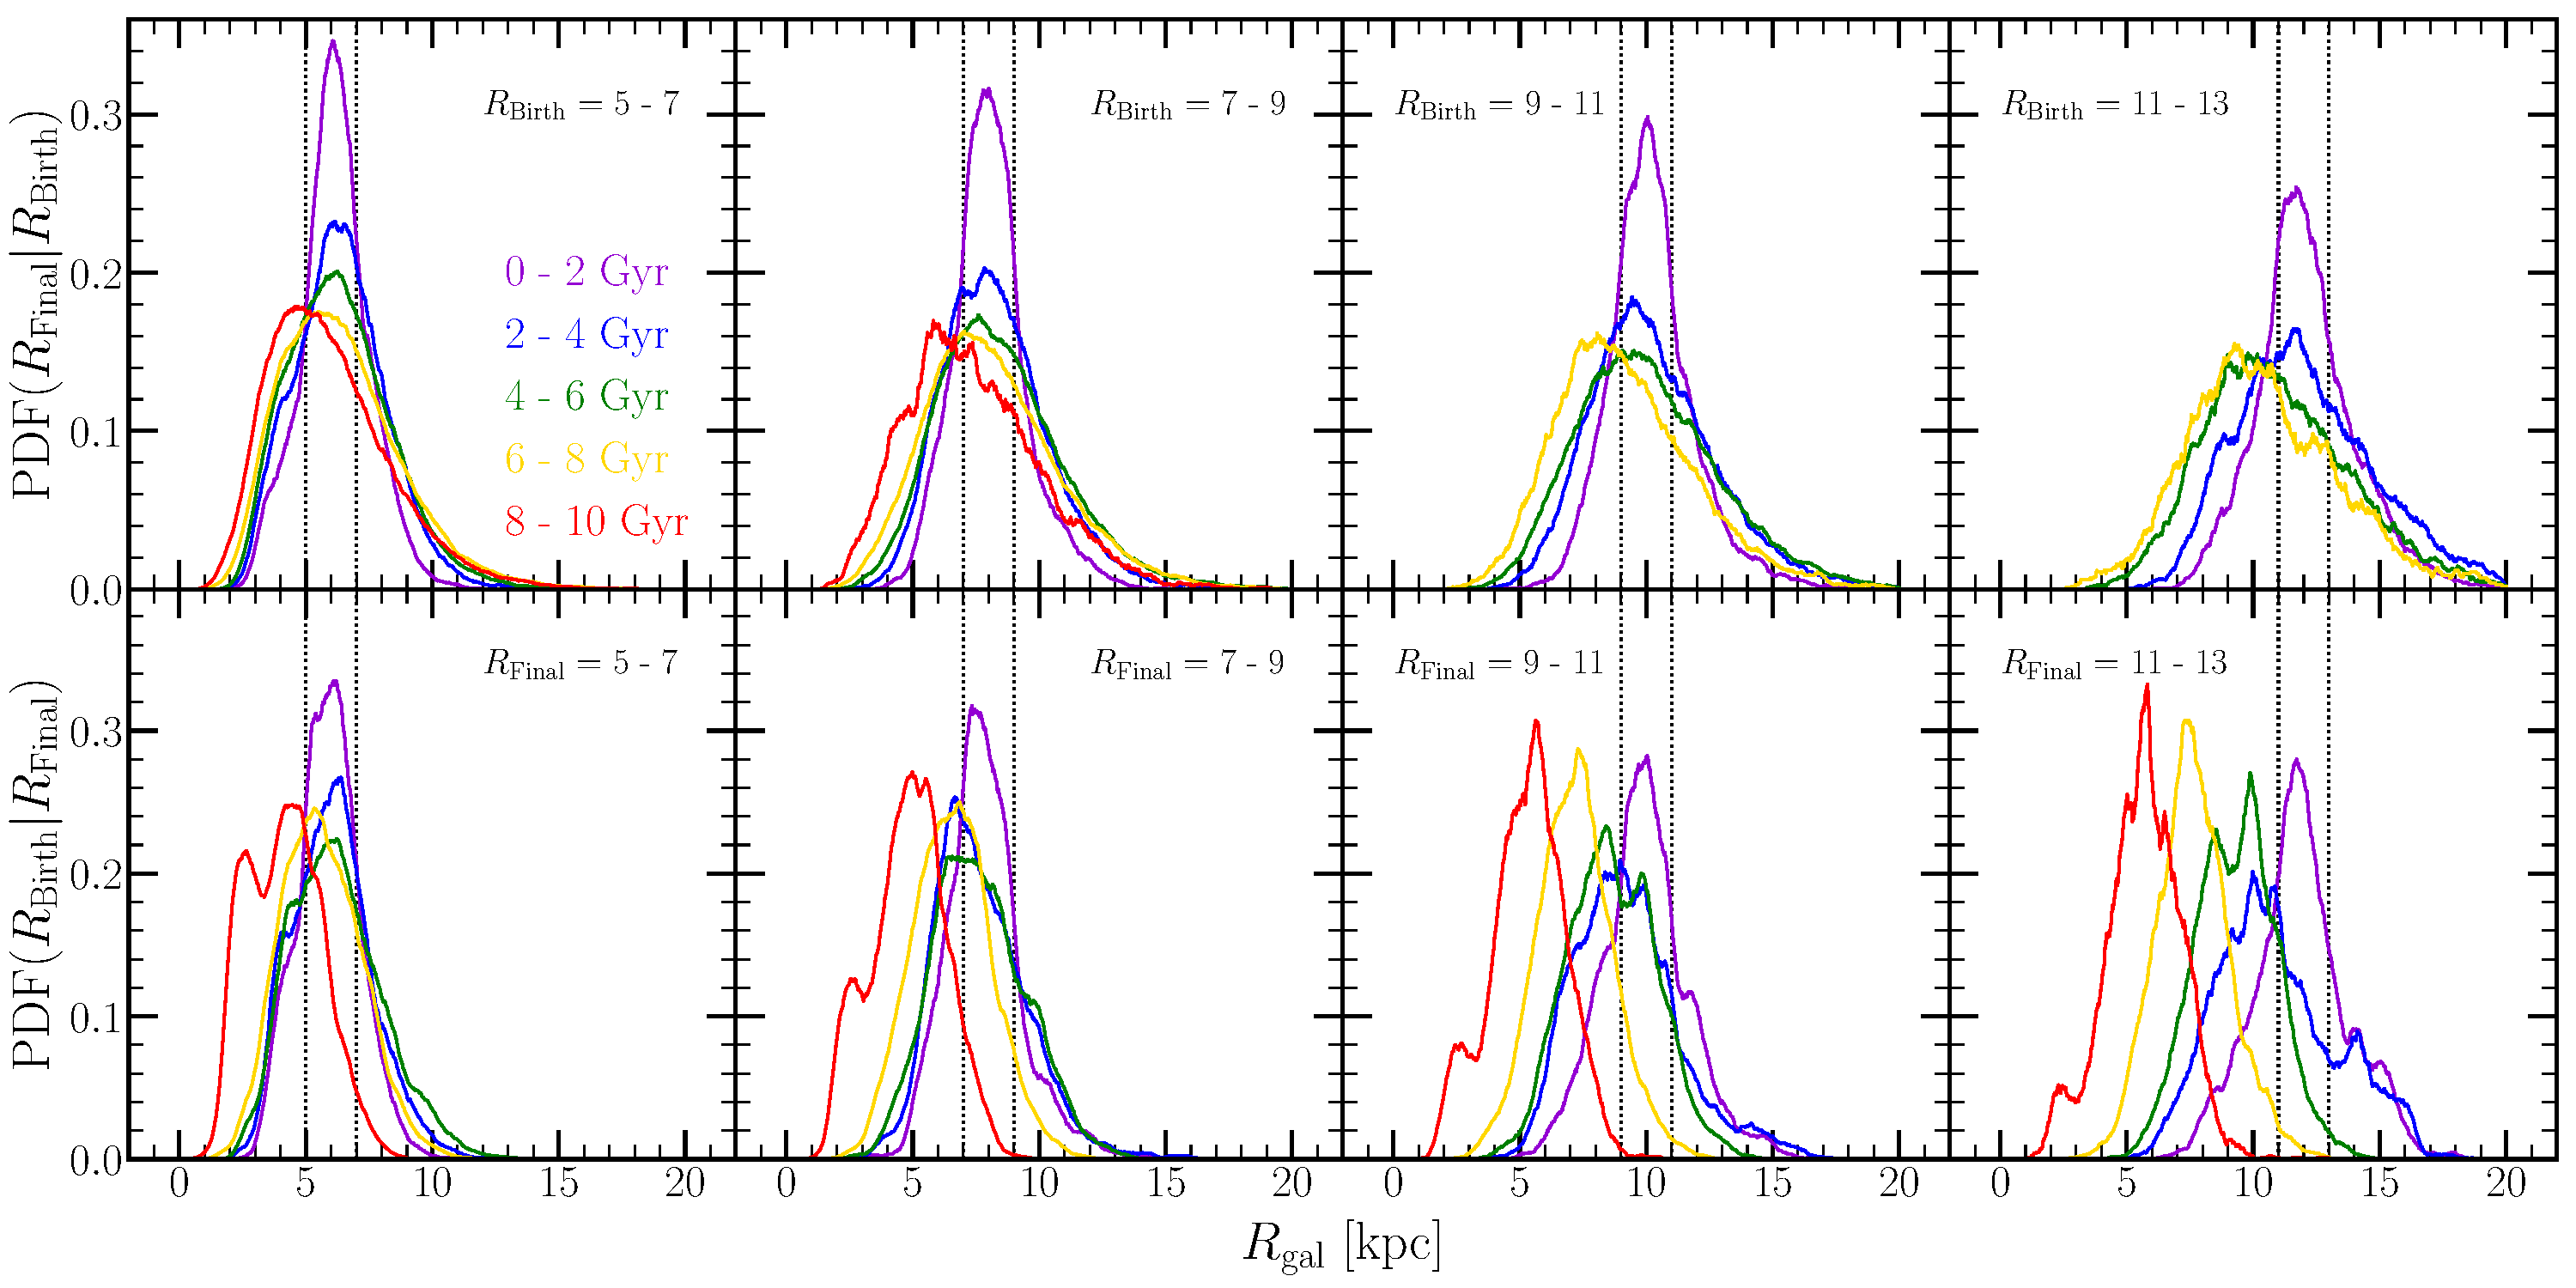
\includegraphics[scale = 0.32]{decomposition.pdf} 
\caption{Radial distributions of our candidate analog star particles 
from~\texttt{h277}. In the top row, we show distributions of~\textit{final} 
radius in bins of birth radius and age. In the bottom row, we show 
distributions of~\textit{birth} radius in bins of final radius and age. Each 
bin in Galactocentric radius is shown in its own panel, denoted in text at the 
top of each panel and by vertical black dashed lines. We color-code the 
distributions according to the age of the star particles, denoted by the 
legend in the upper left panel. We smooth all distributions with a box-car 
width of 0.5 kpc to improve clarity. We omit the distributions for 8 - 10 Gyr 
old stars born in the 9 - 11 and 11 - 13 kpc bins due to an insufficient 
number of star particles with which to calculate the distribution. }
\label{fig:h277_decomposition} 
\end{figure*} 

\begin{itemize} 
	\item In this paper we make use of star particles from the~\texttt{h277} 
	simulation~\citep{Christensen2012, Zolotov2012, Loebman2012, Loebman2014, 
	Brooks2014}. A synopsis of the detailed simulation parameters and 
	cosmological model can be found in~\S~2 of~\citet{Bird2020}. We do not 
	go into detail on that here, instead focusing on how we vet the sample of 
	star particles for use in our chemical evolution models. 

	\item We find that only~$\sim$3\% of~\texttt{h277}'s star particles formed 
	within the first 1 Gyr of its 13.7 Gyr run, indicating that $T$ = 1 Gyr 
	is a much better estimate of the onset of star formation and thus the 
	chemical evolution in~\texttt{h277} than $T$ = 0. We thus remove the star 
	particles that were born in the first Gyr of evolution, and subtract 1 Gyr 
	from their formation times, thus running our disc models for 12.7 Gyr. As 
	a result, our simulations run from a redshift of~$z \approx$ 3 to the 
	present day. 

	\item Of particular importance to have accurately measured formation radii 
	for each star particle that we use in our analysis.~\texttt{h277} did not 
	record the exact birth radius of each star particle; however, each star 
	particle does have an accurate age at each snapshot. If a star particle 
	is sufficiently young in the first snapshot it appears in, then its 
	radius in that snapshot is a reasonable approximation for its birth 
	radius, since its orbit is unlikely to have changed significantly in a 
	short enough time interval. Therefore, we restrict our sample to those 
	with an age at first snapshot of~$\leq$ 150 Myr, and adopt their 
	Galactocentric radius at first snapshot as the birth radius. Also 
	conducted the analysis with age at first snapshot of~$\leq$50 Myr, and 
	found similar results, suggesting this choice does not impact our 
	conclusions. In practice, we find that 150 Myr also provides us with an 
	adequately large number of star particles to sample from. 

	\item Based on a kinematic decomposition performed on the present-day 
	phase space distribution of the~\texttt{h277} star particles, we exclude 
	halo stars, but include bulge, pseudobulge, and thin- and thick-disc 
	stars. Even though we are not modeling the abundances in the bulge in this 
	paper, the bulge is believed to have formed in-situ ({\color{red} 
	citation}), while a significant fraction of halo stars are believed to 
	have been accreted ({\color{red} citation}). It's also likely that the 
	Milky Way bulge and disc exchanged statistically significant amounts of 
	stars and gas ({\color{red} citation}), coupling the chemical evolution of 
	the two at least slightly. This effect can be addressed in our models by 
	simply including these star particles in our sample. This yields a sample 
	of 3,019,521 star particles from~\texttt{h277}. 

	\item \texttt{h277} had a transient bar during its evolution, but does 
	not have a bar at $z$ = 0. This could mean that the star particles 
	in~\texttt{h277} migrated in a manner which does not reflect the dynamical 
	history of the Milky Way, but at present inferring a star's birth radius 
	observationally is notoriously difficult anyway ({\color{red} citation}), 
	so its likely the impact of this decision is within current 
	observational uncertainties. Nonetheless, it is worth noting that 
	the~\citet{Minchev2013} model, and by extension the~\citet{Minchev2014} 
	and~\citet{Minchev2017} studies as well, selected a hydrodynamical 
	simulation specifically so that it would have a bar at $z$ = 0. A detailed 
	investigation of the impact of bar evolution on stellar migration and thus 
	chemical evolution is outside the scope of this paper, though can be 
	conducted in principle by simply swapping the birth times and initial and 
	final radii of~\texttt{h277} within~\texttt{VICE}, rerunning the 
	simulations, and comparing the results. 

	\item Distributions of final radii in bins of birth radii and age are 
	shown in the top row of Fig.~\ref{fig:h277_decomposition}. Conversely, the 
	bottom row shows distributions of birth radii in bins of final radii and 
	age. 
	\begin{itemize} 
		\item Focusing on the top row of panels in 
		Fig.~\ref{fig:h277_decomposition}, we note that for stars born at any 
		radius and time, the distribution of final radii is still peaked near 
		the birth radius. With increasing age, it appears the mode final radius 
		may move slightly inward. The tails of the distributions to large radii 
		are relatively age-independent - some differences between the 0 - 2 and 
		8 - 10 Gyr age bins, but not much. However, the tails of the 
		distributions to small radii are not age-independent, and move toward 
		smaller $R_\text{gal}$ with increasing age. This suggests that radial 
		migration inward and outward occur on different timescales, in 
		particular that inward migration is slower than 
		outward migration. By extension this may suggest that inward and 
		outward migration are tied to different physical 
		processes.~\citet{Roskar2008a} demonstrate using a cosmological 
		simulation that resonant scattering at corotation causes stars to 
		move outward and gas to move inward. It's possible that radial 
		migration inward has different origins. 

		\item Focusing on the bottom row of panels in 
		Fig.~\ref{fig:h277_decomposition}, we note that the oldest stars at any 
		Galactocentric radius at the present day were overwhelmingly born at 
		smaller radii. The youngest stars, however, were overwhelmingly born at 
		comparable radii, and the stars of intermediate ages simply span the 
		range in radii between the two. With increasing radius, the 
		differences in the mode of the birth radius distribution between age 
		bins gets larger. 

		\item The differences in distributions shown in the top and bottom 
		panels boils down to stellar surface density being a strong function 
		of Galactocentric radius. Take for example the age = 8 - 10 Gyr bin in 
		both $R_\text{Birth}$ = 5 - 7 kpc and $R_\text{Final}$ = 11 - 13 kpc 
		bins (i.e. the red curves in the top-left and bottom-right panels). 
		For these old stars born at 5 - 7 kpc, 11 - 13 kpc is far down the tail 
		of the $R_\text{Final}$ distribution, and yet 5 - 7 kpc is the mode 
		$R_\text{Birth}$ of all old stars presently at these radii. This 
		implies that even though the majority of 8 - 10 Gyr old stars with 
		$R_\text{Final}$ = 11 - 13 kpc were born at 5 - 7 kpc, they make up 
		only a small fraction of the stars with similar birth radii. This is 
		only possible if the stellar surface density gradient is sufficiently 
		steep, which it is known to be~\citep[e.g.][]{Bland-Hawthorn2016}. 
		\begin{itemize} 
			\item Fig.~\ref{fig:h277_decomposition} also demonstrates that the 
			numbers of stars that migrated inward and outward are comparable 
			in~\texttt{h277}. Taking a~$\left|\Delta R_\text{gal}\right| \geq$ 
			500 pc between birth and final radii as the criterion for migrating 
			inward or outward, indeed we find that in our sample, 27\% 
			migrated inward, 29\% migrated outward, and the remaining 44\% 
			stayed near their birth radius. These are global percentages. 
		\end{itemize} 

		\item In all bins of birth radius, a good first-order estimate of the 
		probability density that a star has a final radius in the same bin 
		is~$\sim$0.3. With bins in radius on this plot of 2 kpc, this suggests 
		that ~$\sim$40\% of stars migrate significantly by the time 
		they're~$\sim$2 Gyr old. If the SN Ia DTD is a 
		$t^{-1.1} \approx t^{-1}$ power-law as suggested by recent 
		observations~\citep[e.g.][]{Maoz2012, Maoz2017}, 
		then we expect similar numbers of SN Ia events to occur with delay 
		times between 1 and 10 Gyr as we do between 100 Myr and 1 Gyr. With 
		such an extended DTD, and the distributions in final radius shown in 
		the bottom panel of Fig.~\ref{fig:h277_decomposition}, its possible 
		that white dwarfs migrate significant distances before producing a SN 
		Ia event. Indeed, in the ASAS-SN bright supernova catalog,~$\sim$10\% 
		of supernovae are seen at >10 kpc from their host galaxies 
		\citep{Holoien2019}. While this catalog is for~\textit{all} 
		supernovae, the majority of SN events are type Ia anyway. Based on 
		this, it's reasonable to expect that the migration 
		of nucleosynthetic yields may proceed alongside stellar migration, an 
		effect which is often neglected (e.g.~\citealp{Minchev2013}, and the 
		application of the~\citealp{Weinberg2017} analytic models in 
		\citealp{Feuillet2018}). In this paper, we relax this assumption. The 
		application of the~\texttt{h277} star particle data to our model for 
		radial migration and the time dependence thereof is discussed in the 
		next section. 

	\end{itemize} 

\end{itemize} 


\subsection{Radial Migration} 
\label{sec:methods:migration} 
\begin{itemize} 
	\item To simulate our models, we develop and make use of \texttt{VICE}'s 
	\texttt{milkyway} object, an extension of a more general object named 
	\texttt{multizone}. The \texttt{multizone} object is at its core an array 
	of \texttt{singlezone} objects, which are designed to handle 
	simulations of one-zone models and were the focus of 
	\citet{Johnson2020},~\texttt{VICE}'s initial release paper. The 
	\texttt{multizone} object then affords the user the ability to move 
	gas between zones with any given time dependence, and to assign all 
	stellar populations any given zone at any given time following their 
	birth, effectively allowing arbitrarily complex zone and migration 
	schema. The \texttt{milkyway} object is a user-friendly extension of this 
	which enforces a zone configuration in which the Galaxy is modeled as a 
	series of concentric annuli of uniform width~$\Delta R_\text{gal}$. As 
	defaults, it adopts the stellar migration model described in this section 
	{\color{red}and our star formation law described in~\S 
	\ref{sec:methods:sfe}.} 

	\item Stars in~\texttt{VICE} are stand-ins for entire stellar 
	populations, and in the~\texttt{milkyway} object, are said to be in a 
	given zone/annulus if their radius is between the inner and outer 
	edges. At all times, their nucleosynthetic products and returned envelopes 
	are placed in the ISM of the annulus that they are in~\textit{at that 
	time}. 

	\item Where hydrodynamical and N-body simulations of galaxy evolution 
	often use star particles of a fixed mass,~\texttt{VICE} forms a fixed 
	number of stellar populations in a given zone at a given timestep, 
	and allows their masses to vary to account for variations in the star 
	formation rate. The mass of stars formed in a given zone is divided 
	evenly among the stellar populations that form during a given 
	timestep. 

	\item Algorithm based on initial and final radii of star particles in 
	hydrodynamical simulations, for which we've taken~\texttt{h277} as 
	discussed in the previous section. 

	\item In modeling the Milky Way as a series of concentric annuli,
	~\texttt{VICE}'s~\texttt{milkyway} object assumes stellar populations to 
	be born at the centres of each annulus. 
	For a stellar population born at time $T$ and Galactocentric radius 
	$R_\text{gal}$, it searches for star particles from~\texttt{h277} that formed at $T \pm$ 300 Myr and $R_\text{gal} \pm$ 250 pc. It then randomly 
	selects a star particle from this subsample with no bias to act as 
	an~\textit{analog}. Adopts the final radius of the analog star particle at 
	face value, and moves from its radius of birth to the final radius at $T$ 
	= 12.7 Gyr with some time dependence. If no candidate analogs are found, 
	search is widened to $T \pm$ 600 Myr and $R_\text{gal} \pm$ 500 pc. If 
	still no candidate analogs are found in this widened search, the stellar 
	population is assumed to remain at its birth radius {\color{red} and to 
	have a final height above the disc midplane of $z$ = 100 kpc.} These 
	stellar populations are few in number. In our fiducial model with an 
	inside-out SFH (see~\S~\ref{sec:methods:sfhs}), these stellar populations 
	account for~$\sim$4.9\% of the simulated stellar populations by number, 
	but only~$\sim$0.56\% by mass. Making up such a small portion of the mass 
	budget, it's not likely they contribute significantly to the chemical 
	evolution of our model Galaxy. 
	\begin{itemize} 
		\item We have zones for each annulus from $R_\text{gal}$ = 0 to 
		20 kpc; there are no zones off the midplane. This retains the 
		assumption that the gas-phase abundances are vertically and 
		azimuthally well-mixed. Each stellar population simply assumes the 
		final height~$\left|z\right|$ above the disc midplane of its assigned 
		analog, though this doesn't enter into the simulations at all; it's 
		purely post-processing information. 
	\end{itemize} 

	\item When a star particle is assigned as an analog to a stellar 
	population in our simulations, it is~\textit{not} thrown out of the sample 
	of candidate analogs, in theory allowing a star particle to act as an 
	analog for multiple stellar populations. This is a difference between 
	the~\citet{Minchev2013} model and ours. Where we assign star particles to 
	stellar populations for which~\texttt{VICE} then calculates a stellar mass 
	and composition based on an assumed star formation history, the 
	\citet{Minchev2013} model assigns compositions to star particles. 

\begin{figure} 
\centering 
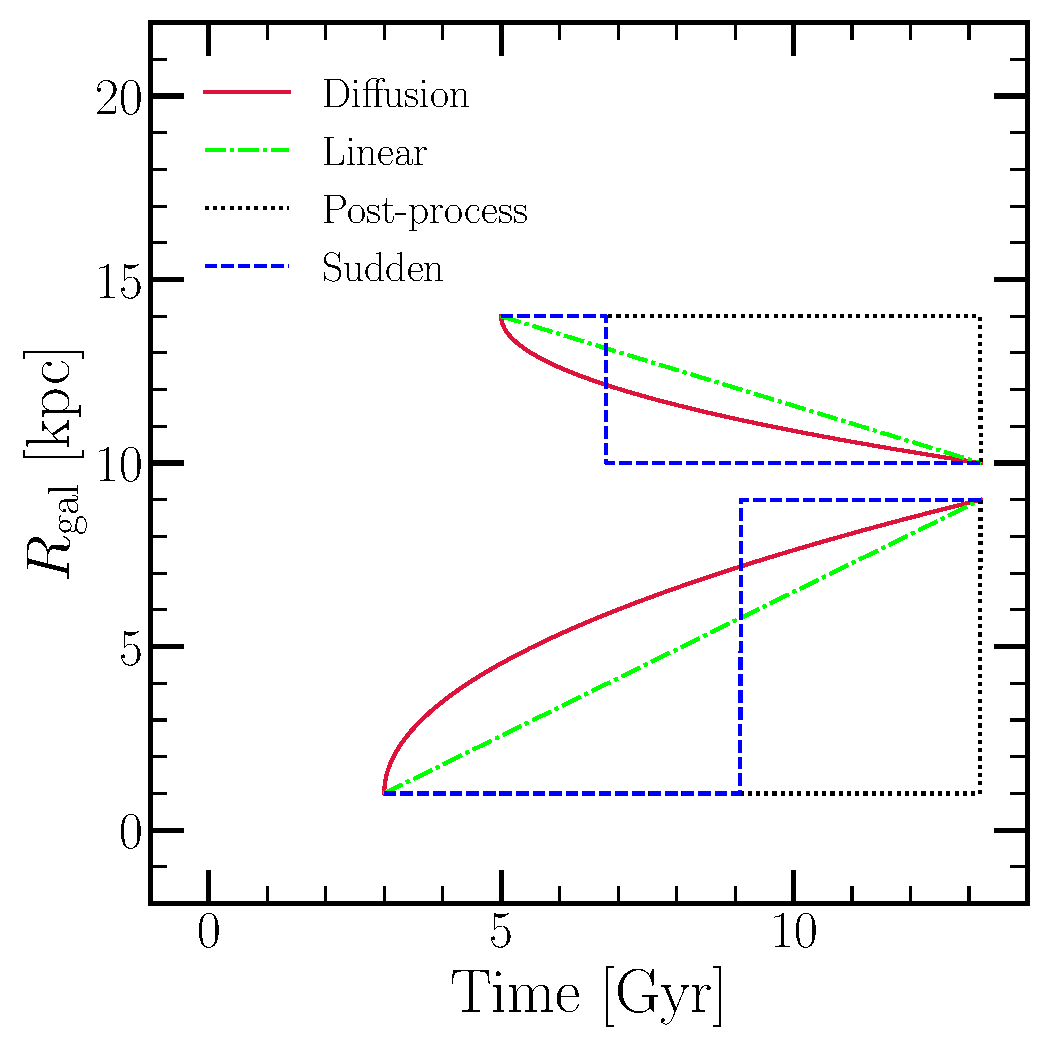
\includegraphics[scale = 0.45]{migration.pdf} 
\caption{A diagram illustrating how Galactocentric radius changes with time 
for two stellar populations under our migration schema: diffusion (crimson, 
solid), linear (lime, dot-dashed), post-process (black, dotted), and 
sudden (blue, dashed). Here the initial and final radii and birth times are 
chosen at random for illustrative purposes. With the initial and final 
Galactocentric radii of a stellar population, its birth time, and one of these 
assumptions about the time-dependence of migration, the Galactocentric radius 
at all times is known. } 
\label{fig:migration_schema} 
\end{figure} 

	\item Our migration models 
	\begin{itemize} 
		\item All neglect radial gas flows, this paper instead focusing on 
		four simple models for how the radius of a stellar population's orbit 
		changes with time. Investigation of our models with radial gas flows 
		would be an interesting extension to this paper. 

		\item \textbf{Post-processing}: Stars stay where they are born until 
		the final timestep. Based on the assumption that stellar populations 
		do not contribute to enrichment beyond their birth 
		radius~\citep[e.g.][]{Minchev2013}. Each annulus simulated as a 
		one-zone model independent of all other zones. Shown in black dotted 
		line in Fig.~\ref{fig:migration_schema}. 

		\item \textbf{Sudden}: A random number is drawn from a uniform 
		distribution between the time of birth and the present day. That time 
		is taken to be the time of instantaneous migration to the present-day 
		annulus. Emulates a scenario in which a single dynamical interaction 
		changes the orbital radius of a star. Can be thought of as a 
		time-dependent extension of the post-processing scenario. Shown in 
		blue dashed line in Fig.~\ref{fig:migration_schema}. 

		\item \textbf{Diffusion}: A case in which stars migrate in a 
		continuous, time-dependent manner. If stars move to their final 
		radii via a random walk, then the mean displacement of stars that 
		migrate similar distances would scale with~$\sqrt{\text{age}}$. This 
		is shown in the red solid line in Fig.~\ref{fig:migration_schema}. 
		This is our fiducial migration model; we present results using this 
		model except where otherwise noted. It is so named because it 
		corresponds to a scenario in which the random walk carries out the 
		diffusion of angular momentum. 

		\item \textbf{Linear}: A simple variation of the 
		diffusion model. Has no physical motivation other than numerical 
		ease, but together with the diffusion model constitutes a test of how 
		sensitive our models are to the assumed time-dependence of stellar 
		migration. Demonstrated by green dot-dashed line in 
		Fig.~\ref{fig:migration_schema}. 
	\end{itemize} 

	\item Further details on the implementation of the~\texttt{milkyway} 
	object, the more general~\texttt{multizone} object, and other features of 
	\texttt{VICE} can found in its documentation.~\footnote{
		\url{https://vice-astro.readthedocs.io} 
	}

	\item We have a sample of 3,019,521 candidate analog star particles 
	from~\texttt{h277}, only~$\sim$57\% of which are disc stars. Since we're 
	modeling the thin and thick disc populations here,~$\sim$1.72 million is a 
	much better estimate of the number of analogs that we can realistically 
	sample from. We let star formation extend out to 15.5 kpc, beyond which 
	we force the star formation rate to zero at all times.~\texttt{VICE} does 
	form stellar populations at all timesteps in the annuli; they simply have 
	zero mass and thus do not contribute to the chemical evolution or 
	recycling, though they do contribute to the computational overhead. We 
	take $\Delta R_\text{gal}$ = 100 pc as the width of each annulus from 
	$R_\text{gal}$ = 0 to 20 kpc and a timestep size of $\Delta T$ = 10 Myr 
	from $T$ = 0 to 12.7 Gyr (see discussion in~\S~\ref{sec:methods:h277} for 
	our choice of time-interval). With the resulting 200 zones and 1,271 
	timesteps, we let~\texttt{VICE} form~$n$ = 8 stellar 
	populations per zone per timestep, resulting in 2,033,600 stellar 
	populations with predicted masses and abundances, 1,574,800 of which form 
	between~$R_\text{gal}$ = 0 and 15.5 kpc and have nonzero mass, reasonably 
	within the limit of what we can sample. These simulations run in~$\sim$2 
	hours and take up~$\sim$235 MB of disc space per output, including the 
	extra data that we record for each stellar population's analog star 
	particle. 
\end{itemize} 


\subsection{Nucleosynthetic Yields, Outflows, and Recycling}  
\label{sec:methods:yields} 
\begin{itemize} 
	% \item Brief background on~\texttt{VICE}'s algorithm: we form a given 
	% number of stellar populations in each zone and at each timestep. They 
	% then migrate between zones according to our algorithm and eject CCSN and 
	% SN Ia products as smooth functions of time according to our yields. 

	\item \textit{Fractional net} yields, as required by~\texttt{VICE}. 
	Recycling is implemented separately, such that stellar envelopes are 
	returned to the ISM at the birth composition of each stellar population. 
	\texttt{VICE} takes the general approach of returning previously produced 
	material according to a stellar lifetime model and injecting newly 
	produced nucleosynthetic products as described below. Also clarify that 
	these are not~\textit{effective} yields in that outflows are also 
	implemented separately. 

	\item CCSN events are assumed to occur immediately following the formation 
	of their progenitor stars. This is an adequate approximation, because the 
	lifetimes of massive stars are short compared to the relevant timescales 
	for galaxy evolution. For the most massive stars, the lifetimes are 
	comparable to the timestep size that we take use in these simulations 
	anyway. This assumption implies a linear relationship between CCSN 
	enrichment and the star formation rate: 
	\begin{equation} 
	\dot{M}_x^\text{CC} = y_x^\text{CC}\dot{M}_\star 
	\end{equation} 
	\begin{itemize} 
		\item Physically, the CCSN yield $y_x^\text{CC}$ is the fraction of a 
		stellar population's initial mass that is converted into some element 
		$x$ and ejected to the ISM, neglecting outflows. 

		\item \texttt{VICE} includes functionality with which to calculate 
		the value of $y_x^\text{CC}$ for a handful of nucleosynthetic yield 
		studies. Details can be found in~\S~2 of~\citet{Johnson2020} and in 
		\texttt{VICE}'s documentation. A detailed investigation of 
		CCSN nucleosynthetic yields which releases new features to these 
		calculations will be presented in Griffith et al. (2021, in prep). 

		\item Take $y_\text{O}^\text{CC}$ = 0.015 and $y_\text{Fe}^\text{CC}$ 
		= 0.0012 from~\citet{Johnson2020}, who in turn adopt these values 
		from~\citet{Weinberg2017}. 
	\end{itemize} 

	\item SN Ia products injected with a $t^{-1.1}$ delay-time distribution 
	(DTD) with a minimum delay-time of $t_\text{D}$ = 150 Myr. This is the 
	default DTD in~\texttt{VICE}, adopted in~\citet{Johnson2020}, and is 
	suggested by recent observational results comparing the cosmic SN Ia rate 
	to the cosmic SFH~\citep{Maoz2012, Maoz2017}. In a 
	one-zone model at times $t > t_\text{D}$, the enrichment rate for some 
	element~$x$ can be expressed as the product of some yield $y_x^\text{Ia}$ 
	and the star formation history weighted by the DTD: 
	\begin{subequations}\begin{align} 
	\dot{M}_x^\text{Fe} &= y_x^\text{Fe}\langle\dot{M}_\star\rangle_\text{Ia} 
	\label{eq:mdot_ia} 
	\\ 
	&= y_x^\text{Fe} \ddfrac{
		\int_0^{t - t_\text{D}} \dot{M}_\star(t') R_\text{Ia}(t - t') dt' 
	}{
		\int_{t_\text{D}}^{t_\text{max}} R_\text{Ia}(t - t') dt' 
	} 
	\label{eq:mdot_ia_expanded} 
	\end{align}\end{subequations} 
	where $R_\text{Ia}$ is the DTD itself, in units of M$_\odot^{-1}$ 
	Gyr$^{-1}$. Like the CCSN yield,~$y_x^\text{Ia}$ is simply the fraction of 
	a single stellar population's mass that is converted into the element~$x$ 
	over the ensuing SN Ia duty cycle. It can also be expressed as an integral 
	over the DTD: 
	\begin{equation} 
	y_x^\text{Ia} = m_x^\text{Ia} \int_{t_\text{D}}^{t_\text{max}} 
		R_\text{Ia}(t) dt = m_x^\text{Ia} \frac{N_\text{Ia}}{M_\star} 
	\label{eq:y_x_ia} 
	\end{equation} 
	where the~$m_x^\text{Ia}$ is the mass of some element~$x$ produced in a 
	single SN Ia event on average, and the integral evaluates to the mean 
	number of Ia events~$N_\text{Ia}$ per mass of stars formed~$M_\star$. 
	\begin{itemize} 
		\item \texttt{VICE} enforces~$t_\text{max}$ = 15 Gyr always, though 
		provided one is consistent with equations~\refp{eq:y_x_ia} and 
		\refp{eq:mdot_ia_expanded}, the results are independent of 
		$t_\text{max}$ since the integrals cancel. 

		\item Extending this to multi-zone models is simple - rather than an 
		integral over the star formation history of a given annulus, the rate 
		becomes a summation over all stellar populations that are in a given 
		zone at some time: 
		\begin{equation} 
			\dot{M}_x^\text{Ia} = y_x^\text{Ia} \ddfrac{
				\sum_i M_i R_\text{Ia}(\tau_i) 
			}{
				\int_{t_\text{D}}^{t_\text{max}} R_\text{Ia}(t) dt 
			} 
		\end{equation} 
		where~$M_i$ and~$\tau_i$ are the mass and age of the~$i$'th stellar 
		population, respectively. 

		\item Initially adopt~$y_\text{O}^\text{Ia}$ = 0 and 
		$y_\text{Fe}^\text{Ia}$ = 0.0017 from~\citet{Johnson2020} and 
		\citet{Weinberg2017}. However, in practice we find that the e-folding 
		timescales of star formation in our models are sufficiently long (see 
		discussion in~\S~\ref{sec:methods:sfhs}) such that our fiducial, 
		inside-out SFH model predicts [O/Fe]~$\approx$~+0.05 for 
		young stars. We therefore multiply this value by a factor of 
		10$^{0.1}$, adopting instead~$y_\text{Fe}^\text{Ia}$ = 0.00214 so 
		that our fiducial model predicts a late-time [O/Fe] ratio in better 
		agreement with observations. This change is likely within the 
		uncertainties in nucleosynthetic yields anyway. 

		\item Our model assumes that all supernova yields of O and Fe are 
		independent of metallicity. While this appears to be empirically true 
		for CCSN yields of these elements~\citep[e.g.][]{Weinberg2019, 
		Griffith2020}, recent evidence by~\citet{Brown2019} suggests that 
		the local specific SN Ia rate shows a strong, inverse dependence on 
		galaxy stellar mass. They argue that this may imply a metallicity 
		dependent~$R_\text{Ia}$ that produces more SN Ia events at early times 
		when the metallicity is low. While we adopt a metallicity independent 
		$y_\text{Fe}^\text{Ia}$ in this paper,~\texttt{VICE} allows users to 
		specify any functional form for $y_\text{Fe}^\text{Ia}$ as a function 
		of the total abundance by mass $Z$, allowing future studies of the 
		impact of this to proceed straight-forwardly. 
	\end{itemize} 

	\item Similar to SN Ia, the equation detailing asymptotic giant brach 
	(AGB) star enrichment changes from an integral over the SFH to a summation 
	over the stellar populations in a given zone at some time.~\texttt{VICE} 
	in its current iteration forces AGB enrichment to be included in its 
	simulations, though the yields of O and Fe from AGB stars are negligible 
	compared to their supernova yields, and the results presented in this 
	paper can be interpreted as if they were zero. 
	\begin{itemize} 
		\item The algorithm is based on determining the fraction of a single 
		stellar population's mass that is in the form of stars that will have 
		ended their post-main-sequence lifetime during the next timestep. 
		The mass of those stars and their birth metallicity can then be 
		used to determine a yield given a table of $y_x^\text{AGB}$ values 
		sampled on a grid of stellar mass and metallicity, for which we take 
		values from the FRUITY database of net yeilds~\citep{Cristallo2011}. 
		Since these yields are not important for this paper, however, we do 
		not go into further detail. More information on \texttt{VICE}'s 
		treatment of AGB enrichment can be found in its documentation and in 
		\S~2.6 of~\citet{Johnson2020}. 
	\end{itemize} 

	\item Outflows are directly tied to nucleosynthetic yields, because the 
	absolute scaling of nucleosynthetic yields and the efficiency with which 
	galactic winds remove them from the star forming reservoir determine the 
	\textit{effective} yield: the amount of metals that are not only produced 
	but added to the star forming reservoir. 
	\begin{itemize} 
		\item Based on studies of galactic fountains demonstrating that 
		ejected metals tend to fall back to a similar radius at which they 
		were produced~\citep[e.g.][]{Melioli2008, Melioli2009, Spitoni2008, 
		Spitoni2009}, a number of chemical evolution models 
		\citep[e.g.][]{Minchev2013, Spitoni2019} neglect outflows, arguing 
		that they are not a necessary ingredient to chemical evolution models. 
		However, with the yields we've adopted, our models require significant 
		metal ejection to predict realistic abundances. For this reason, 
		studies which neglect outflows adopt significantly lower 
		nucleosynthetic yields as a consequence. 

		\item There is a near one-to-one degeneracy between the scaling of 
		nucleosynthetic yields and the efficiency of metal ejection in 
		galaxies. With nucleosynthetic yields that were conventional at the 
		time,~\citet{Dalcanton2007} demonstrated that significant outflows 
		are required to lower effective yields and predict abundances in 
		agreement with observations. This is a solution to the so-called 
		``G-dwarf problem'' in which closed-box models of chemical evolution 
		\citep[see the review in, e.g.,][]{Tinsley1980}  catastrophically 
		over-predict the number of super-solar metallicity stars 
		\citep{vandenBergh1962, Pagel1975}. However, recent findings with 
		regard to black hole formation and stellar explodability have 
		demonstrated that many massive stars simply do not produce a supernova 
		event (see theoretical discussion by, e.g.,~\citealp{Pejcha2015, 
		Sukhbold2016}, and observation evidence from~\citealp{Gerke2015, 
		Adams2017, Basinger2020}). This challenges the results of 
		\citet{Dalcanton2007}, suggesting that nucleosynthetic yields are 
		intrinsically low, and the extent to which theoretically predicted 
		stellar explodability models reduce the need for outflowing winds 
		remains an unanswered question for future studies. 
	\end{itemize} 

	\item Mass-loading factor $\eta$ defined as the ratio of mass outflow 
	rates from the ISM to the SFR: 
	\begin{equation} 
	\eta \equiv \frac{\dot{M}_\text{out}}{\dot{M}_\star} 
	\end{equation} 
	\citet{Weinberg2017} demonstrate that, to first order, this parameter and 
	the yields of a given element set the late-time equilibrium abundance. 
	Here we adopt a scaling of~$\eta$ with Galactocentric radius~$R_\text{gal}$ 
	such that the equilibrium abundance as a function of~$R_\text{gal}$ 
	reproduces a metallicity gradient in agreement with observations. 

	\item A fundamental observable, the observed metallicity gradient in the 
	Milky Way has been the focus of a considerable number of studies to date. 
	\begin{itemize} 
		\item \citet{Nordstroem2004a} find a gradient of -0.099 kpc$^{-1}$ in 
		[Fe/H] in main sequence stars from GCS~\citep{Nordstroem2004b, 
		Holmberg2007}. 

		\item \citet{Daflon2009} find a gradient of -0.04 kpc$^{-1}$ in 
		[S/H] in OB stars 

		\item \citet{Frinchaboy2013} find a gradient of -0.09 kpc$^{-1}$ in 
		[M/H] in open clusters. 

		\item \citet{Hayden2014} also find -0.09 kpc$^{-1}$ in [M/H] for 
		$R_\text{gal}\gtrsim$ 6 kpc for low-$\alpha$ stars. For 
		$R_\text{gal}\lesssim$ 6 kpc, they find a relatively flat gradient. 

		\item \citet{Weinberg2019} finds -0.06 kpc$^{-1}$ in mode([Mg/H]) for 
		upper red giant branch disc stars (see their Fig. 23). 
	\end{itemize} 

	\item The procedure outlined in this section makes two assumptions: 1) 
	that the mode abundance at a given radius reflects the equilibrium 
	value at that radius, and 2) that radial migration does not significantly 
	impact the overall form of the gradient. We demonstrate that this holds in 
	our simulations in~\S~\ref{sec:metallicity_gradient}. 

	\item For $\alpha$ elements,~\citet{Weinberg2017} defines the equilibrium 
	abundance under a constant SFH as: 
	\begin{equation} 
	Z_{\alpha,\text{eq}} = \frac{
		y_\alpha^\text{CC}
	}{
		1 + \eta(R_\text{gal}) - r
	} 
	\end{equation} 
	where $r$ is the recycling parameter ($\approx$ 0.4 for the sake of this 
	scaling with a~\citetalias{Kroupa2001} IMF; see discussion near the end of 
	this section). Solving for $\eta(R_\text{gal})$ yields: 
	\begin{equation} 
	\eta(R_\text{gal}) = \frac{
		y_\alpha^\text{CC}
	}{
		Z_{\alpha,\text{eq}}
	} + r - 1 
	= \frac{y_\alpha^\text{CC}}{Z_{\alpha,\odot}}10^{-\text{mode([X/H])}
	(R_\text{gal})} + r - 1 
	\end{equation} 

	\item We assume a slope of -0.08 kpc$^{-1}$, in tentative agreement with 
	the previous studies that quote the slope of the gradient mentioned above. 
	To set the normalization, we assume the mode([X/H]) to be~$\sim$+0.3 at 
	$R_\text{gal}$ = 4 kpc, since this would produce mode([X/H])~$\approx$~0 at 
	$R_\text{gal}\approx$ 7 - 9 kpc. This results in the following form for 
	$\eta$ as a function of Galactocentric radius: 
	\begin{equation} 
	\eta(R_\text{gal}) = \frac{y_\alpha^\text{CC}}{Z_{\alpha,\odot}} 
	10^{(-0.08\text{ kpc}^{-1})(R_\text{gal} - \text{4 kpc}) + 0.3} + r - 1 
	\label{eq:eta} 
	\end{equation} 
	where we adopt our yield of O for $y_\alpha^\text{CC}$ and the solar 
	abundance of O of $Z_{\text{O},\odot}$ = 0.00572 from~\citet{Asplund2009}. 

	\item This does assume a uniformly linear gradient at all $R_\text{gal}$. 
	\citet{Hayden2014} do find the gradient in [M/H] to flatten for 
	$R_\text{gal}\lesssim$ 6 kpc, challenging this assumption. However, this 
	procedure can be easily repeated for any desired gradient, since the 
	functional form simply goes into the power of 10 in equation~\refp{eq:eta}. 

	\item The top panel of Fig.~\ref{fig:eta_tau_sfh} plots this scaling of 
	$\eta$ with~$R_\text{gal}$, highlighting a value of~$\sim$2.15 for the 
	solar circle in the red dotted line. 
\end{itemize} 

\begin{figure} 
\centering 
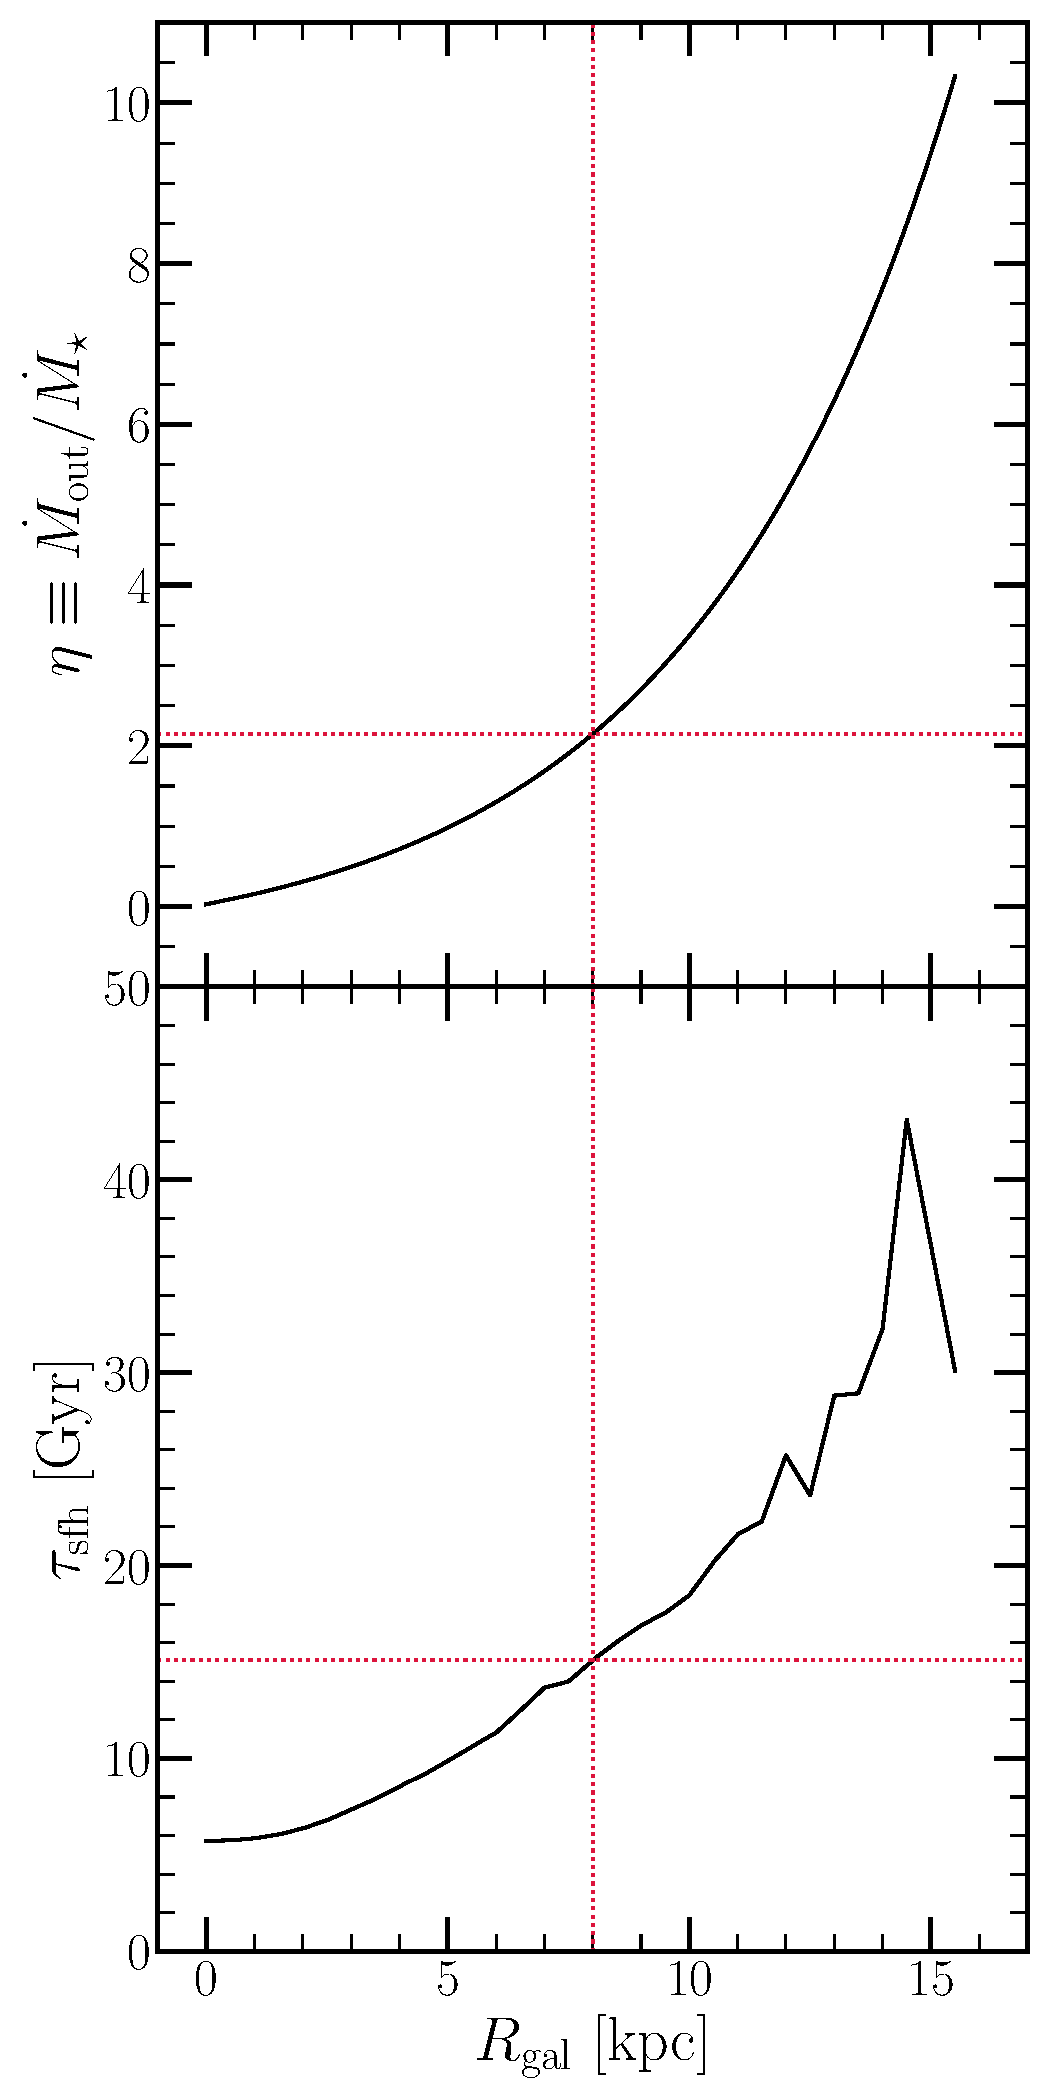
\includegraphics[scale = 0.65]{eta_tau_sfh.pdf} 
\caption{\textbf{Top}: Our implemented scaling of the mass loading factor 
$\eta$~with Galactocentric radius (black) as defined by equation 
\refp{eq:eta}.~\textbf{Bottom}: The e-folding timescales of the star formation 
histories of our model galaxies (black). These values come from a fit to the 
$\Sigma_\star$-age relation in bins of $R/R_\text{e}$ for~$10^{10.5}$~- 
$10^{11}$~M$_\odot$~Sa/Sb Hubble type spiral galaxies as reported by 
\citet[][see discussion in~\S~\ref{sec:methods:sfhs}]{Sanchez2020}. The 
horizontal and vertical red dashed lines in both panels highlight a mass 
loading factor of~$\eta \approx$ 2.15 and a star formation timescale of 
$\tau_\text{sfh} \approx$ 15 Gyr at an assumed radius of the sun of 
$R_\odot$ = 8 kpc. 
} 
\label{fig:eta_tau_sfh} 
\end{figure} 

\begin{itemize} 
	\item \citet{Weinberg2017} defined the~\textit{cumulative return fraction}
	$r$ to be the fraction of a single stellar population's initial mass that 
	has been returned to the ISM. In detail, $r$ is a complicated function of 
	the age of a stellar population $\tau$ which depends on the assumptions 
	about stellar lifetimes, the IMF, and an initial-remnant mass 
	relation~\citep[e.g.][]{Kalirai2008}. 
	\begin{itemize} 
		\item \citet{Weinberg2017} demonstrated that the assumption 
		of~\textit{instantaneous recycling} is a reasonable approximation, 
		where instantaneous recycling refers only to~\textit{previously 
		produced} nucleosynthetic products. We clarify that previous studies 
		have made this approximation for newly produced material as well; 
		while that assumption is valid for prompt sources like CCSNe, it fails 
		for enrichment channels with significant DTDs, such as SNe Ia or 
		AGB stars.~\citet{Weinberg2017} demonstrate that $r$ = 0.4 (0.2) is a 
		good approximation for a~\citetalias{Kroupa2001} (
		\citetalias{Salpeter1955}) IMF. However, this was demonstrated for 
		smooth star formation histories 
		and in parameter spaces conducive to analytic solution. Because 
		numerical integration of $r(\tau)$ is neither challenging nor 
		time-consuming,~\texttt{VICE} by default implements continuous 
		recycling by solving $r(\tau)$ at the beginning of each simulation 
		given the IMF, the~\citet{Kalirai2008} initial-remnant mass model, and 
		the assumption that $\tau = \tau_\odot(M/M_\odot)^{-3.5}$. We also 
		assume a post-main sequence lifetime of 10\% of the main sequence 
		lifetime for all stars. Further details on the detailed form of 
		$r(\tau)$ and its numerical integration within~\texttt{VICE} can be 
		found in its documentation. 
	\end{itemize} 

	\item In a one-zone model, the recycling rate can be expressed as an 
	integral over the star formation history: 
	\begin{equation} 
	\dot{M}_x^\text{r} = \int_0^t Z_x(t') \dot{M}_\star(t') \dot{r}(t - t') dt' 
	\end{equation} 
	where $Z_x$ is the abundance by mass of the element~$x$ in the ISM at a 
	time $t'$. Like SN Ia enrichment rates, extending this to multi-zone models 
	changes the integral over the star formation history to a summation over 
	the stellar populations in a given zone at some time: 
	\begin{equation} 
	\dot{M}_x^\text{r} = \sum_i Z_{x,i} M_i \dot{r}(\tau_i) 
	\end{equation} 
	In the case of the gas recycling rate, the equation has the same form, but 
	without the weighting by metallicity. 

	\item We implement continuous recycling in our simulations, but make use 
	of the instantaneous approximation in a handful of places in this paper 
	(e.g. in our scaling of $\eta$ with $R_\text{gal}$, and in approximating 
	SN Ia rates in~\S~\ref{sec:metallicity_space}). 
\end{itemize} 

\subsection{Star Formation Histories} 
\label{sec:methods:sfhs} 

\begin{figure*} 
\centering 
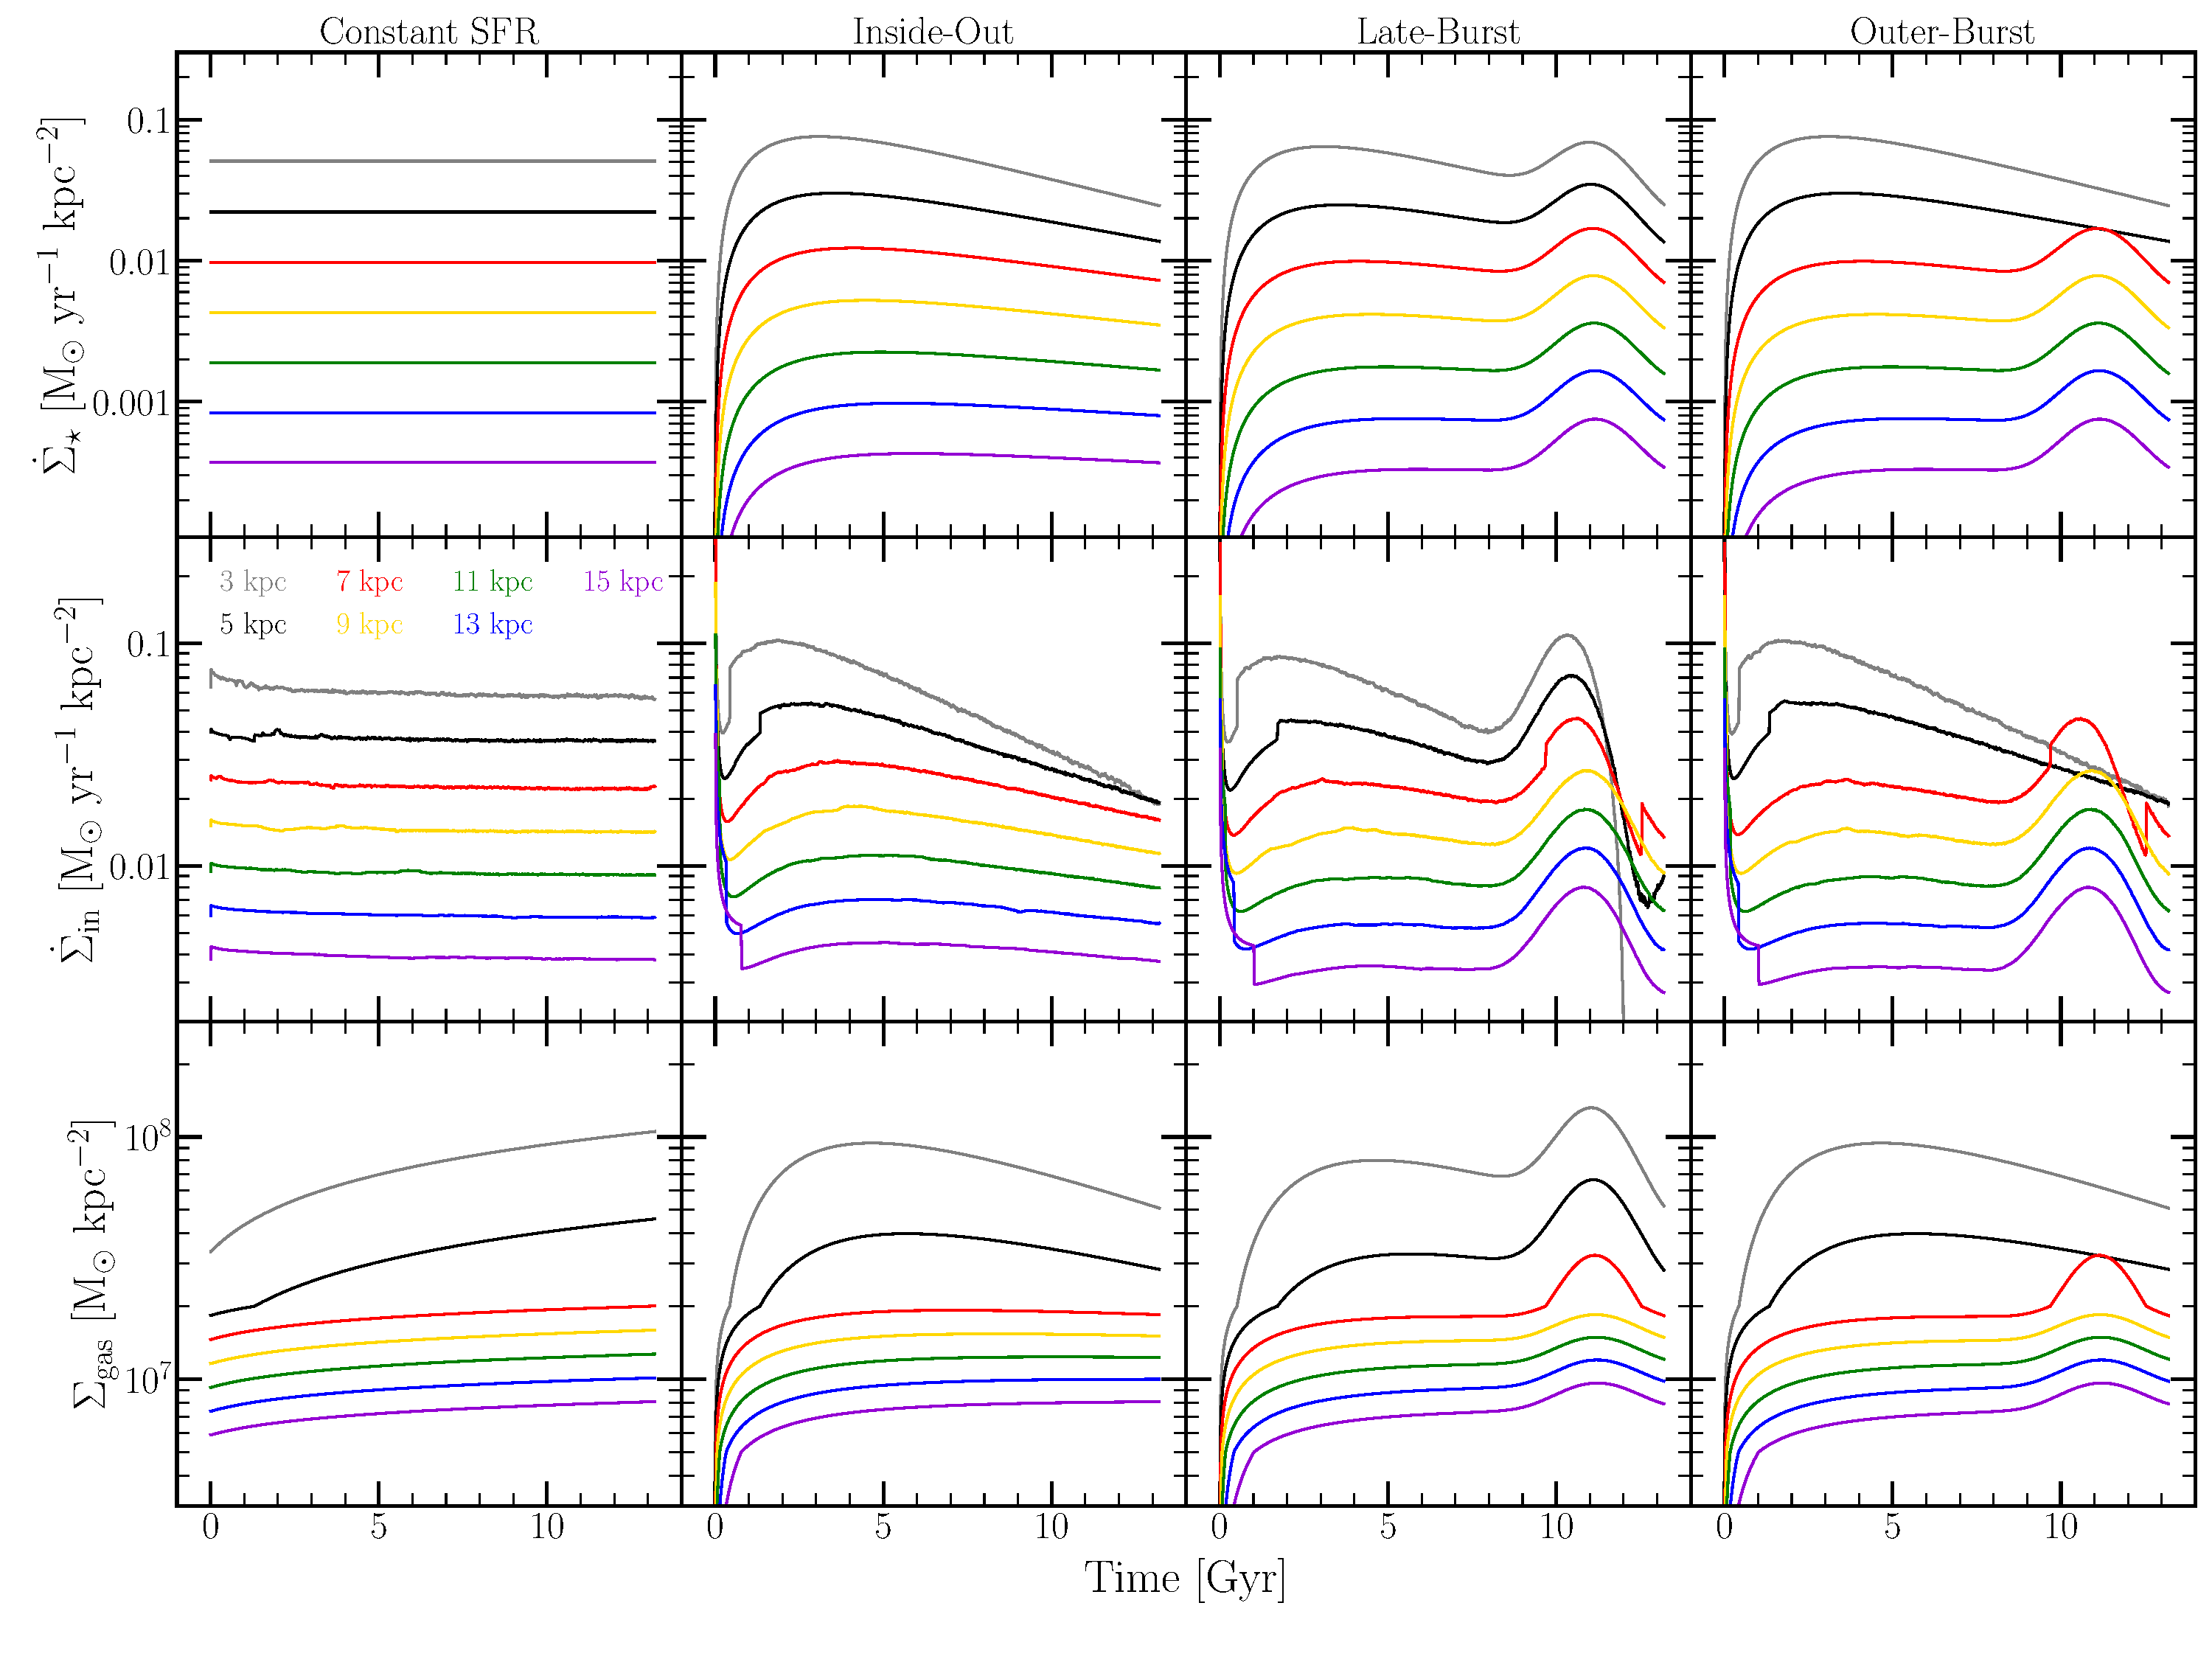
\includegraphics[scale = 0.32]{evol.pdf} 
\caption{The surface densities of star formation $\dot{\Sigma}_\star$ (top 
row), infall $\dot{\Sigma}_\text{in}$ (middle row), and gas $\Sigma_\text{gas}$ 
(bottom row) as functions of simulation time for our four fiducial SFHs: 
constant (far left), inside-out (left middle), late-burst (right-middle), 
and outer-burst (far right). We plot curves for the annuli whose inner radii 
are 3 kpc (grey), 5 kpc (black), 7 kpc (red), 9 kpc (yellow), 11 kpc (green), 
13 kpc (blue), and 15 kpc (purple) (see equations~\refp{eq:constant_sfh}, 
\refp{eq:insideout_sfh},~\refp{eq:lateburst_sfh}, and~\refp{eq:outerburst_sfh} 
for the mathematical definition of each SFH). } 
\label{fig:evol} 
\end{figure*} 

\begin{itemize} 
	\item \texttt{VICE}'s simulations runs in either infall, star formation, or 
	gas mode, referring simply to which component of the evolutionary history 
	the user has specified. The fiducial starburst models presented in 
	\citet{Johnson2020} ran in infall mode, but here we run things in star 
	formation mode, since we are after specific forms for the star formation 
	histories of our models. 

	\item Appendix~\ref{sec:normalize_sfh} presents justification of how we 
	normalize the parameters of our star formation histories to produce a 
	realistic model Galaxy at the end of the simulation. In short, it takes in 
	a unitless description of the time-dependence of the SFH at a given 
	Galactocentric radius, denoted $f(t|R_\text{gal})$, and a unitless 
	description of the radial dependence of the present-day stellar surface 
	density, denoted $g(R_\text{gal})$. In short, we integrate 
	$f(t|R_\text{gal})$ with time for each annulus, assuming $R_\text{gal}$ to 
	correspond to the centre of the zone, and attach a prefactor to 
	$f(t|R_\text{gal})$ at each $R_\text{gal}$ such that the desired gradient 
	is achieved with a total stellar mass similar to that of the Milky Way. 
	This procedure neglects the impact of radial migration, assuming that it 
	does not significantly alter the form of $g(R_\text{gal})$. We demonstrate 
	that these assumptions hold in~\S 
	\ref{sec:methods:surface_density_gradient}, in which we also detail our 
	adopted form of $g(R_\text{gal})$. As long as this assumption is not 
	violated, the equation derived in Appendix~\ref{sec:normalize_sfh} can be 
	used to normalize the parameters of future models of spiral galaxies. 

	\item We present four fiducial SFHs, which we dub ``constant'', 
	``inside-out'', ``late-burst'', and ``outer-burst''. They're defined as 
	follows: 
	\begin{itemize} 
		\item \textbf{Constant}: The SFH at a given radius is time-independent. 
		\begin{equation} 
		f_\text{C}(t|R_\text{gal}) = 1 
		\label{eq:constant_sfh} 
		\end{equation} 
		This case is of particular theoretical interest because it quantifies 
		the effect of ongoing with star formation with radial migration, and 
		no additional effects. 

		\item \textbf{Inside-Out}: 
		\begin{equation} 
		f_\text{IO}(t|R_\text{gal}) = (1 - e^{-t/\tau_\text{rise}})
		e^{-t/\tau_\text{sfh}} 
		\label{eq:insideout_sfh} 
		\end{equation} 
		We adopt this scenario over the traditional linear-times-exponential 
		form of $f(t|R_\text{gal})~\sim~te^{-t/\tau_\text{sfh}}$, because the 
		latter does not offer control over the position of the maximum. The 
		form we adopt has a maximum near $\tau_\text{rise}$, for which we adopt 
		a value 2 Gyr everywhere in this paper. We find that this produces a 
		peak in star formation at lookback times of~$\sim$10 Gyr, corresponding 
		to a redshift of~$z \approx$~2, which is around cosmic high noon. In 
		this paper $\tau_\text{sfh}$ is a function of $R_\text{gal}$ here, and 
		we discuss it briefly in a few paragraphs. 

		\item \textbf{Late-Burst}: An inside-out SFH with a gaussian describing 
		a starburst. 
		\begin{equation} 
		f_\text{LB}(t|R_\text{gal}) = f_\text{IO}(t|R_\text{gal}) 
		(1 + A_\text{b}e^{-(t - t_\text{b})^2/2\sigma_\text{b}^2}) 
		\label{eq:lateburst_sfh} 
		\end{equation} 
		$A_\text{b}$ is a dimensionless parameter describing the strength of 
		the starburst, $t_\text{b}$ is the time of the local maximum in the SFH 
		during the burst, and $\sigma_\text{b}$ is the width of the gaussian 
		describing it. Loosely motivated by the findings of~\citet{Isern2019} 
		and~\citet{Mor2019}. Here we take $A_\text{b}$ = 1.5, $t_\text{b}$ = 
		10.8 Gyr, and $\sigma_\text{b}$ = 1 Gyr. 

		\item \textbf{Outer-Burst}: A variation of the late-burst model in 
		which only $R_\text{gal}\geq$ 6 kpc experience the starburst. Loosely 
		motivated by findings of~\citet{Vincenzo2020} where a hydrodynamical 
		simulation of a Milky Way-like galaxy showed radially dependent 
		infall. 
		\begin{equation} 
		f_\text{OB}(t|R_\text{gal}) = \begin{cases} 
		f_\text{IO}(t|R_\text{gal}) & (R_\text{gal}~<~\text{6 kpc}) \\ 
		f_\text{LB}(t|R_\text{gal}) & (R_\text{gal}~\geq~\text{6 kpc}) 
		\end{cases} 
		\label{eq:outerburst_sfh} 
		\end{equation} 
	\end{itemize} 

	\item Derive e-folding timescales of star formation $\tau_\text{sfh}$ 
	from the data in~\citet{Sanchez2020}. 
	\begin{itemize} 
		\item They present the stellar surface density $\Sigma_\star$ as a 
		function of age in bins of $R/R_\text{e}$ for MaNGA galaxies, where 
		$R_\text{e}$ is the half-light radius. They conduct this analysis in 
		bins of stellar mass and for different Hubble types. Here take their 
		M$_\star$ = 10$^{10.5}$ - 10$^{11}$ M$_\odot$ bin for Sa/Sb spirals 
		(i.e. Milky Way-like galaxies). 

		\item Their reported $\Sigma_\star$-age relation is not robust enough 
		to get individual SFHs directly, but does allow the parameters of some 
		fiducial mathematical model to be fit to the population-averaged 
		trends. Assuming the $f_\text{IO}(t|R_\text{gal})$ form, we 
		simultaneously fit the normalization and the e-folding timescale 
		$\tau_\text{sfh}$ to these data. Although the normalization is 
		irrelevant to our simulations and determined via the method outlined 
		in Appendix~\ref{sec:normalize_sfh}, we adopt the resulting 
		$\tau_\text{sfh}$-$R_\text{gal}$ relation in our models. Results are 
		shown in Fig.~\ref{fig:eta_tau_sfh}. 

		\item Note that the star formation timescales are long, even for the 
		solar annulus ($\tau_\text{sfh} \approx$~15 Gyr at $R_\odot$ = 8 kpc) 
		and especially for the outer galaxy. Beyond the solar annulus, SFHs are 
		nearly constant after the initial rise at early times. 

		\item With our adopted gradient (see~\S 
		\ref{sec:methods:surface_density_gradient}, we know the present-day 
		half-mass radius to be very near 4 kpc (this is just doing a couple 
		integrals over the area of the disc). The findings of 
		\citet{Garcia-Benito2017} and~\citet{GonzalezDelgado2014} suggest that 
		half-light radii are marginally larger than half-mass radii. Based on 
		equations (4) of~\citet{GonzalezDelgado2014} relation the two for 
		circular apertures, we expect our model galaxy to have a half-light 
		radius near 5 kpc. We therefore adopt $R_\text{e}$ = 5 kpc in 
		calculating $\tau_\text{sfh}$ as a function of radius. {\color{red} 
		As I understand it, there are some results that suggest this value for 
		the Milky Way as well?} 
	\end{itemize} 

	\item Given the assumed star formation histories, the gas supply at all 
	times is known via the SFE timescale $\tau_\star$ (discussed 
	in~\S~\ref{sec:methods:sfe}). With the amount of gas lost to star formation 
	and outflows at each timestep, the infall rate is also known at all 
	timesteps. The results of all three are shown in Fig.~\ref{fig:evol}. 
\end{itemize} 

\subsection{Surface Density Gradient} 
\label{sec:methods:surface_density_gradient} 

\begin{figure} 
\centering 
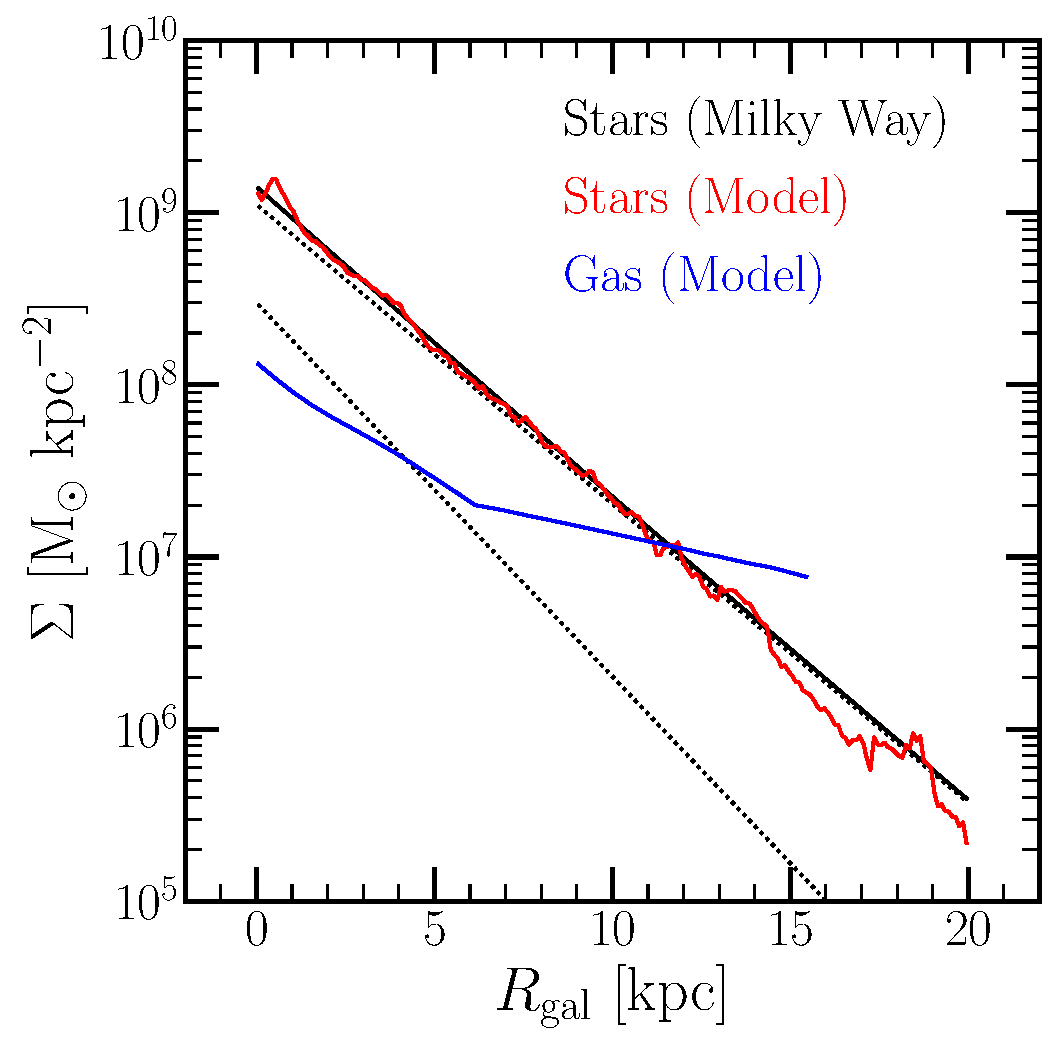
\includegraphics[scale = 0.45]{surface_density_gradient.pdf} 
\caption{The surface density of gas (blue) and stars (red) as predicted by our 
inside-out SFH model. The dotted black line with the higher normalization 
denotes a thin disc profile with scale length $R_t$ = 2.5 kpc; the other 
denotes a thick disc profile with scale length $R_T$ = 2.0 kpc, and a ratio of 
$\Sigma_T/\Sigma_t$ = 0.27 at $R_\text{gal}$ = 0. The black line denotes the 
sum of the two; this is the surface density gradient of the Milky Way as 
reported by~\citet{Bland-Hawthorn2016}, renormalized to imply the same total 
stellar mass within the disc. } 
\label{fig:surface_density} 
\end{figure} 

\begin{itemize} 
	\item As discussed in~\S~\ref{sec:methods:sfhs}, Appendix 
	\ref{sec:normalize_sfh} presents justification of a recipe in which we 
	select a unitless, unnormalized form describing the scaling of the 
	stellar surface density with Galactocentric radius, denoted 
	$g(R_\text{gal})$. Here we adopt the following double exponential form, 
	describing the thin and thick discs of the Milky Way: 
	\begin{equation} 
	g(R_\text{gal}) = e^{-R/R_t} + \frac{\Sigma_T}{\Sigma_t}e^{-R/R_T} 
	\end{equation} 
	where $R_t$ and $R_T$ are the scale radii of the thin and thick discs, 
	respectively, and $\Sigma_T/\Sigma_t$ is the ratio of their surface 
	densities at $R_\text{gal}$ = 0. In this paper, we adopt $R_t$ = 2.5 kpc, 
	$R_T$ = 2.0 kpc, and $\Sigma_T/\Sigma_t$ = 0.27 from the findings of 
	\citet{Bland-Hawthorn2016}. 

	\item Adopt the~\citet{Licquia2015} total stellar mass of 
	$(6.08\pm1.14)\times10^{10}~M_\odot$. We're including bulge star particles 
	in our sample of candidate analogs from~\texttt{h277}, so we model the 
	entire stellar mass as opposed to just the disc, for 
	which~\citet{Licquia2015} found $(5.17\pm1.11)\times10^{10}~M_\odot$. 

	\item Surface density gradient from fiducial model with inside-out SFH, 
	plotted in Fig.~\ref{fig:surface_density} (stars in red and gas in blue). 
	Radial migration indeed didn't change the overall scaling of 
	$\Sigma_\star$ with $R_\text{gal}$ at the radii that we care about in 
	this paper (3 kpc~$\lesssim R_\text{gal} \lesssim$~15 kpc), only 
	introducing scatter. Gas disc appears to be flatten at 
	$R_\text{gal}~\gtrsim$ 6 kpc; this is a consequence of our model for star 
	formation efficiency (see discussion in~\S~\ref{sec:methods:sfe}). Black 
	dotted lines show the individual thin and thick disc components that we 
	adopt from~\citet{Bland-Hawthorn2016}, with the solid line denoting the 
	sum of the two, all re-normalized such that the integral over the surface 
	area of the model Galaxy implies a total stellar mass in agreement with 
	our adopted value from~\citet{Licquia2015}. 
\end{itemize} 

\subsection{Star Formation Efficiency} 
\label{sec:methods:sfe} 

\begin{figure} 
\centering 
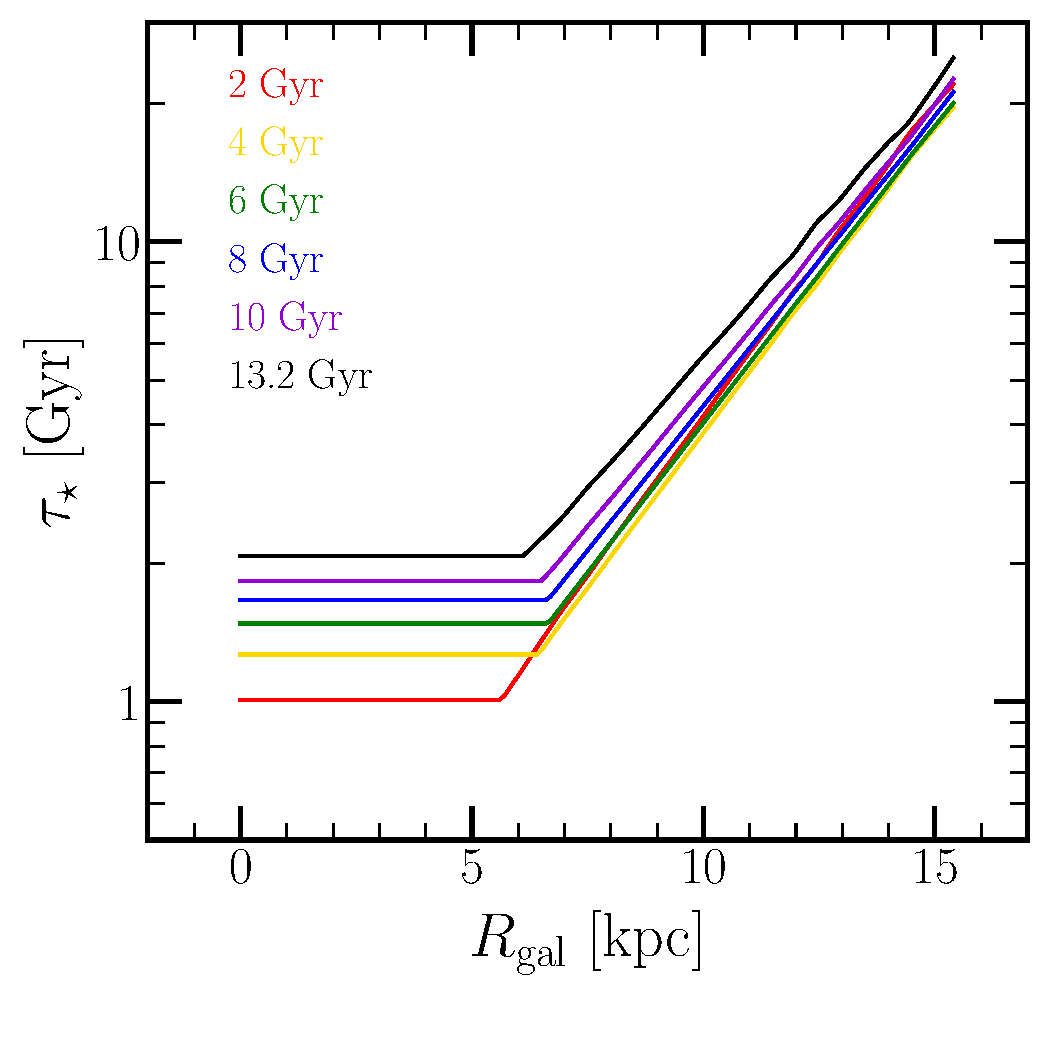
\includegraphics[scale = 0.6]{sfe.pdf} 
\caption{The star formation efficiency timescale $\tau_\star$ as a 
function of Galactocentric radius at simulation times of 2 Gyr (red), 4 Gyr 
(yellow), 6 Gyr (green), 8 Gyr (blue), 10 Gyr (purple), and 12.7 Gyr (i.e. 
the present day, black) predicted by our inside-out SFH model. }
\label{fig:sfe} 
\end{figure} 

\begin{itemize} 
	\item The term ``star formation efficiency'' (SFE) is an overloaded term in 
	the literature. In the star formation/feedback literature, it usually 
	refers to the fraction of a molecular cloud's mass which will eventually 
	be converted into stars. In the chemical evolution literature, however, it 
	usually refers to the inverse timescale relating the star formation rate 
	within some gas reservoir and the mass of the gas reservoir itself: 
	$\tau_\star \equiv \Sigma_\text{gas}/\dot{\Sigma}_\star$. High (Low) 
	values of $\tau_\star$ indicate slow (fast) star formation and thus low 
	(high) SFE; when we refer to SFE here, we're referring to the definition 
	based on this timescale. 
	\begin{itemize} 
		\item Potentially note that this is often referred to as the 
		``depletion time'' in star formation literature, and the 
		\citet{Weinberg2017} definition of depletion 
		time:~$\tau_\text{dep} \equiv \tau_\star/ (1 + \eta - r)$. 
	\end{itemize} 

	\item This is a topic of intense observational inquiry, results of which 
	we review in this section in the interest of obtaining an observationally 
	motivated star formation law. 
	\begin{itemize} 
		\item In practice, many chemical evolution studies adopt a simple 
		power-law for the Kennicutt-Schmidt law relating~$\Sigma_\text{gas}$ 
		and~$\dot{\Sigma}_\star$: $\dot{\Sigma}_\star~\sim 
		\Sigma_\text{gas}^N$, where~\citet{Kennicutt1998} infer 
		$N = 1.4 \pm 0.15$ across a sample of quiescent spiral galaxies and 
		infrared and circumnuclear starbursts.~\citet{delosReyes2019} derive a 
		similar value of $N = 1.41 \pm 0.07$ for local quiescent spiral, 
		dwarf, and low surface brightness galaxies, further demonstrating that 
		much of the observed scatter is intrinsic. 

		\item \citet{Liu2015} demonstrate that the derived value of~$N$ is 
		sensitive to the assumed form of the CO-to-H$_2$ conversion factor 
		($\alpha_\text{CO}$); for fixed~$\alpha_\text{CO}$, they find 
		$N = 1.14 \pm 0.02$, but~$N = 1.60 \pm 0.03$ for a continuously varying 
		$\alpha_\text{CO}$ for a sample of 181 local galaxies with infrared 
		luminosities spanning nearly five orders of magnitude. Much of the 
		uncertainty in the detailed form of the star formation law is likely 
		a consequence of the ongoing debate about~$\alpha_\text{CO}$ (and 
		other mathematical defintions of the conversion factor as well, such 
		as X(CO); see discussion in~\citealp{Kennicutt2012}). 

		\item In extending the~\citet{delosReyes2019} study to the most 
		extreme infrared-luminous and circumnuclear starburst galaxies, 
		\citet{Kennicutt2020} recently found a value of~$N = 1.50 \pm 0.05$. 
		Although they determine that a single power law is a reasonable recipe 
		for models of Galaxy evolution, they demonstrate that there is 
		evidence for significant breaks in both the power-law indeces and the 
		zeropoints. They argue that these breaks are physical in origin, and 
		speculate that it is tied to the transition from a mixed atomic and 
		molecular ISM in normal disc galaxies to a nearly fully molecular ISM 
		in starburst galaxies. A transition to a linear 
		$\dot{\Sigma}_\star-\Sigma_\text{gas}$ relation at a surface density 
		above which the molecular fraction~$f_\text{mol} \approx 1$ is 
		consistent with the finding that star formation proceeds only in the 
		molecular phase~\citep[e.g.][]{Leroy2008, Leroy2013}. 

		\item Consistent with the finding that the intrinsic scatter in the 
		observed~$\dot{\Sigma}_\star-\Sigma_\text{gas}$ relation is physical 
		in origin,~\citet{Ellison2020b} demonstrate that this relation (among 
		other fundamental correlations) shows significant galaxy-to-galaxy 
		variations in both slope and normalization, suggesting that it is not 
		universal between galaxies. \citet{Leroy2013} also find evidence that 
		$\tau_\text{mol}$, the value of $\tau_\star$ for a gas reservoir with 
		$f_\text{mol}$ = 1, is multivalued at fixed $\Sigma_{\text{H}_2}$, 
		suggesting that the rate of star formation is set not only by the 
		density of the gas reservoir, but other environmental parameters as 
		well. 
	\end{itemize} 

	\item Although we acknowledge the collective result that an individual 
	galaxy would not obey the observed, population-averaged 
	$\dot{\Sigma}_\star-\Sigma_\text{gas}$ relation, we decide to adopt 
	such a prescription for our models here. Our motivation for doing so 
	is two-fold. 
	\begin{itemize} 
		\item In practice, we find that our mathematical formalism for 
		$\tau_\star$ does not significantly impact our conclusions; we 
		demonstrate this in Appendix~\ref{sec:sfe_variations}. For this 
		reason, a simple formalism is its own reward for our purposes. 

		\item As discussed in~\S~\ref{sec:methods:sfhs}, we are running 
		\texttt{VICE} in star formation mode; this simply means that we 
		have specified the~\textit{star formation history} of the Galaxy, 
		rather than the infall history or the ISM surface density as 
		functions of simulation time and radius. While many galaxy 
		evolution models use these observed star formation laws to infer 
		the star formation rate from the ISM surface density, here we are 
		doing the inverse - inferring the ISM surface density from the 
		star formation rate. We therefore do not know the properties of 
		the ISM in our simulations a priori, and must resort to simple 
		assumptions anyway. An investigation of more detailed 
		prescriptions for star formation efficiency in models for 
		enrichment in the Milky Way is an interesting which we must 
		reserve for future work due to how we have constructed the 
		simulations presented in this paper. 
	\end{itemize} 

	\item Motivated by these recent results suggesting nuance within the 
	star formation law~\citep{Leroy2013, Ellison2020b, Kennicutt2020}, we 
	implement in our simulations a three-component power-law based on the 
	results presented in~\citet{Krumholz2018}. They construct a turbulence and 
	mass-transfer driven theoretical model for star formation in disc galaxies, 
	and present a comparison of its predictions under a handful of parameter 
	choices to the data from~\citet{Bigiel2010} and~\citet{Leroy2013} (see 
	their Fig. 2). We find that the following by-eye fit is a reasonable 
	description of the aggregate data: 
	\begin{subequations}\begin{align} 
	\dot{\Sigma}_\star &\sim \Sigma_\text{gas}^N \\ 
	N &= \begin{cases} 
	1.0 & (\Sigma_\text{gas} \geq 2\times10^7~\text{M}_\odot~\text{kpc}^{-2}) 
	\\ 
	3.6 & (5\times10^6~\text{M}_\odot~\text{kpc}^{-2} \leq \Sigma_\text{gas} 
		\leq 2\times10^7~\text{M}_\odot~\text{kpc}^{-2}) 
	\\ 
	1.7 & (\Sigma_\text{gas} \leq 5\times10^6~\text{M}_\odot~\text{kpc}^{-2}) 
	\end{cases} 
	\label{eq:ks_law} 
	\end{align}\end{subequations} 

	\item The apparent linearity of the relationship above~$\sim2\times10^7$ 
	M$_\odot$ kpc$^{-2}$ suggests that in this regime, star formation is 
	proceeding at the fastest possible rate, and that $\tau_\star$ = 
	$\Sigma_\text{gas}/\dot{\Sigma}_\star$ = constant. The results of 
	\citet{Leroy2008, Leroy2013} and~\citet{Kennicutt2020} would suggest that 
	this is the regime in which~$f_\text{mol}$ = 1. We therefore adopt the 
	assumptions that $f_\text{mol}$ is unity above an ISM surface density of 
	$\Sigma_\text{gas} = 2\times10^7$~M$_\odot$~kpc$^{-2}$ and that 
	$\tau_\star$ assumes that value of $\tau_\text{mol}$ at these densities, 
	increasing with decreasing~$f_\text{mol}$. 

	\item With the formulation of the Kennicutt-Schmidt Law described by 
	equation~\refp{eq:ks_law} and the mathematical definition 
	$\tau_\star \equiv \Sigma_\text{gas}/\dot{\Sigma}_\star$, we can derive 
	$\tau_\star-\Sigma_\text{gas}$ or $\tau_\star-\dot{\Sigma}_\star$ 
	relationships as required by~\texttt{VICE}. With~$\tau_\star$ = 
	$\tau_\text{mol}$ at~$\Sigma_\text{gas}~\geq~2\times10^7$~M$_\odot$ 
	kpc$^{-2}$ setting the overall normalization, the following describes the 
	resultant~$\tau_\star-\Sigma_\text{gas}$ relationship: 
	\begin{equation}
	\tau_\star = \begin{cases} 
	\tau_\text{mol} & (\Sigma_\text{gas} \geq \Sigma_\text{gas,1}) 
	\\ 
	\tau_\text{mol} \left(\frac{\Sigma_\text{gas}}{\Sigma_\text{gas,1}}
		\right)^{\beta_1} & (\Sigma_\text{gas,2} \leq \Sigma_\text{gas} \leq 
		\Sigma_\text{gas,1}) 
	\\ 
	\tau_\text{mol} \left(\frac{\Sigma_\text{gas,2}}{\Sigma_\text{gas,1}}
		\right)^{\beta_1} \left(\frac{\Sigma_\text{gas}}{\Sigma_\text{gas,2}}
		\right)^{\beta_2} & (\Sigma_\text{gas} \leq \Sigma_\text{gas,2}) 
	\end{cases} 
	\end{equation} 
	where we adopt~$\Sigma_\text{gas,1} = 2\times10^7$ M$_\odot$ kpc$^{-2}$, 
	$\Sigma_\text{gas,2} = 5\times10^6$ M$_\odot$ kpc$^{-2}$,~$\beta_1$ = 
	-2.6, and~$\beta_2$ = -0.7\footnote{
		$\beta = 1 - N$, where N is the power-law index of the 
		$\dot{\Sigma}_\star-\Sigma_\text{gas}$ relationship. 
	}. The additional factor of 
	$(\Sigma_\text{gas,2}/\Sigma_\text{gas,1})^{\beta_1}$ simply ensures that 
	this formalism is piecewise-continuous. 

	\item Based on the observed Kennicutt-Schmidt relation at different 
	redshifts,~\citet{Tacconi2018} suggest that~$\tau_\text{mol}$ should 
	scale with redshift~$z$ and the deviation from the star forming main 
	sequence~$\delta\text{MS}$ via~$\tau_\text{mol} \propto (1 + z)^{-0.6} 
	\delta\text{MS}^{-0.44}$. We don't take into account the effect of 
	$\delta\text{MS}$ in our models, but we do investigate the redshift 
	dependence. A reasonable approximation to the $t-z$ relation out 
	to~$z \approx$~3 assuming typical~$\Lambda$CDM cosmology is given by: 
	\begin{equation} 
	\frac{t}{t_0} \approx (1 + z)^{-5/4} 
	\end{equation} 
	where $t_0$ is the present-day age of the universe, and $t$ is not 
	simulation time but the age of the universe at any given redshift. 
	Plugging this relation into the~\citet{Tacconi2018} scaling yields the 
	following time-dependence for~$\tau_\text{mol}$: 
	\begin{equation} 
	\tau_\text{mol} = \tau_{\text{mol},0}(t/t_0)^{12/25} \approx 
	\tau_{\text{mol},0}(t/t_0)^{1/2} 
	\end{equation} 
	where $\tau_{\text{mol},0}$ is simply $\tau_\text{mol}$ at the 
	present day. We generalize this formula to the following form: 
	\begin{equation} 
	\tau_\text{mol} = \tau_{\text{mol},0}(t/t_0)^\gamma 
	\end{equation} 
	In this paper we present simulations which adopt~$\tau_{\text{mol},0}$ 
	= 2 Gyr~\citep{Leroy2008, Leroy2013, Tacconi2018} and~$\gamma$~= 1/2 based 
	on this argument. We have also ran simulations which adopt 
	$\tau_{\text{mol},0}$ = 1 Gyr and~$\gamma$~= 0 (a time-independent 
	$\tau_{\text{mol}}$), and found similar results. 

	\item Fig.~\ref{fig:sfe} shows $\tau_\star$ as a function of $R_\text{gal}$ 
	at six different time stamps predicted by our fiducial, inside-out SFH 
	model. Wherever~$\tau_\star$ is at its minimum value is where the ISM in 
	that annulus is fully molecular. 
	\begin{itemize} 
		\item In the fiducial inside-out model, the molecular fraction is near 
		unity out to~$R_\text{gal} \approx$~6 kpc at all times. 

		\item From the actual value of $\tau_\star$ at a given radius and time 
		and the assumed $\tau_\text{mol}$ in the model, we can derive the 
		model predicted molecular fractions within the disk via 
		$f_\text{mol} = \tau_\text{mol}/\tau_\star$, then subsequently the 
		HI + HII and H$_2$ masses from $f_\text{mol}$ and the total gas supply 
		after subtracting 27\% to account for helium. 

		\item These post-processing calculations suggest that our fiducial 
		inside-out model predicts an HI + HII mass of~$5.54\times10^9$ 
		M$_\odot$ and an H$_2$ mass of~$7.14\times10^9$~M$_\odot$ within 
		$R_\text{gal}$ = 20 kpc, the maximum radius in our model. This 
		predicts a total H mass of~$1.27\times10^{10}$~M$_\odot$, and a total 
		ISM mass of~$1.74\times10^{10}$~M$_\odot$ after adding 27\% back to 
		account for helium. This yields a global molecular fraction of 
		$f_\text{mol}$ = H$_2$ / (HI + HII + H$_2$) = 56\%. In comparison with 
		observed results, this is an overprediction of~$f_\text{mol}$; 
		\citet{Kalberla2009} report a value of~$8\times10^9$ and 
		$2.5\times10^9$~M$_\odot$ for the HI and H$_2$ masses within 60 kpc, 
		the bulk of which is in the disk. They report an additional 
		$\sim2\times10^9$~M$_\odot$ in the warm ionized medium (HII). 
		\citet{Heyer2015} argue for a lower H$_2$ mass of~$1\times10^9$ 
		M$_\odot$. Our fiducial model is over-predicting the H$_2$ mass by a 
		factor of~$\sim$3 and under-predicting the HI + HII mass by a factor 
		of~$\sim$2. 

		\item Whatever the source of this discrepancy may be, we present in 
		Appendix~\ref{sec:sfe_variations} a variation of our fiducial model 
		with a significantly different assumption about~$\tau_\star$, and 
		demonstrate that this decision does not impact our general 
		conclusions. We reserve discussion on potential sources of this 
		discrepancy to Appendix~\ref{sec:sfe_variations} as well. {\color{red} 
		This discussion may move back to this section, but I had some ideas 
		on this, so I moved stuff later so that the methods section doesn't 
		get lost in minutia. }
	\end{itemize} 
\end{itemize} 

\subsection{Summary} 
\label{sec:methods:summary} 

\begin{itemize} 
	\item In summary, our fiducial model has an inside-out SFH (see~\S 
	\ref{sec:methods:sfhs}) with the star formation law as described in~\S 
	\ref{sec:methods:sfe}, radial migration the proceeds according to the 
	diffusion model (see~\S~\ref{sec:methods:migration}), and yields and 
	outflows as described in~\S~\ref{sec:methods:yields}. 

	\item We have also conducted runs with the three other SFHs, the three 
	other migration prescriptions, and the three other SFE prescriptions - a 
	total of 64 simulations, as well as a variety of other test cases. In this 
	paper, we present results wherever the model predictions are sensitive to 
	the assumptions. However, in general the differences can be understood 
	with only the variations in star formation history and the qualitative 
	notion that many stars have moved beyond their birth radius. 

	\item To ensure that resolution does not affect our results, we ran the 
	same set of models with~$n$ = 2 stellar populations per zone per 
	timestep, and found similar predictions. 
\end{itemize} 

\section{Metallicity Space} 
\label{sec:metallicity_space} 

\begin{figure*} 
\centering 
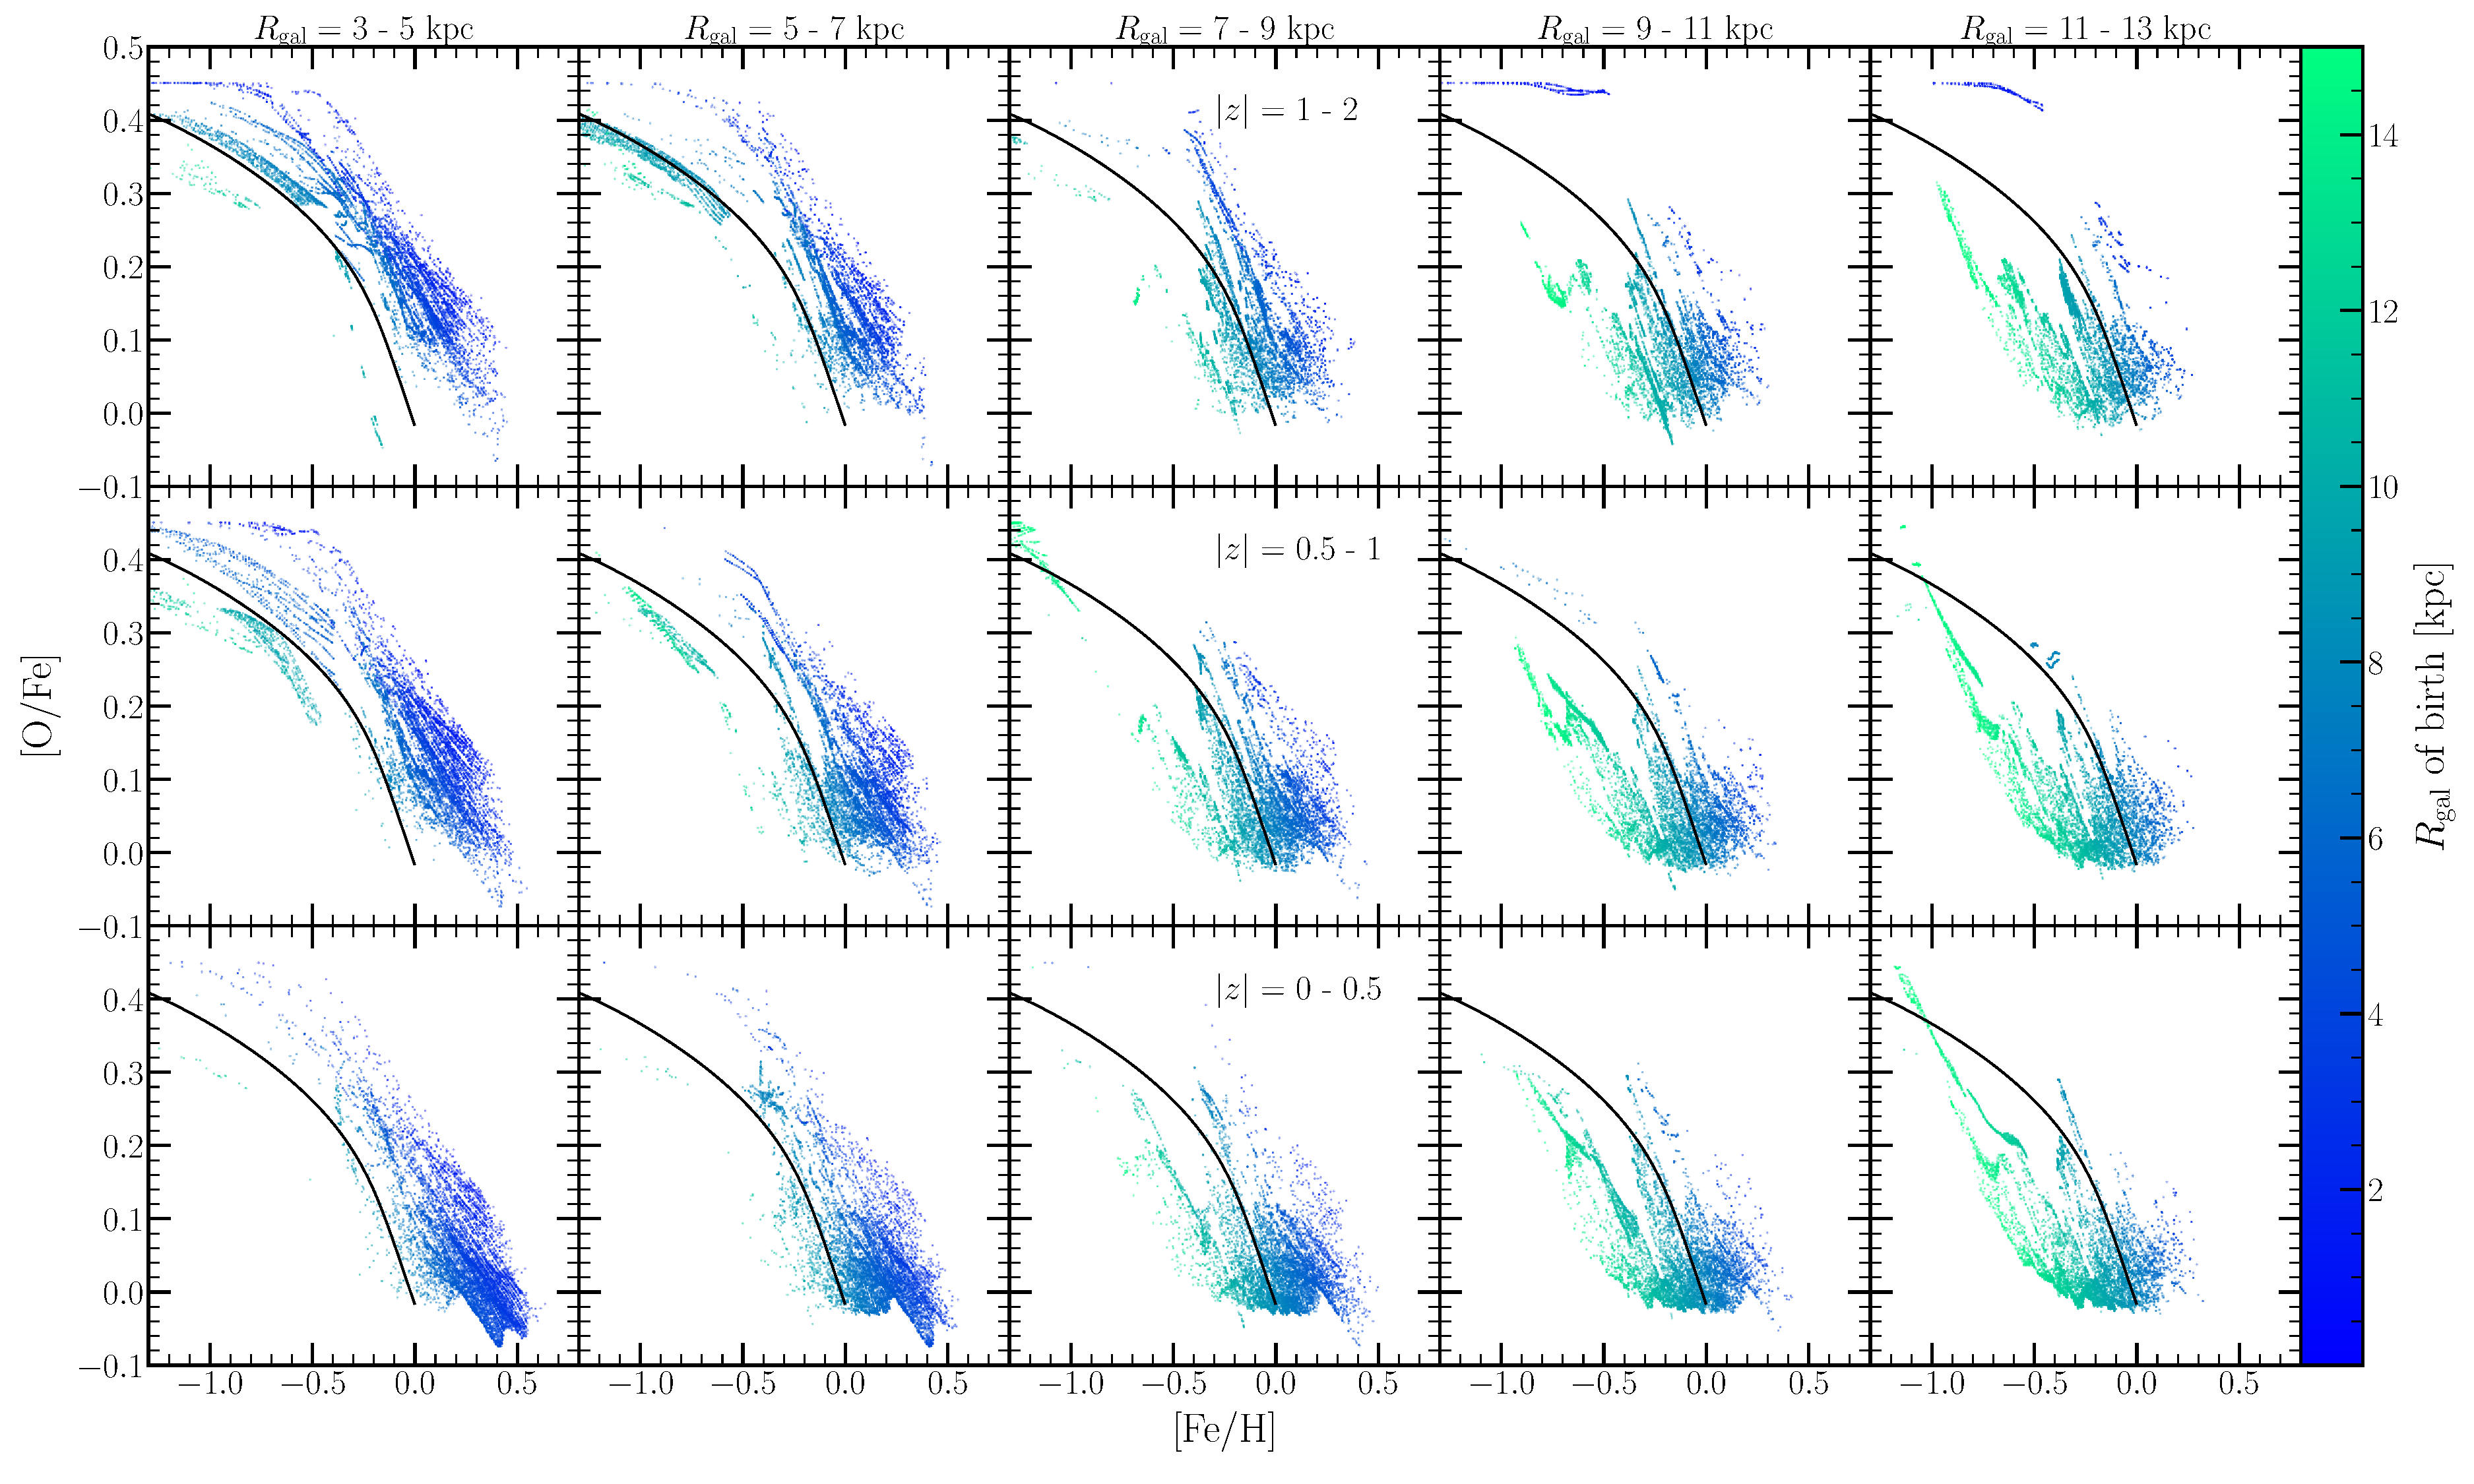
\includegraphics[scale = 0.28]{ofe_feh_densitymap.pdf} 
\caption{[O/Fe]-[Fe/H] diagrams for 15 galactic regions spanning five bins in 
$R_\text{gal}$ and~$\left|z\right|$. Each region has its own panel, with radial 
bins shown in columns denoted at the top of the figure, and with 
$\left|z\right|$ bins shown in rows denoted in text in the middle column. In 
each panel, we plot $N$ = 10,000 points sampled from our simulated 
stellar populations in each region predicted by our inside-out SFH, where the 
probability of sampling is proportional to the present-day mass of each stellar 
population. In all panels points are color-coded according to the 
Galactocentric radius of birth of the stellar population. For reference, we 
plot in a solid black line in all panels the gas-phase [O/Fe]-[Fe/H] track 
predicted by the same SFH in the $R_\text{gal}$ = 8 kpc annulus, but with the 
post-processing migration model; this curve is the same in all panels. }
\label{fig:ofe_feh_diagram} 
\end{figure*} 

\begin{figure*} 
\centering 
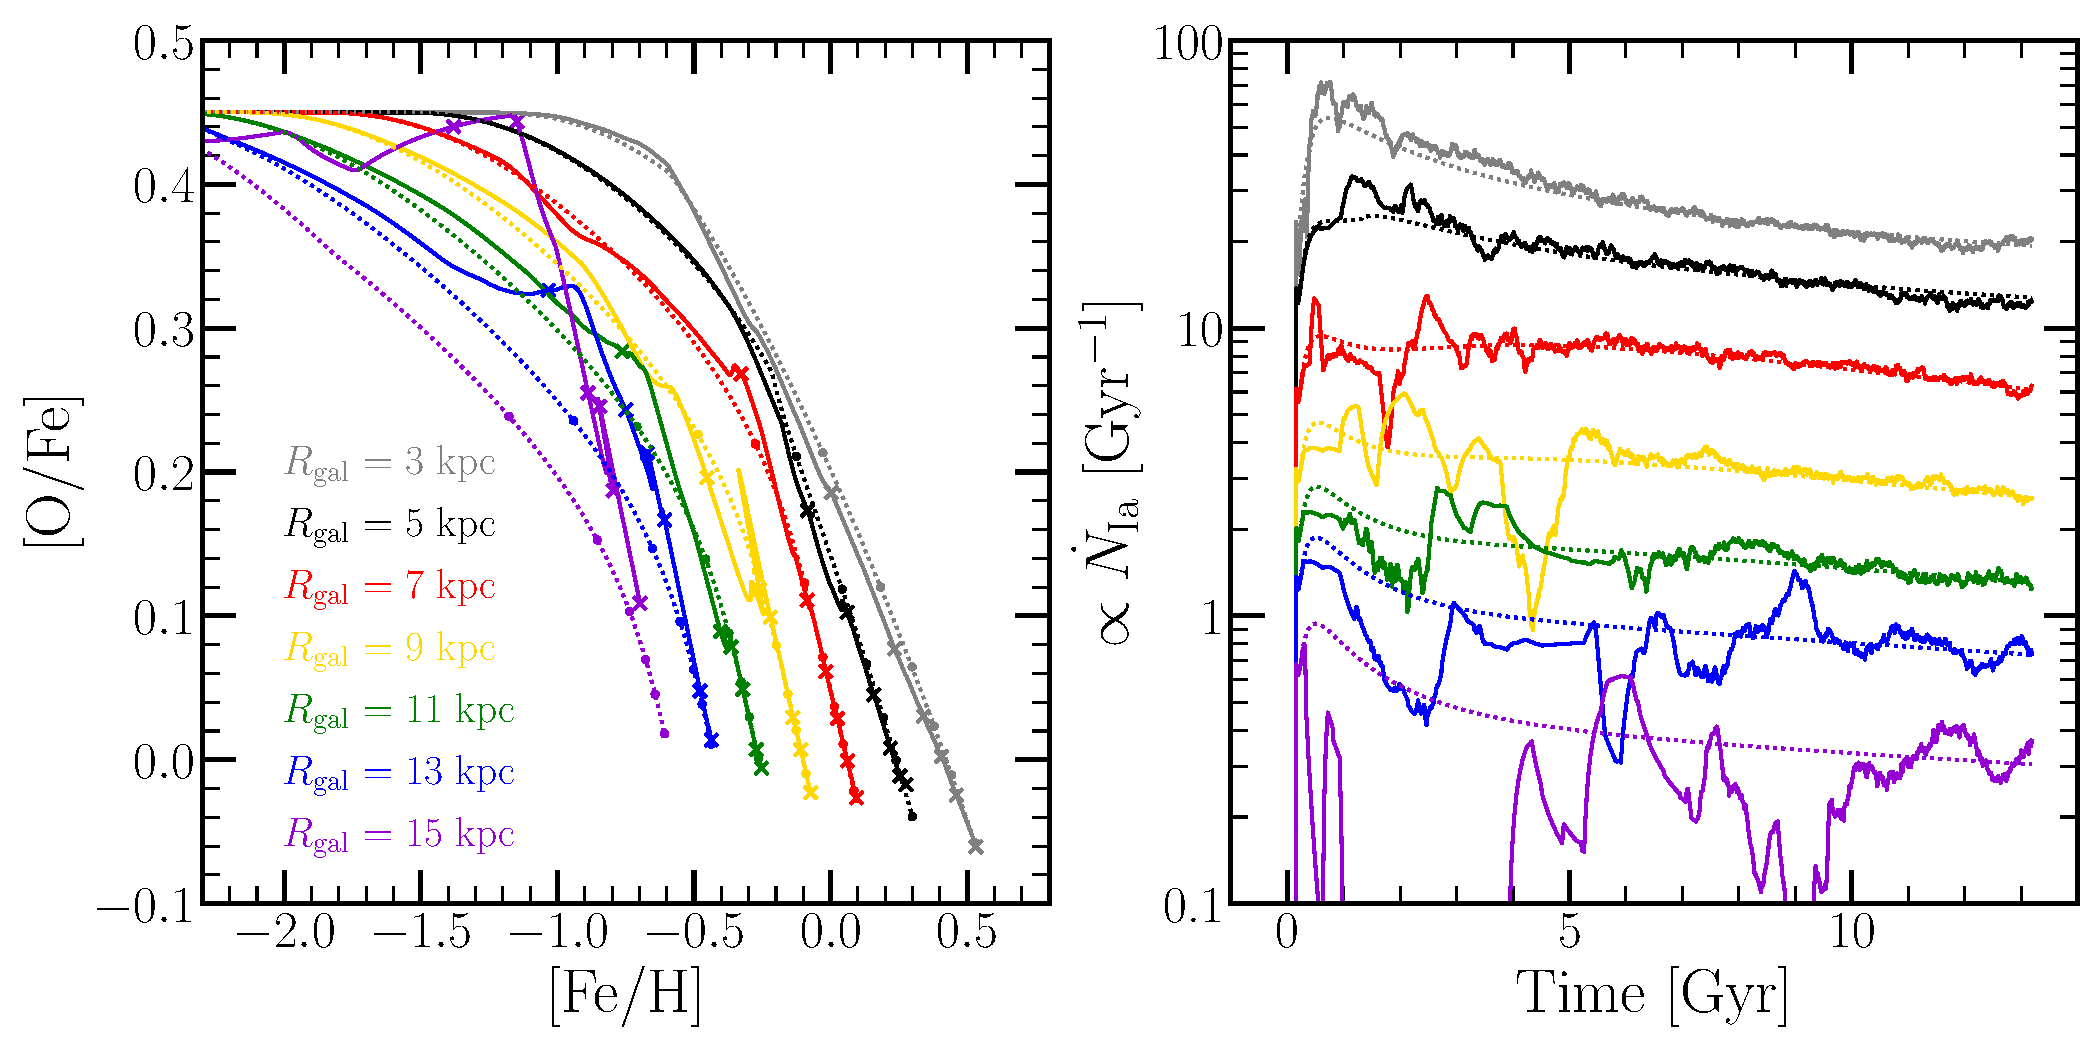
\includegraphics[scale = 0.42]{tracks.pdf} 
\caption{\textbf{Left}: Gas phase evolutionary tracks in the [O/Fe]-[Fe/H] 
plane for our inside-out SFH with either post-processing (dotted lines) or 
diffusion (solid lines) migration models. We plot tracks for seven annuli, 
color-coded according to their Galactocentric radius and denoted by the legend 
in the lower-left. We mark simulation times of 2, 4, 6, 8, 10, and 12.7 Gyr in 
X's for the diffusion model and points for the post-processing model. 
\textbf{Right}: The proxy for the SN Ia rate defined in equation 
\refp{eq:ia_rate_proxy} as a function of simulation time for the same annuli 
as in the left-hand panel. We multiply rates at each radii here by various 
prefactors to improve of clarity. }
\label{fig:tracks} 
\end{figure*} 

\begin{itemize} 
	\item Fig.~\ref{fig:ofe_feh_diagram} shows a scatter plot of 10,000 
	randomly sampled stellar populations in five bins of $R_\text{gal}$ and 
	three bins of $\left|z\right|$ ($R_\text{gal}$ = 3 - 5 kpc, 5 - 7 kpc, 
	7 - 9 kpc, 9 - 11 kpc, and 11 - 13 kpc; $\left|z\right|$ = 0 - 0.5 kpc, 
	0.5 - 1 kpc, and 1 - 2 kpc). These are the same bins and same scheme for 
	organizing the panels as in Fig. 4 of~\citet{Hayden2015}. 

	\item The width of the low-$\alpha$ sequence predicted by the model comes 
	from radial migration. Though this is somewhat guaranteed by our model 
	in choosing equilibrium abundances that reflect a realistic metallicity 
	gradient, it is in good agreement with~\citet{Schoenrich2009} and 
	\citet{Nidever2014}. 

	\item The low-$\alpha$ sequence shifts from a high [Fe/H] locus at small 
	$R_\text{gal}$ to low [Fe/H] at high~$R_\text{gal}$, in agreement with the 
	observed distributions in APOGEE presented in~\citet{Hayden2015}. 

	\item High-$\alpha$ stars are most prevalent at low~$R_\text{gal}$ and 
	high~$\left|z\right|$, and conversely for the low-$\alpha$ stars, also 
	in agreement with~\citet{Hayden2015}. 
	\begin{itemize} 
		\item Similar results are found for different SFHs. This suggests that 
		this observed result is a natural consequence of stellar migration. 

		\item Only minor difference worth noting is that the starburst models 
		predict a slightly higher characteristic [O/Fe] ($\sim$+0.1) for the 
		low-$\alpha$ sequence. This is a natural consequence of the starburst 
		producing young,~$\alpha$-enhanced stars~\citep{Johnson2020}. 
	\end{itemize} 

	\item Left-hand panel of Fig.~\ref{fig:tracks} compares the tracks 
	predicted by our fiducial, inside-out SFH assuming diffusion migration 
	(sudden) versus post-processing (dotted) for the gas-phase of a handful of 
	radii denoted by the legend. Predicted [O/Fe]-[Fe/H] tracks for the 
	diffusion model show significant deviations from the post-processing 
	model. We demonstrate here that this is due to variability in the SN Ia 
	rate induced by the time-dependent radial migration of the diffusion 
	model. Simulation times of 2, 4, 6, 8, 10, and 12.7 Gyr shown in points 
	and X's for the two models. 

	\begin{itemize} 
		\item For each zone,~\texttt{VICE} provides in its outputs the rates 
		of infall and star formation, the mass of the ISM, and the relevant 
		abundance information for each element along with the associated 
		MDFs at the final timestep. To determine the SN Ia rates, we therefore 
		have to approximate from the output. 

		\item The time-derivative of the mass of Fe in a given annulus is 
		given by: 
		\begin{equation}
		\dot{M}_\text{Fe} \approx y_\text{Fe}^\text{CC}\dot{M}_\star + 
		y_\text{Fe}^\text{Ia}\langle\dot{M}_\star\rangle_\text{Ia} - 
		\frac{M_\text{Fe}}{M_g}\dot{M}_\star(1 + \eta(R_\text{gal}) - r) 
		\end{equation} 
		where this is an approximation because in detail, there is a small 
		contribution from AGB stars, and the recycling in the simulation is 
		done continuously, whereas here we simply take $r \approx$ 0.4 
		(appropriate for a~\citetalias{Kroupa2001} IMF; 
		\citealp{Weinberg2017}). This equation can be derived from the 
		\citet{Weinberg2017} analytic models assuming CCSN and SN Ia 
		enrichment for Fe with instantaneous recycling of previously produced 
		Fe.~\texttt{VICE}'s science documentation could also be referenced 
		here; it has a nice detailed section on its treatment of each term in 
		handling enrichment rates \footnote{
			\url{https://vice-astro.readthedocs.io/en/latest/science_documentation/enrichment/index.html}
		}. 
		Rearranging this for the term describing the rate of injection due to 
		SNe Ia events, and normalizing by $M_\text{Fe}$ yields the following 
		proxy with units of frequency: 
		\begin{equation} 
		\frac{
			y_\text{Fe}^\text{Ia}\langle\dot{M}_\star\rangle_\text{Ia}
		}{
			M_\text{Fe} 
		} \approx 
		\frac{\dot{M}_\text{Fe}}{M_\text{Fe}} - y_\text{Fe}^\text{CC}\frac{
			\dot{M}_\star 
		}{
			M_\text{Fe} 
		} + \frac{\dot{M}_\star}{M_g}(1 + \eta(R_\text{gal}) - r) 
		\label{eq:ia_rate_proxy} 
		\end{equation} 
		This term on the left-hand side can be substituted with 
		$m_\text{Fe}^\text{Ia}\dot{N}_\text{Ia}/M_\text{Fe}$, where 
		$m_\text{Fe}^\text{Ia}$ is the average mass of Fe produced by a single 
		SN Ia event, and $\dot{N}_\text{Ia}$ is the SN Ia rate itself. For 
		this reason, this equation constitutes a straight-forward proxy for 
		the SN Ia rate at any given time. 

		\item This proxy is plotted against simulation time in the right-hand 
		panel of Fig.~\ref{fig:tracks} for the same annuli as in the left-hand 
		panel, with multiplicative factors added for visual clarity, diffusion 
		model again shown in solid lines, post-processing in dotted lines. 
		Whenever and wherever there is a deficit in SN Ia events relative to 
		the post-processing model, the diffusion model tends toward higher 
		[O/Fe] values than the post-processing scenario. Conversely, lower 
		[O/Fe] for an excess in SN Ia events. 

		\item SN Ia rates show high-amplitude variability on Gyr timescales, 
		with low-amplitude white-noise on shorter timescales, potentially 
		introduced at least in part by our discretization of the disc into 
		annuli and the evolution into timesteps. The log-scaled y-axis makes 
		it clear that the fractional amplitude is higher near the outskirts 
		of the disc. This makes physical sense, because the stellar number 
		density is much lower there, and as such would be much more 
		susceptible to sampling noise - that is, a single star migrating 
		has a larger fractional impact on the stellar density and thus the 
		supernova rates at large radii than small radii. 
	\end{itemize} 

	\item This is proof of concept that radial migration of nucleosynthetic 
	yields can occur alongside stellar migration for delayed sources. In 
	principle, it is reasonable to expect similar effects for s-process 
	elements like carbon, nitrogen, strontium, yttrium, zirconium, etc. which 
	are produced in AGB stars, though we do not investigate the impact for 
	these elements here. 

	\item In the literature, it's not uncommon to adopt tracks for different 
	Galactocentric radii in the [O/Fe]-[Fe/H] plane to infer birth radii for 
	observed stars. While an additional dimension such as age could mitigate 
	these potential issues, we caution against inferring birth radii in this 
	manner, because the tracks themselves appear to be sensitive to the 
	dynamical history of the Galaxy. Based on the left-hand panel of Fig. 
	\ref{fig:tracks}, this effect could bias the inferred radii by many kpc. 
	This however doesn't appear to be an issue for the low-$\alpha$ sequence, 
	where the width of the [Fe/H] distribution appears to come from migration 
	itself, as it did in~\citet{Schoenrich2009} and~\citet{Nidever2014}. 
	We therefore recommend that such a technique be restricted to 
	[O/Fe]~$\lesssim$+0.1 stars. 

	\item Demonstrate in~\S~\ref{sec:age_alpha:migration} that this is a means 
	with which to form $\alpha$-rich and $\alpha$-poor stars - or rather 
	Fe-poor and Fe-rich, respectively. 
\end{itemize} 


\section{Metallicity Gradient} 
\label{sec:metallicity_gradient} 

\begin{figure*} 
\centering 
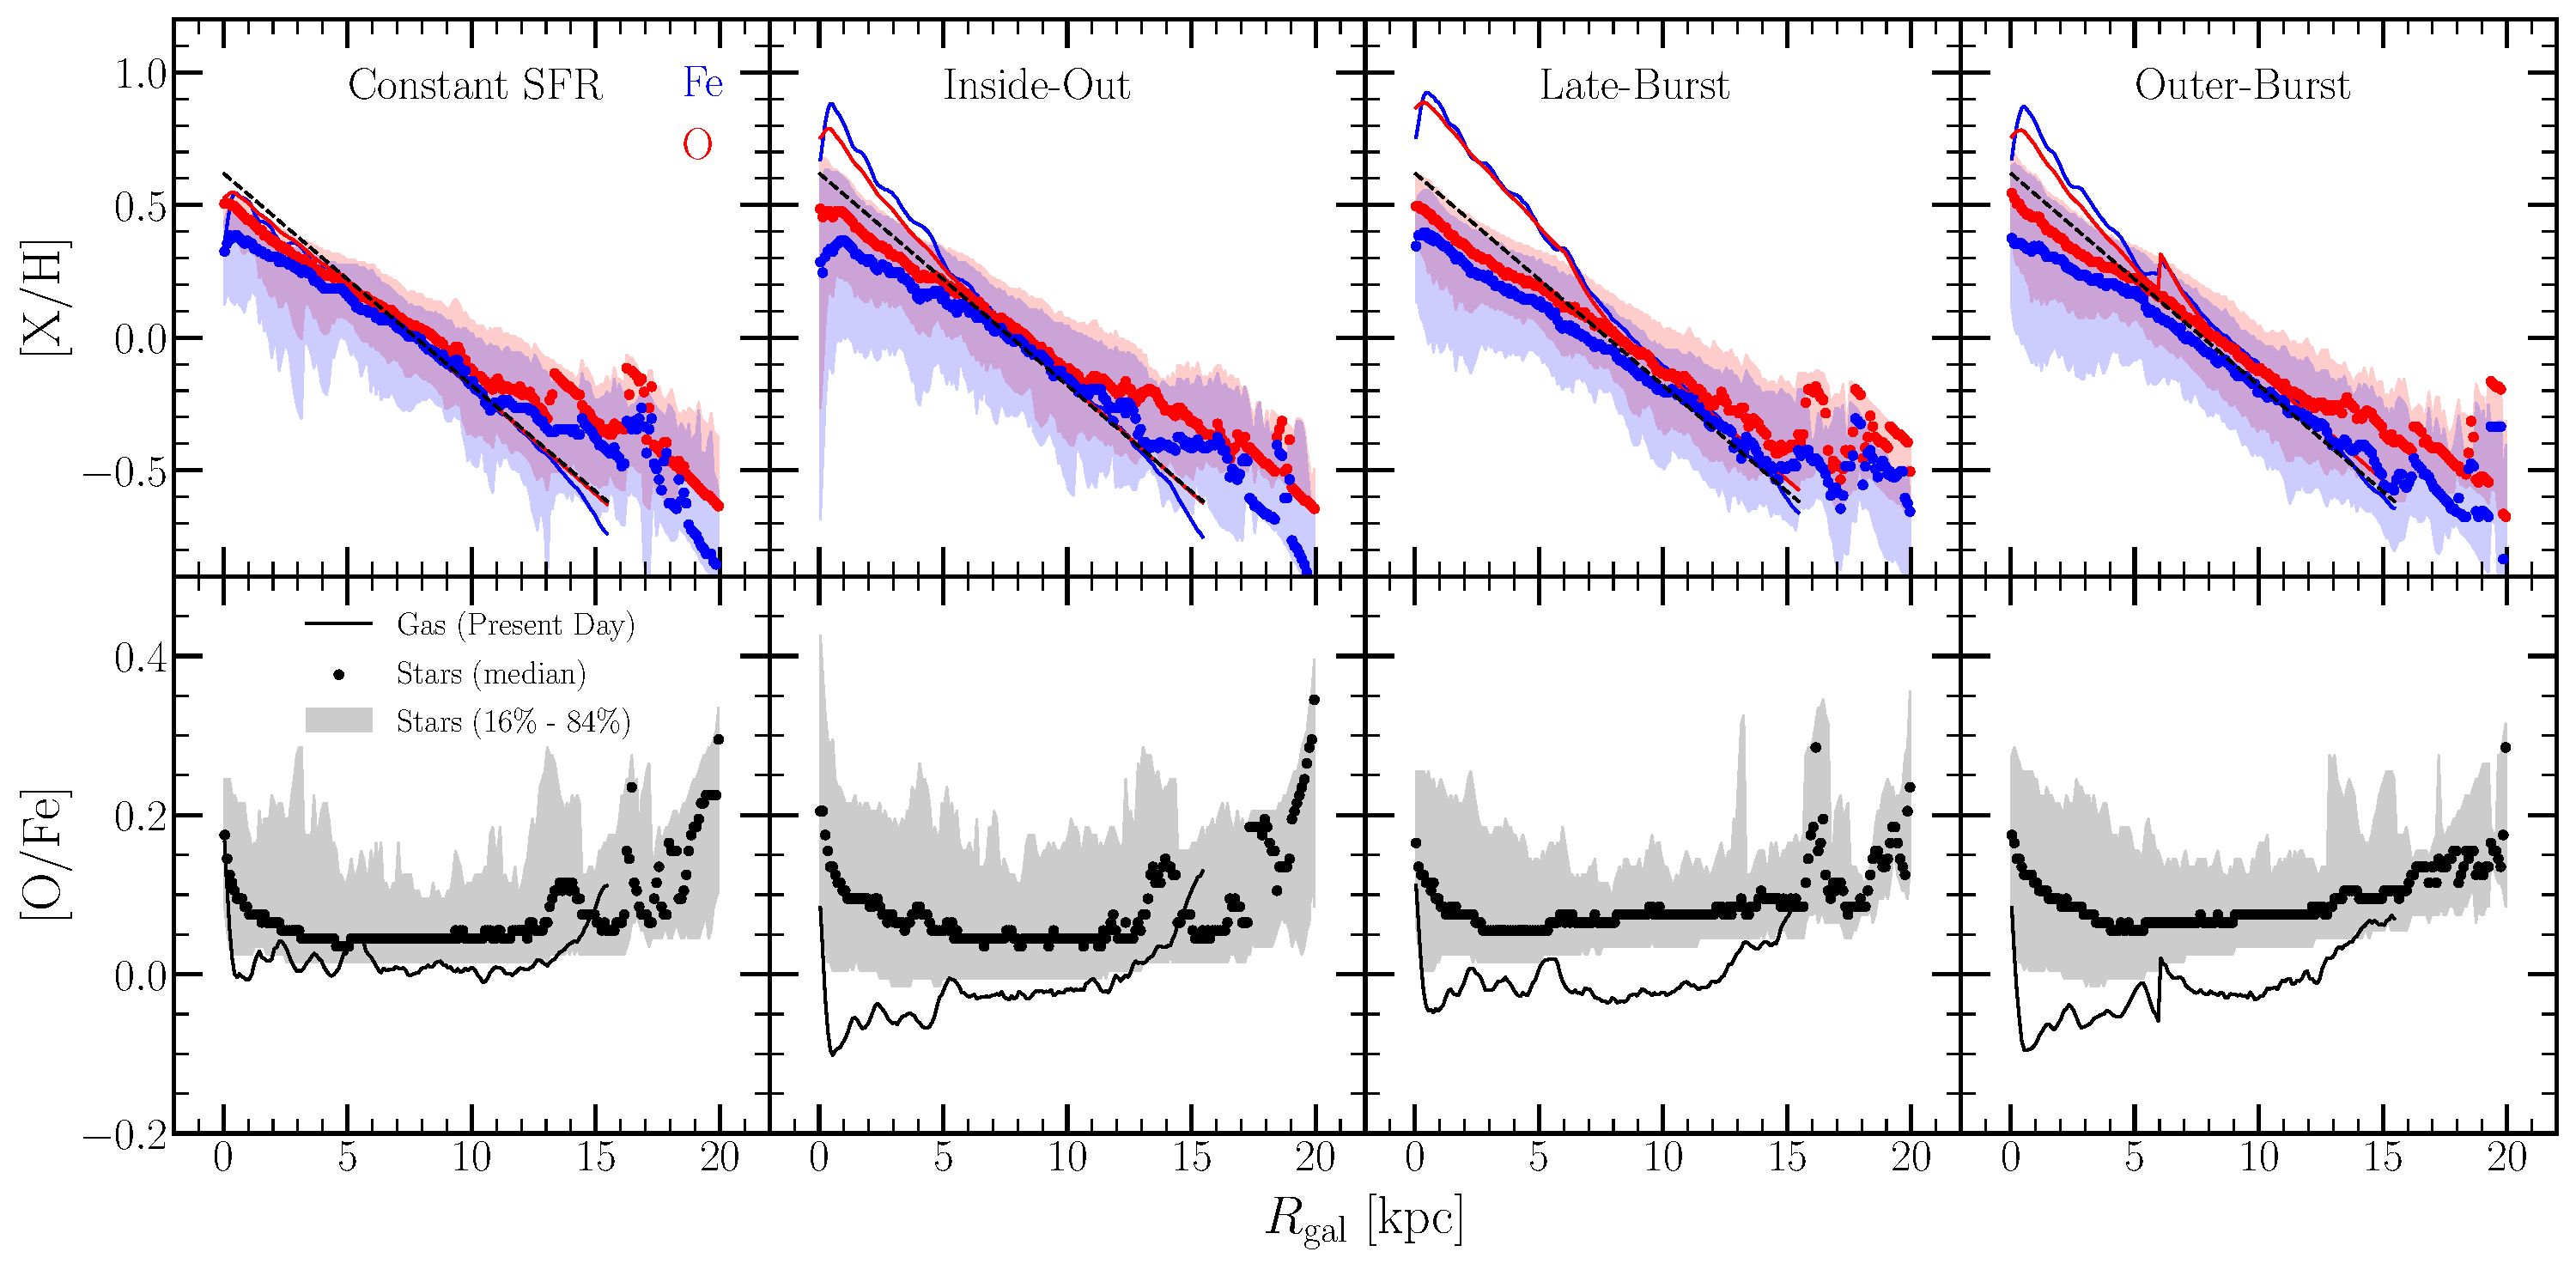
\includegraphics[scale = 0.32]{metallicity_gradient.pdf} 
\caption{Radial abundance gradients in [O/H] (top, red) [Fe/H] (top, blue), 
and [O/Fe] (bottom) for our four fiducial SFHs - constant (far left), 
inside-out (left-middle), late-burst (right-middle), and outer-burst (far 
right). We plot the gas phase abundance at the present day as a function of 
Galactocentric radius in solid lines. Stars denote the mode of the stellar 
MDF of the 100-pc width annulus at a given radius, with shaded regions 
marking the 16th and 84th percentiles thereof. Black lines in the top panels 
denote our target [$\alpha$/H] gradient of mode([$\alpha$/H]) = +0.3 at 
$R_\text{gal}$ = 4 kpc with a slope of -0.08 kpc$^{-1}$. } 
\label{fig:metallicity_gradient} 
\end{figure*} 

\begin{itemize} 
	\item Scaling of $\eta$ with $R_\text{gal}$ based on reproducing the 
	observed mode([$\alpha$/H])-$R_\text{gal}$ trend, neglecting radial 
	migration (see~\S~\ref{sec:methods:yields}). The target gradient is 
	shown in a solid black line in the top panels of Fig. 
	\ref{fig:metallicity_gradient}. 

	\item In the top panels, red and blue stars show the mode O and Fe 
	abundances in each annulus, and the shaded region shows the 16th and 
	84th percentiles of the MDF in that zone. Solid lines show the gas-phase 
	abundance gradient at the present day. Bottom panels show the same thing 
	for [O/Fe]. 

	\item Gradient is indeed recovered in [O/H], and radial migration appears 
	to only induce scatter. While Fe did not enter into our procedure for 
	setting the metallicity gradient, the model predicts a similar gradient 
	for [Fe/H]. 

	\item Clear that the MDF shows a metal-rich mode and skew-negative shape 
	in the inner galaxy for both O and Fe. $\alpha$-enhanced tail there as 
	well. We demonstrate in~\S~\ref{sec:metallicity_gradient} that the MDF 
	does shift to skew-positive in the outer galaxy, though this isn't as 
	visually obvious from this plot due to the scatter in the mode at these 
	radii. 

	\item Details of the [O/Fe] gradient seem to be sensitive to differences 
	in our SFHs, especially in the inner galaxy. 

	\item Constant SFH is the only model in which the present-day gas phase 
	gradient matches the stellar gradient at all radii. In remaining models, 
	the present-day gas-phase abundance is above the majority of the stars 
	because the star formation rate has decreased. We therefore expect 
	observational studies of abundance gradients to differ noticeably between 
	gas and stars. 

	\item Stellar gradient is somewhat shallower in the late-burst model; this 
	is because of the dilution associated with the starburst. Target gradient 
	represents the equilibrium abundance at all radii, and we deliberately 
	perturbed it from equilibrium, so any deviations from the expectation are 
	a consequence of that. 

	\item Late-burst model has super-equilibrium gas phase abundance at the 
	present day. Can be seen by comparing it to the outer-burst model's 
	gas phase gradient and seeing that it has a break at $R_\text{gal}$ = 6 
	kpc, the threshold for the late starburst in this model. This is a 
	consequence of the starburst as well - in infall driven starbursts, 
	re-enrichment can produce super-equilibrium abundances which then decay 
	back to the equilibrium abundance as the star formation rate declines 
	\citep{Johnson2020}. 
\end{itemize} 



% \subsection{The Observed Sample} 
% \label{sec:methods:observed_sample} 

% \begin{itemize} 
% 	\item For the age-metallicity and age-[$\alpha$/Fe] relations, we compare 
% 	to the results of~\citet{Feuillet2019}. Also compared 
% 	to~\citet{Feuillet2018}, the primary difference being that solar 
% 	metallicity stars are found to be considerably younger in the earlier 
% 	study. 

% 	\item While we make use of DR16 in comparing our predicted MDFs to the 
% 	APOGEE data,~\citet{Feuillet2018} and~\citet{Feuillet2019} made use of the 
% 	14th data release (DR14;~\citealp{Abolfathi2014}). We don't expect this 
% 	slight difference to impact our conclusions. 
% \end{itemize} 

\section{Metallicity Distribution Functions} 
\label{sec:mdfs} 

\subsection{[O/H] and [Fe/H]} 
\label{sec:mdfs:oh_feh} 

\begin{itemize} 
	\item MDFs in bins of Galactocentric radius are a fundamental observable 
	to test the validity of any chemical evolution model. In this section we 
	compare our predicted MDFs to those observed in the 16th data release 
	(DR16;~\citealp{Ahumada2020}) of the Apache Point Observatory Galaxy 
	Evolution Experiment (APOGEE;~\citealp{Majewski2017}). The data is 
	reduced using the APOGEE Stellar Parameters and Chemical Abundances 
	Pipeline (ASPCAP;~\citealp{Holtzman2015, GarciaPerez2016}). For further 
	details on the APOGEE survey, a brief summary can be found in~\S~2 of 
	\citet{Weinberg2019}. 
	% A part of the Sloan 
	% Digital Sky Survey (SDSS), APOGEE data is collected with a 300-fiber 
	% H-band spectrograph~\citep{Wilson2020} on the 2.5-meter Sloan Foundation 
	% telescope at Apache Point Observatory~\citep{Gunn2006}. The APOGEE sample 
	% largely consists of evolved stars with 2MASS~\citep{Skrutskie2006} 
	% magnitudes in the range 7 < $H$ < 13.8 sampled on a grid of sightlines 
	% at Galactic latitudes $b$ = -8$^\circ$, -4$^\circ$, 0$^\circ$, +4$^\circ$, 
	% and +8$^\circ$ and a wide range of longitudes. \citet{Nidever2015} 
	% describes the data processing pipeline for APOGEE, providing the input to 
	% the APOGEE Stellar Parameters and Chemical Abundances Pipeline (ASPCAP; 
	% \citealp{Holtzman2015,GarciaPerez2016}). ASPCAP simultaneously fits 
	% elemental abundances, effective temperatures, and surface gravities using a 
	% grid of synthetic spectra predicted by 1-dimensional stellar atmospheric 
	% models assuming local thermodynamic equilibrium~\citep{Meszaros2012, 
	% Zamora2015} and the spectral line list provided in~\citep{Shetrone2015}. 
	% {\color{red} (1-D LTE correct?)} 

	\item We restrict our sample to stars with effective temperatures of 4000 
	K $\leq T_\text{eff} \leq$ 4600 K, surface gravities of 1.0 
	$\leq \log g \leq$ 2.5, and signal-to-noise ratios of at least 100. These 
	cuts ensure that our sample consists of stars on the upper red giant 
	branch, safely excluding red clump stars to avoid obvious systematics in 
	the abundance distributions. 
\end{itemize}

\begin{figure} 
\centering 
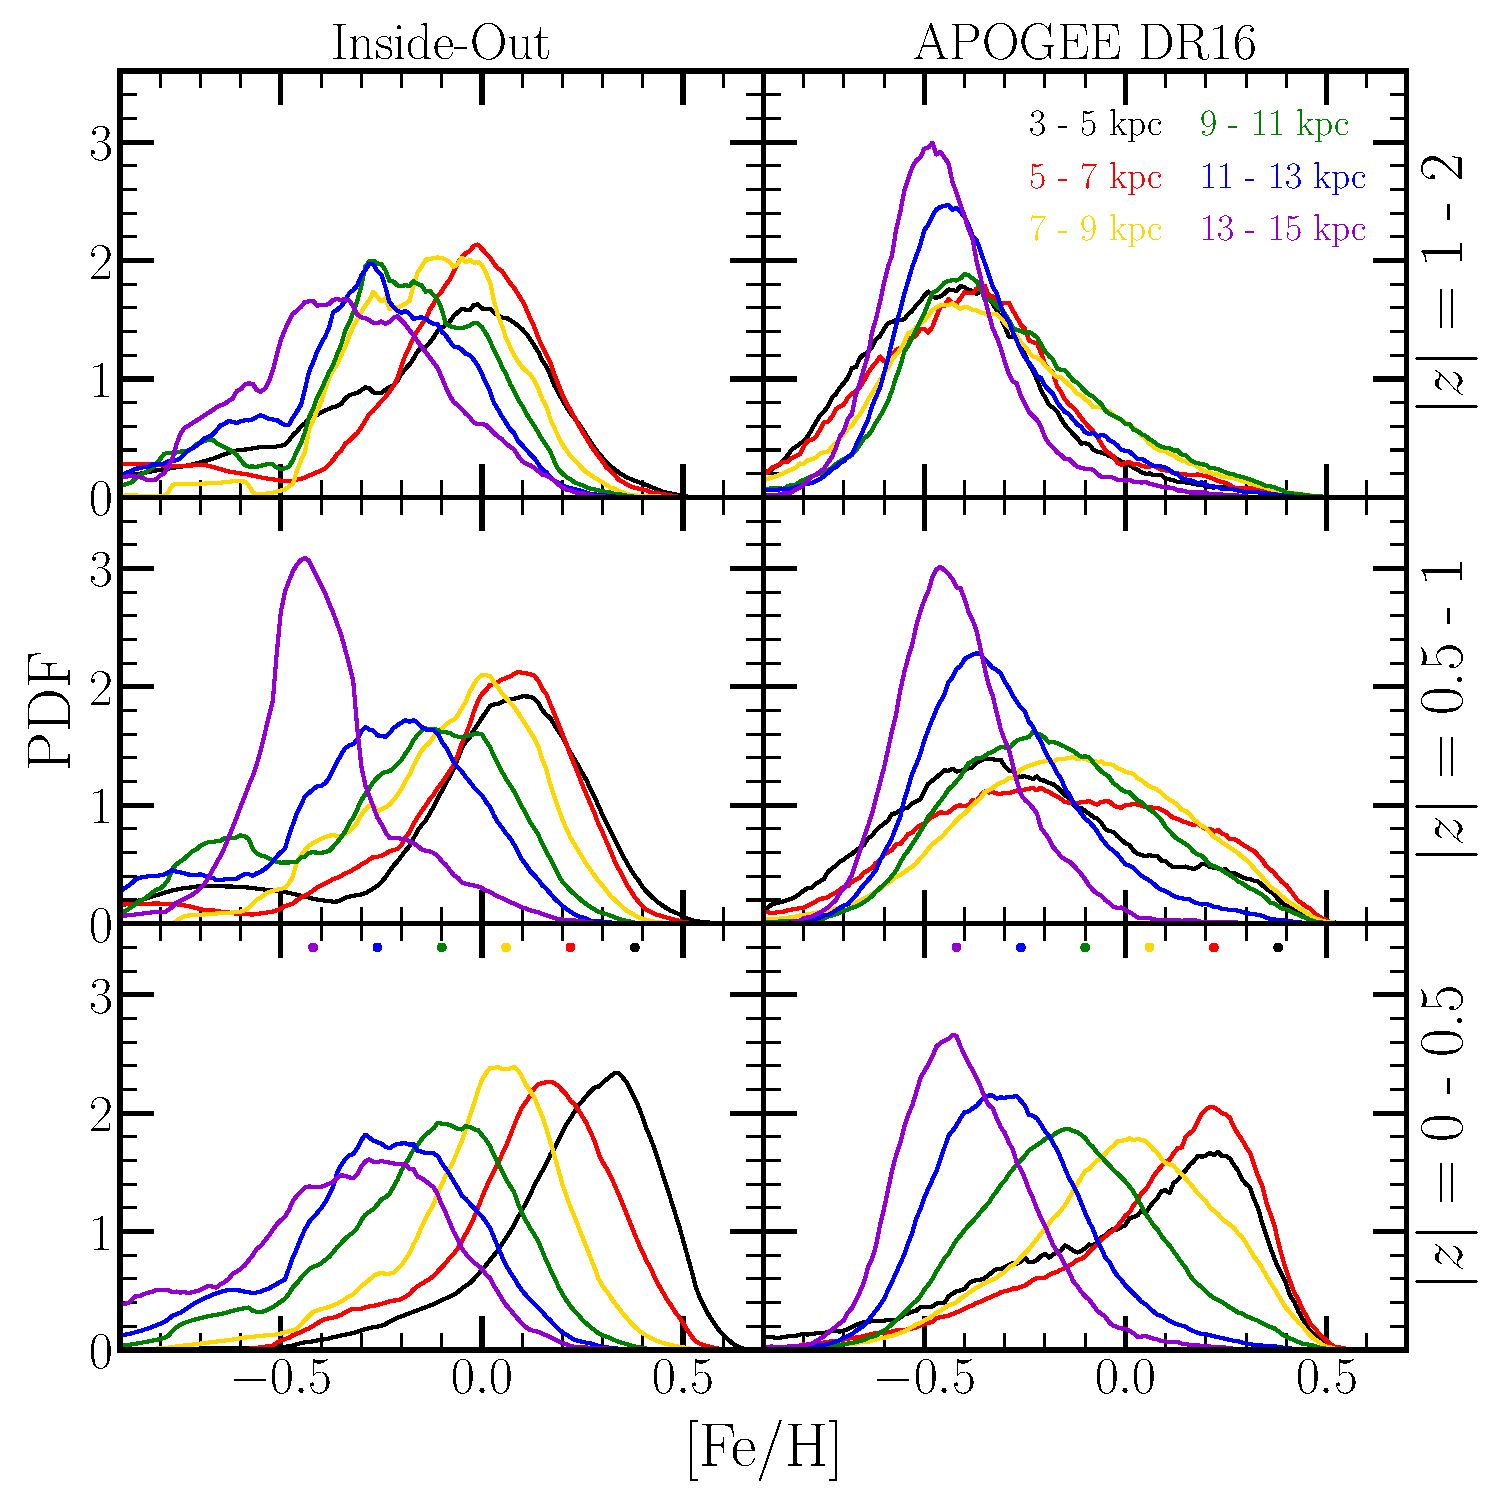
\includegraphics[scale = 0.34]{mdf_3panel_fe.pdf} 
\caption{Metallicity Distribution Functions in [Fe/H] predicted by our 
late-burst model (left) and as observed in APOGEE DR16 (right), for stars and 
simulated stellar populations with present day $\left|z\right|$ = 0 - 0.5 kpc 
(bottom), 0.5 - 1 kpc (middle), and 1 - 2 kpc (top). MDFs are shown in bins 
of Galactocentric radius: 3 - 5 kpc (black), 5 - 7 kpc (red), 7 - 9 kpc 
(yellow), 9 - 11 kpc (green), 11 - 13 kpc (blue), and 13 - 15 kpc (purple). 
The points near the top of the bottom panels denote what the mode abundance 
would be if it followed our target gradient of [Fe/H] = +0.3 at $R_\text{gal}$ 
= 4 kpc and a slope of -0.08 kpc$^{-1}$, assuming the inner radius of each bin 
(i.e. there is no point plotted for 15 kpc). All distributions are smoothed 
with a box-car width of [Fe/H]~$\pm$~0.1. } 
\label{fig:mdf_3panel_fe} 
\end{figure} 

\begin{figure} 
\centering 
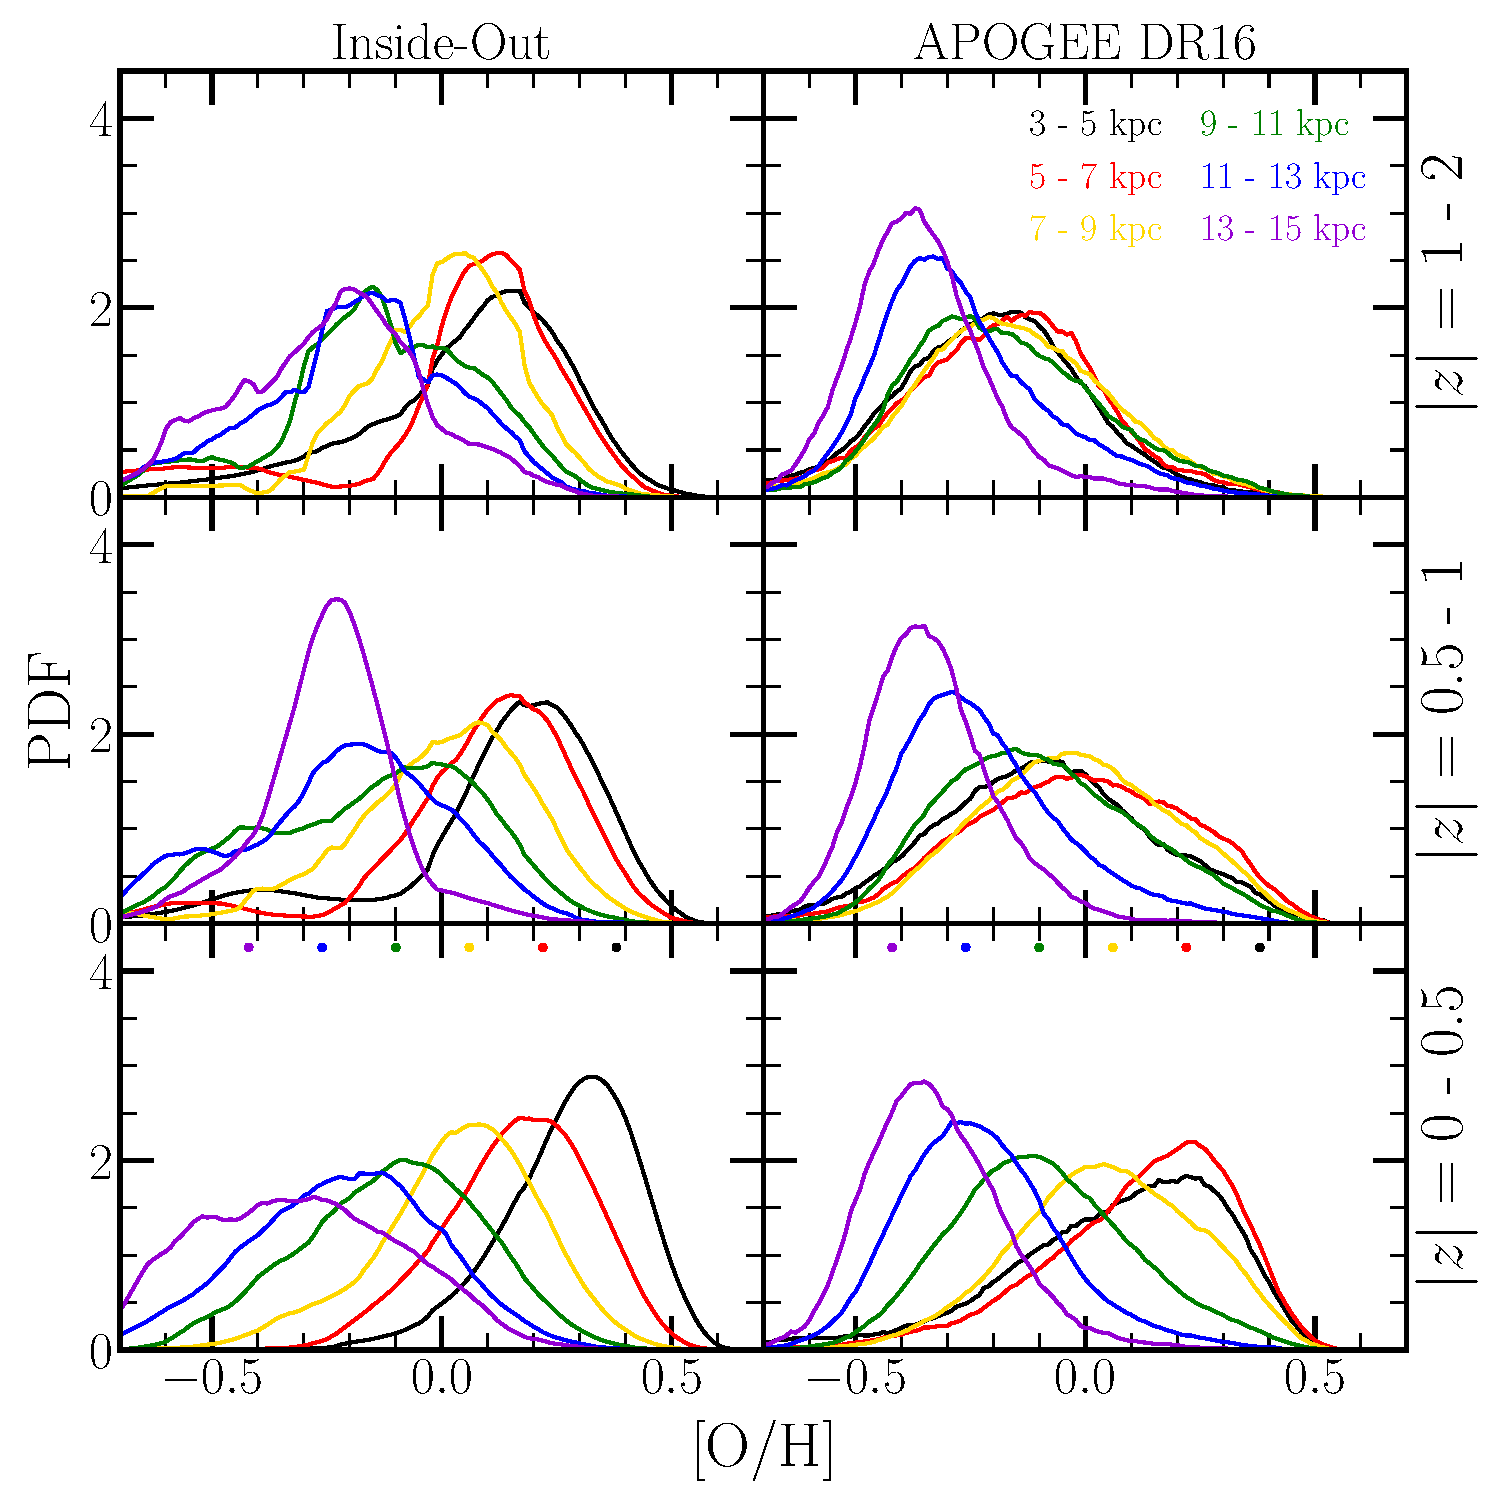
\includegraphics[scale = 0.34]{mdf_3panel_o.pdf} 
\caption{The same as Fig.~\ref{fig:mdf_3panel_fe}, but for [O/H].} 
\label{fig:mdf_3panel_o} 
\end{figure} 

\begin{figure*} 
\centering 
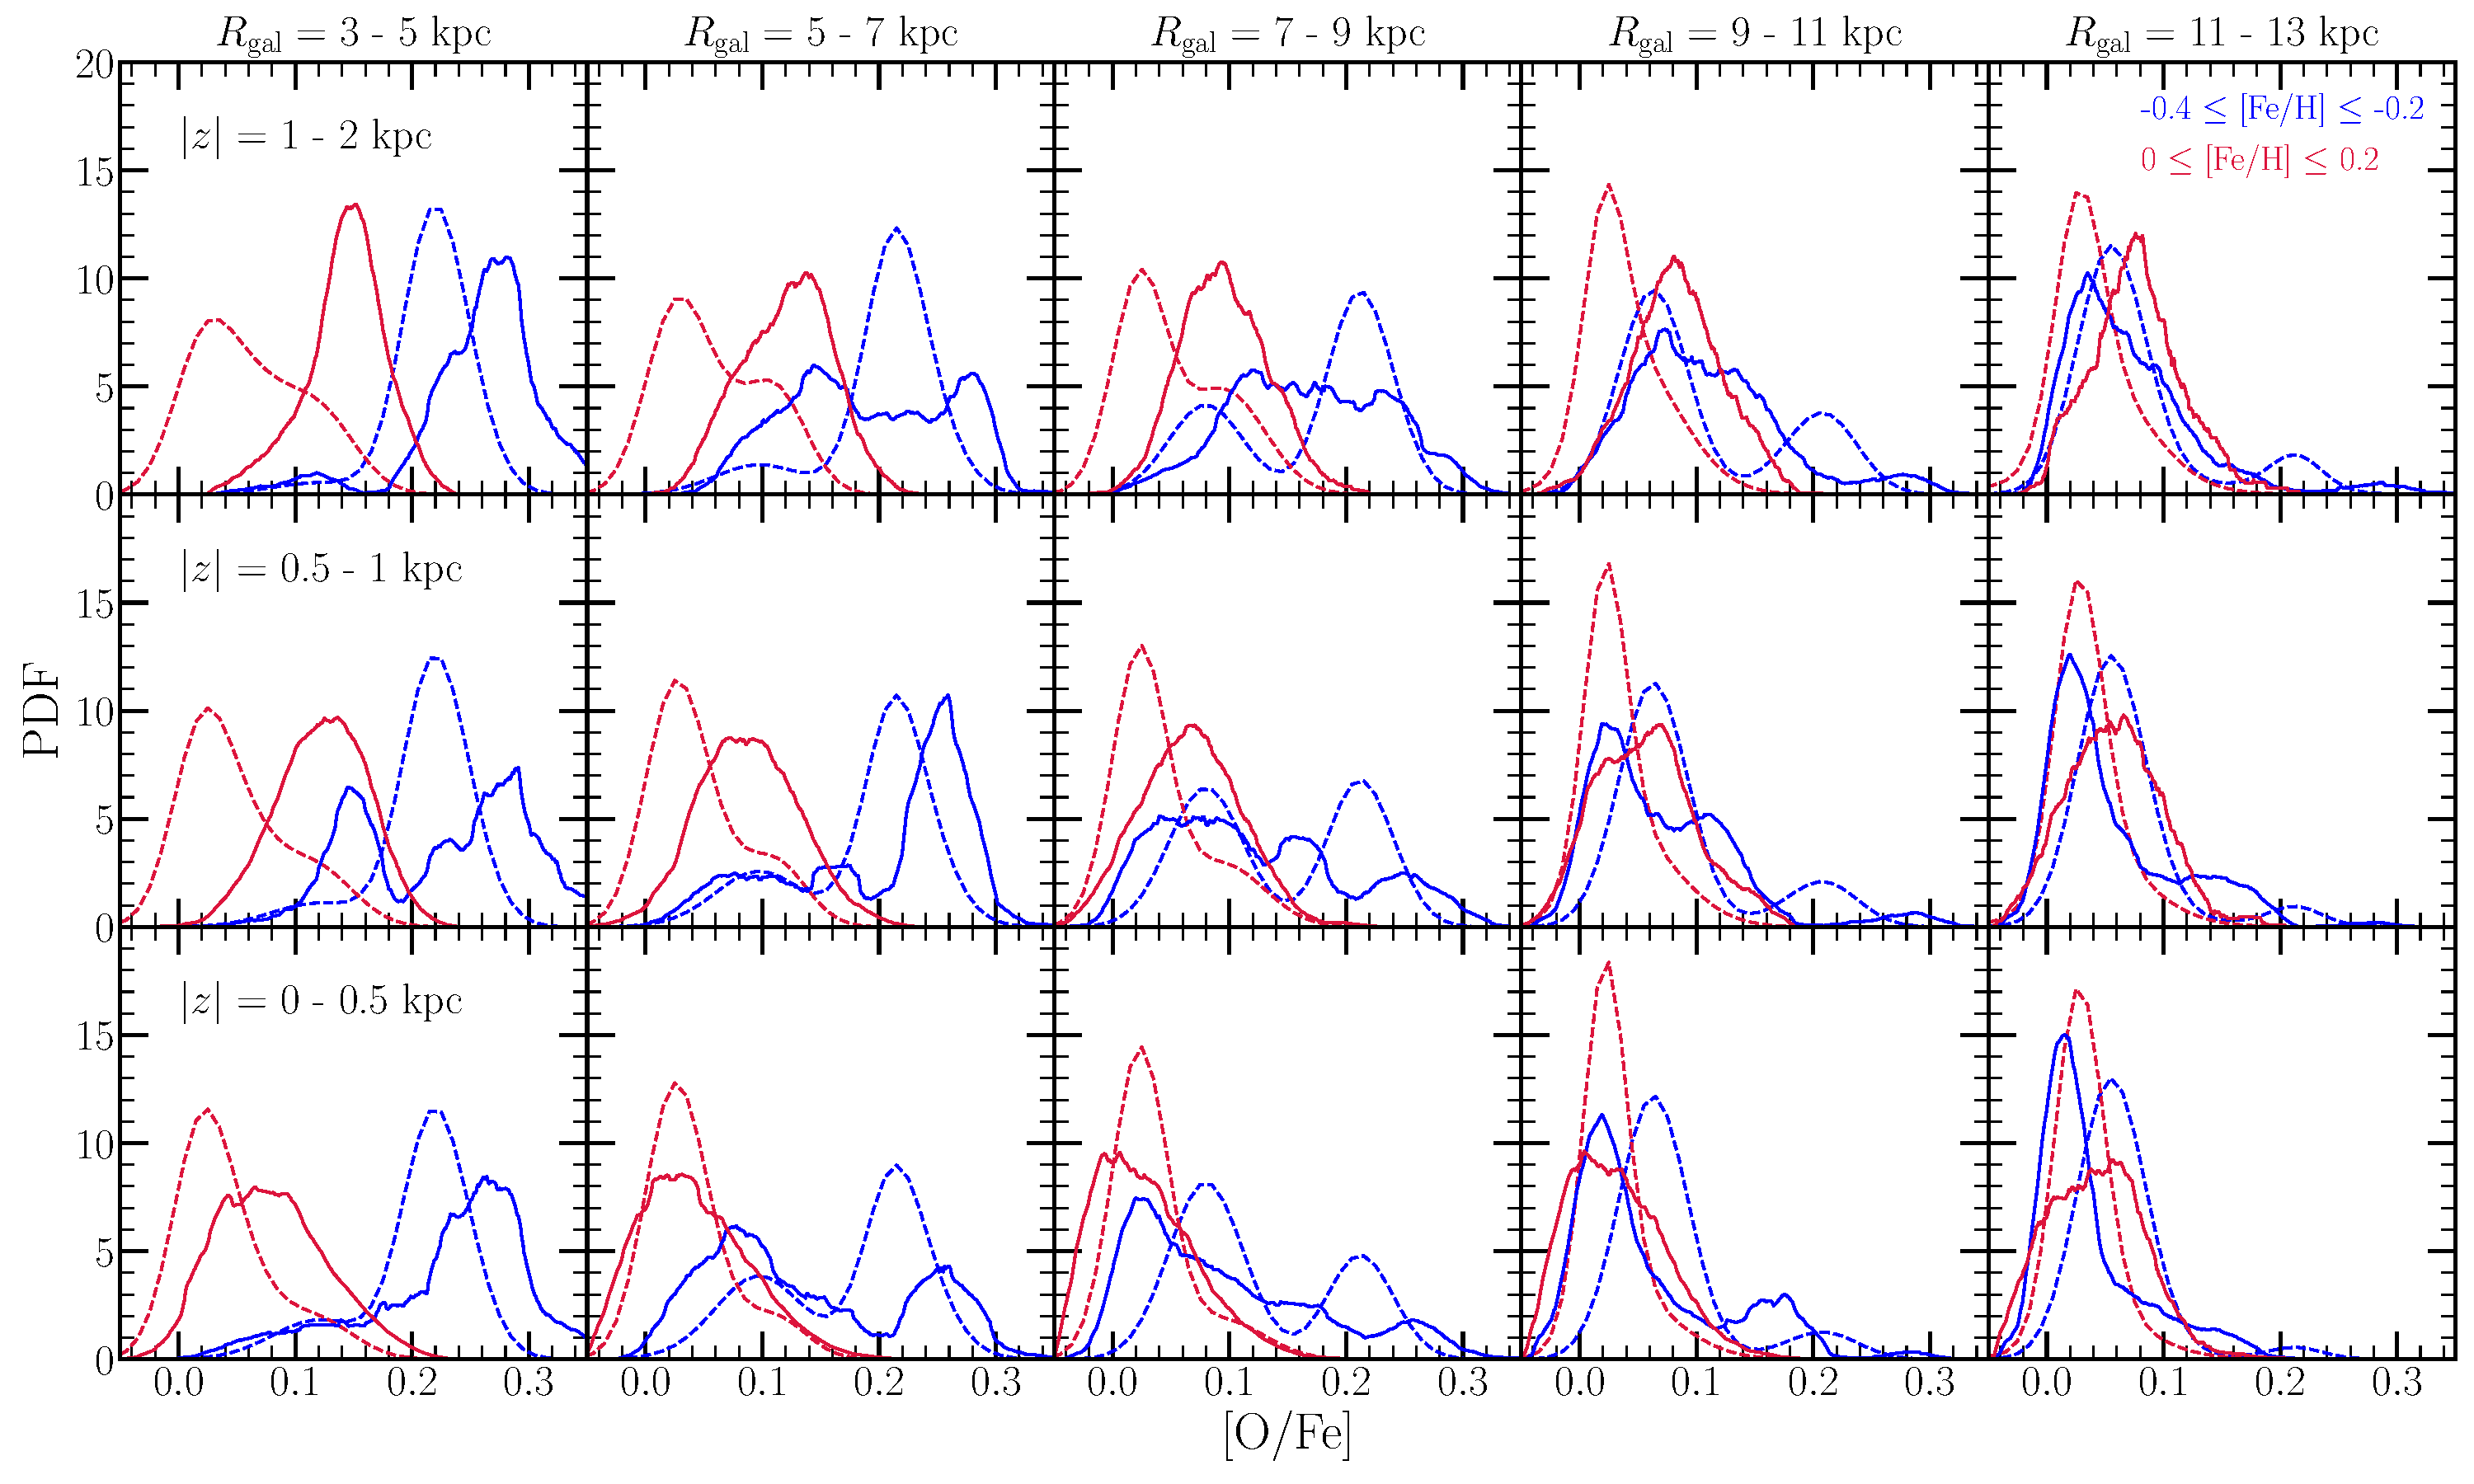
\includegraphics[scale = 0.32]{ofe_mdfs_insideout.pdf} 
\caption{Predicted distributions in [O/Fe] in 15 Galactic regions and in two 
bins in [Fe/H]. Columns correspond to bins in~$R_\text{gal}$, denoted at the 
top of each column. Rows correspond to bins in~$\left|z\right|$, denoted in 
text in the left-hand column. Distributions are color-coded according to the 
[Fe/H] the sample is drawn from, denoted by the legend in the upper right 
panel. Solid lines represent that predicted by our inside-out SFH, while 
dashed lines correspond the fits to the APOGEE DR16 data presented in Vincenzo 
et al. (2021, in prep), which quantify the intrinsic distributions accounting 
for observational uncertainties and the APOGEE selection function. Our 
simulated distributions are smoothed with a box-car width of [O/Fe]~$\pm$~0.02 
to improve clarity. }
\label{fig:ofe_mdfs_insideout} 
\end{figure*} 

\begin{itemize} 
	\item Previously known that the MDFs in the disc midplane as observed in 
	APOGEE show mode [$\alpha$/H] and [Fe/H] abundances that depend on 
	Galactocentric radius, with a skew-negative distribution in the inner 
	Galaxy and a skew-positive distribution in the outer Galaxy. Off the 
	midplane, the MDFs merge and converge on [$\alpha$/H]~$\approx$~[Fe/H] 
	$\approx$~-0.5~\citep{Hayden2015, Weinberg2019}. This result is 
	replicated for the observations in the right-hand column of panels in Fig. 
	\ref{fig:mdf_3panel_fe} and Fig.~\ref{fig:mdf_3panel_o}. 
	\begin{itemize} 
		\item Similar mode [O/H] and [Fe/H] between the 3 - 5 and 5 - 7 kpc 
		in the APOGEE observations. What could be the origin of this? 
		Cessation of star formation in the inner Galaxy? (see Fig. 1 of 
		\citealp{Peek2009} and Fig. 2 of~\citealp{Fraternali2012}). This 
		would imply very few stars formed in the most metal-rich regions of 
		the Galaxy, cutting off the MDF at high [O/H], [Fe/H]. This would 
		suggest that the Milky Way has begun the quenching of star formation, 
		a process believed to begin the centres of galaxies at this mass 
		\citep[e.g.][]{Ellison2020a}. 
	\end{itemize} 

	\item Left-hand panels of Figs.~\ref{fig:mdf_3panel_fe} 
	and~\ref{fig:mdf_3panel_o} show the distributions predicted by our 
	late-burst model. They successfully replicate the qualitative result that 
	the mode [X/H] varies with present-day Galactocentric radius, but fail to 
	show a similar mode abundance between the 3 - 5 and 5 - 7 kpc bins. 
	Potentially linked to the cessation of star formation in inner 
	Galaxy~\citep{Peek2009, Fraternali2012}, not included in our models. 

	\item Beyond the midplane, our models fail to fully replicate the 
	convergence of the MDFs at [X/H]~$\approx$~-0.5. The observed MDF at 
	small radii shifts from skew-negative with a metal-rich mode to 
	skew-positive with a metal-poor mode with increasing $\left|z\right|$. In 
	our predicted MDFs for the inner galaxy, the mode does shift to lower 
	[X/H], though not to the same extent as in the observations. There is also 
	very little change in skewness with~$\left|z\right|$ predicted, in tension 
	with observations. 
	\begin{itemize} 
		\item Could this point to a breakdown of our assumption that vertical 
		mixing is efficient? 
	\end{itemize} 

	\item We note that our models do a good job of producing a mode [X/H] 
	abundance in each radial bin close to our target gradient (shown as 
	points plotted at the top of the bottom panels in Fig. 
	\ref{fig:mdf_3panel_fe} and~\ref{fig:mdf_3panel_o} for the inner radius of 
	each 2 kpc bin). In the inner galaxy bins, the predicted mode is 
	moderately lower than the target, but this is due to the effect of 
	dilution (see discussion in~\S~\ref{sec:amr}). In our inside-out and 
	outer-burst models, the difference in target and predicted mode [X/H] is 
	considerably smaller. 
\end{itemize} 

\subsection{[O/Fe]} 
\label{sec:mdfs:ofe} 

\begin{itemize} 
	\item In this section we compare our model predicted [O/Fe] distributions 
	to those published in Vincenzo et al. (2021, in prep). These are intended 
	to simultaneously remove the effects of observational errors in [O/Fe] 
	and the APOGEE selection function in these Galactic regions; that is, 
	these are estimates of the~\textit{intrinsice} [O/Fe] distributions that, 
	when convolved with observational uncertainties and the APOGEE selection 
	function, would resemble the observed MDFs. 

	\item Fig.~\ref{fig:ofe_mdfs_insideout} show distributions in [O/Fe] in 
	two bins of [Fe/H] across 15 Galactic regions predicted by our inside-out 
	SFH (solid lines). Dashed lines show the Vincenzo et al. (2021, in prep) 
	distributions. 

	\item At fixed~$R_\text{gal}$ and [Fe/H], the Vincenzo et al. (2021, 
	in prep) MDFs show two peaks in the distribution which do not change with 
	$\left|z\right|$; only their relative heights vary. This is an assumption 
	built into the model, but the agreement with the APOGEE data is good. 
	At small~$R_\text{gal}$, the observed distributions may shift slightly to 
	higher [Mg/Fe], but only at the~$\lesssim$0.05 level between 
	$\left|z\right|\leq$~0.5 and 1~$\leq\left|z\right|\leq$~2.0 (see their Fig. 
	X). In contrast, our model predicted distributions show an increase in the 
	mode [O/Fe] of~$\sim$~0.1 over the same dynamic range in~$\left|z\right|$. 
	This suggests that our model overpredicts the increase of [O/Fe] with 
	increasing~$\left|z\right|$ compared to the APOGEE distributions. 
	{\color{red} As of now, I don't have a good explanation for why this is 
	the case. Maybe the fact that we see this at small~$R_\text{gal}$ suggests 
	the evolution of the bulge may have something to do with it? We're not 
	modeling that here.} 

	\item We note that the inside-out model fails to reproduce a Milky 
	Way-like bimodality. Such a model prediction would appear as good 
	agreement between the solid and dashed lines in Fig. 
	\ref{fig:ofe_mdfs_insideout}, but that is not the case. There may be 
	decent agreement in a given metallicity bin and Galactic region, but the 
	agreement would need to be seen everywhere and at all metallicities. 

	\item In the inner galaxy, we overestimate the [O/Fe] of the highest 
	[Fe/H] stars at all $\left|z\right|$, and the differences in the 
	distributions gets smaller with increasing~$R_\text{gal}$. The lower 
	[Fe/H] bins don't seem to have this problem. 
	\begin{itemize} 
		\item Since these are in specific bins in [Fe/H], this is an 
		indication that our model is overpredicting the O abundances of these 
		stars, rather than underpredicting [Fe/H]. 

		\item This could point to various things. Perhaps the Milky Way has 
		different gradients in [O/H] than [Fe/H], an effect which is not 
		captured by these models. Perhaps the innermost radii of the Milky 
		Way has some contamination from bulge stars, another effect which is 
		not captured by our models. Impact of bar evolution maybe? 
	\end{itemize} 

	\item Similar results are found for our other SFHs. 

	\item While the notion that an [$\alpha$/Fe] dichotomy can arise out of 
	radial migration alone was put forth in~\citet{Schoenrich2009}, and later 
	explored by~\citet{Nidever2014}, this suggests that an inside-out star 
	formation history combined with stellar migration is not conducive to 
	predicting this observed result. The principle failure of this model is 
	that it overpredicts the abundance of intermediate [$\alpha$/Fe] stars. 
	This could point to a handful of things. 
	\begin{itemize} 
		\item If the bimodality is to arise out of inside-out galaxy 
		evolution and radial migration alone, the transition between low- and 
		high-$\alpha$ sequences needs to occur faster than it does in these 
		models. Applying the analytic model of~\citet{Weinberg2017}, this can 
		be occur only with an adequately short~$\tau_\star$. Here we have 
		adopted a star formation law which is motivated by observations (see 
		discussion in~\S~\ref{sec:methods:sfe}); this suggests that the 
		observed rates of star formation are not conducive to an adequately 
		short transition between the two sequences such as to predict the 
		dichotomy in the models as it is observed in the Milky Way. 

		\item Under our current assumptions, the simplest way to achieve this 
		is to simply shut off star formation during the intermediate 
		[$\alpha$/Fe] phase in the simulations. This is indicative that 
		two-infall evolutionary histories~\citep[e.g.][]{Chiappini1997, 
		Chiappini2001, Romano2010, Grisoni2017, Noguchi2018, Spitoni2016, 
		Spitoni2018, Spitoni2019, Spitoni2020} would improve the 
		agreement between our model predictions and the observed 
		distributions. 

		\item Alternatively, there is observational evidence for a SN Ia Fe 
		yield which scales inversely with metallicity (see discussion of 
		\citealp{Brown2019} in~\S~\ref{sec:methods:yields}). If this is the 
		case, the decrease in [O/Fe] ratios at low [Fe/H] at the onset of 
		the first SN Ia events may occur faster than in our models. This may 
		predict the observed bimodality by ensuring that the transition 
		between high- and low-$\alpha$ sequences is naturally fast due to 
		supernova rates. 
	\end{itemize} 

	\item This is at 
	odds with the findings of~\citet{Sharma2020}, who claim to reproduce the 
	[$\alpha$/Fe] dichotomy with an analytic chemical evolution model with 
	an inside-out SFH and stellar migration. 
	\begin{itemize} 
		\item {\color{red} We'll need to be careful in our final draft of the 
		paper so that our language here isn't too strong. Below I've given my 
		honest critiques of the~\citet{Sharma2020} paper. } 

		\item They assume parameterized forms for [Fe/H] and [$\alpha$/Fe] as 
		functions of radius and time, chosen deliberately so 
		that they agree with the observed data. Based on dynamical arguments 
		similar to those in~\citet{Schoenrich2009}, their migration model has 
		free parameters which then require fitting to observed data. Since the 
		observed data is known to exhibit the dichotomy, their model's 
		reproduction of the observed dichotomy is not a prediction but rather 
		an assumption characterized a priori. For this reason, rather than 
		learning about the physical origins of the [$\alpha$/Fe] dichotomy 
		from~\citet{Sharma2020}, we instead get a robust mathematical 
		characterization of the data. 

		\item They find a dichotomy in the [$\alpha$/Fe]-[Fe/H] plane to 
		arise out of a fast transition in the gas phase between high-$\alpha$ 
		and low-$\alpha$. As we discussed here, we find in practice that this 
		is only the case if~$\tau_\star$ is sufficiently short, and our 
		observationally motivated scaling would suggest that the required 
		values are unphysically short ($\lesssim$1 Gyr; we find that our 
		$\tau_{\star,0}$ = 1 Gyr model also fails to reproduce an adequaately 
		fast transition). 

		\item We therefore argue that the claim of~\citet{Sharma2020} that 
		the observed dichotomy can arise purely out of inside-out galaxy 
		formation with radial migration is likely contingent upon SN Ia rates 
		scaling inversely with metallicity, as suggested by the findings of 
		\citet{Brown2019}. Under the parameters of our inside-out SFH model, 
		this is the only physically realistic means with which the predicted 
		transition between high- and low-$\alpha$ is adequately fast. 
	\end{itemize} 

	\item These findings suggest that an inside-out SFH combined with radial 
	migration, even when a late starburst is taken into account (as motivated 
	by the findings of~\citealp{Isern2019} and~\citealp{Mor2019}), 
	is~\textit{not} conducive to producing the observed [$\alpha$/Fe] 
	dichotomy. This suggests that more dramatic evolutionary events are 
	likely responsible, such as a two-infall model 
	\citep[e.g.][]{Chiappini1997, Chiappini2001, Romano2010, Grisoni2017, 
	Noguchi2018, Spitoni2016, Spitoni2018, Spitoni2019, Spitoni2020}. 
\end{itemize} 


\section{The Age-[$\alpha$/Fe] Relation} 
\label{sec:age_alpha} 

\begin{figure*} 
\centering 
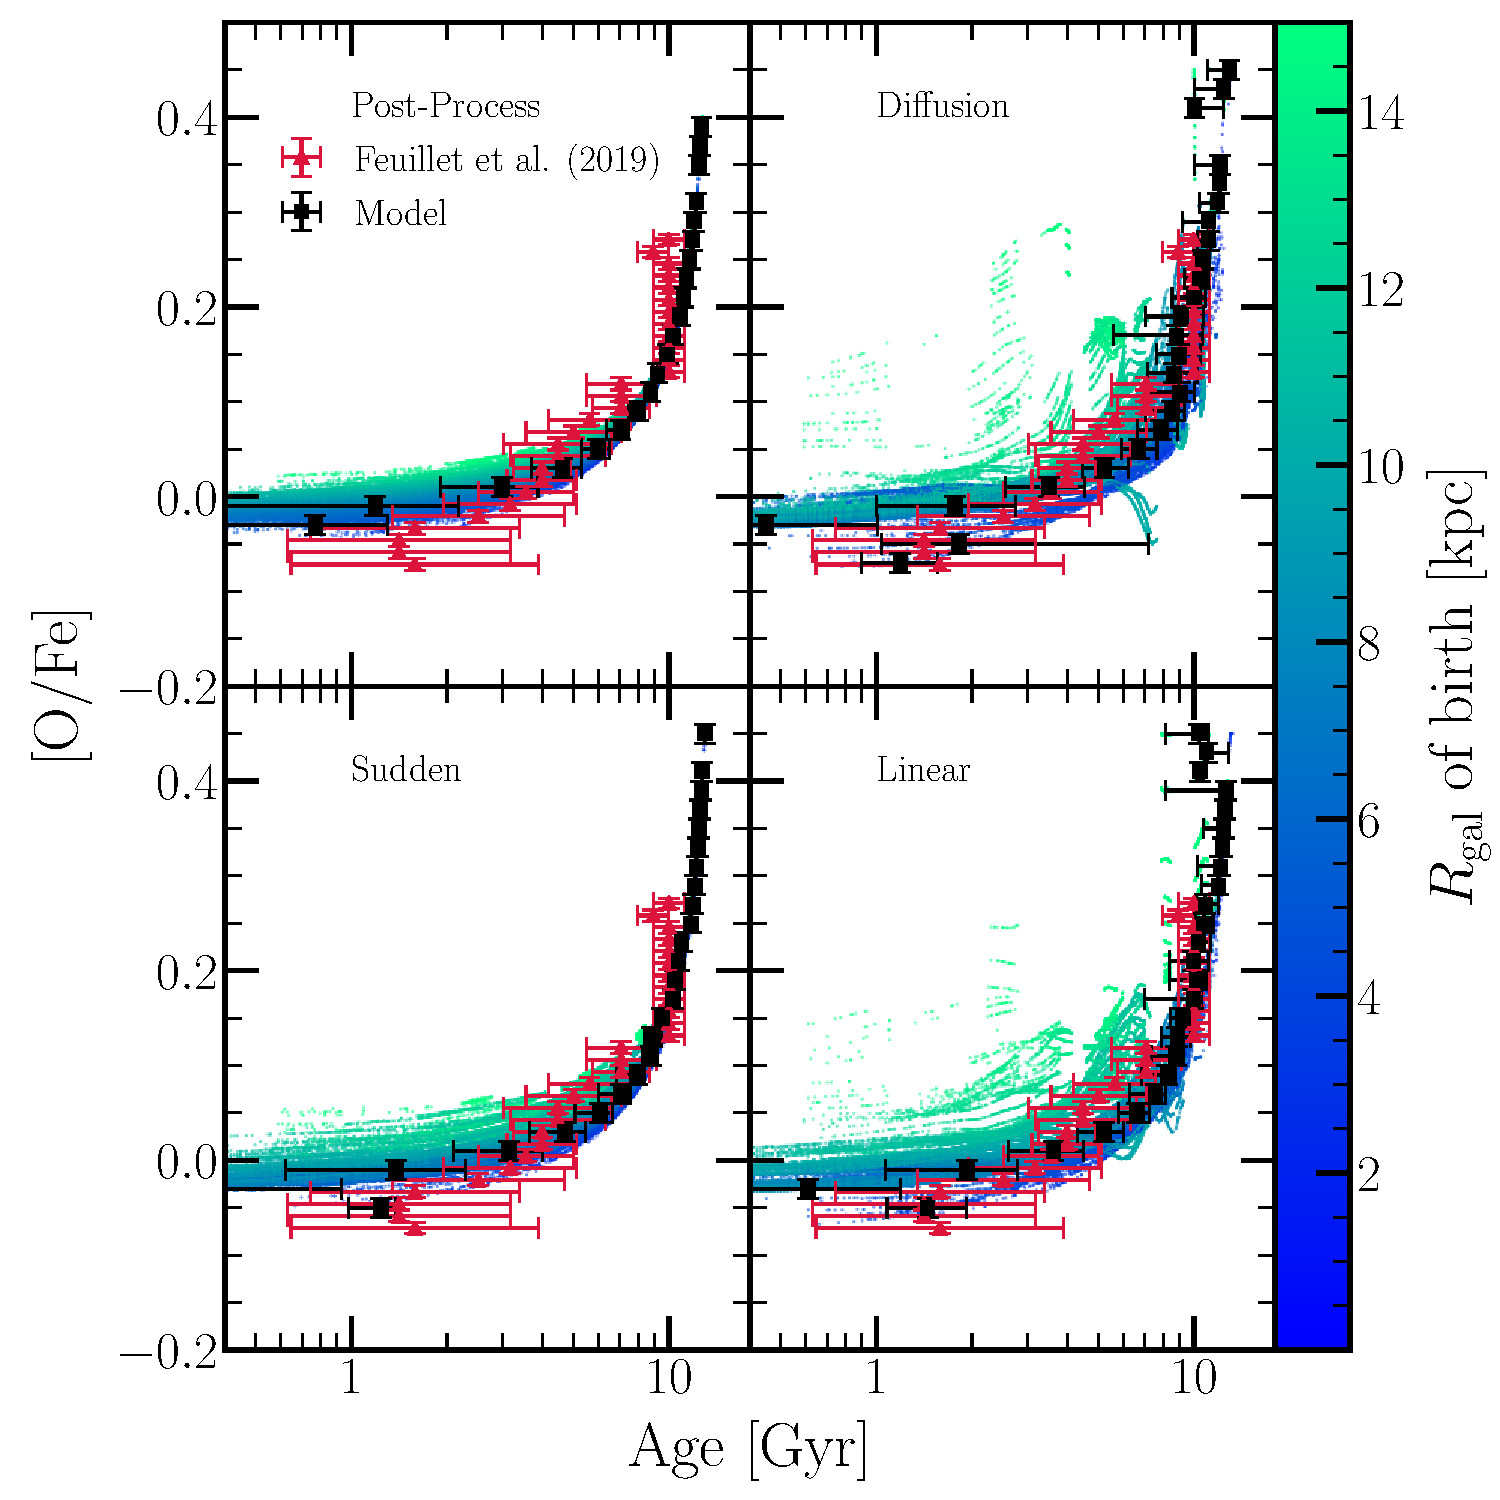
\includegraphics[scale = 0.34]{age_ofe_migration_comparison.pdf} 
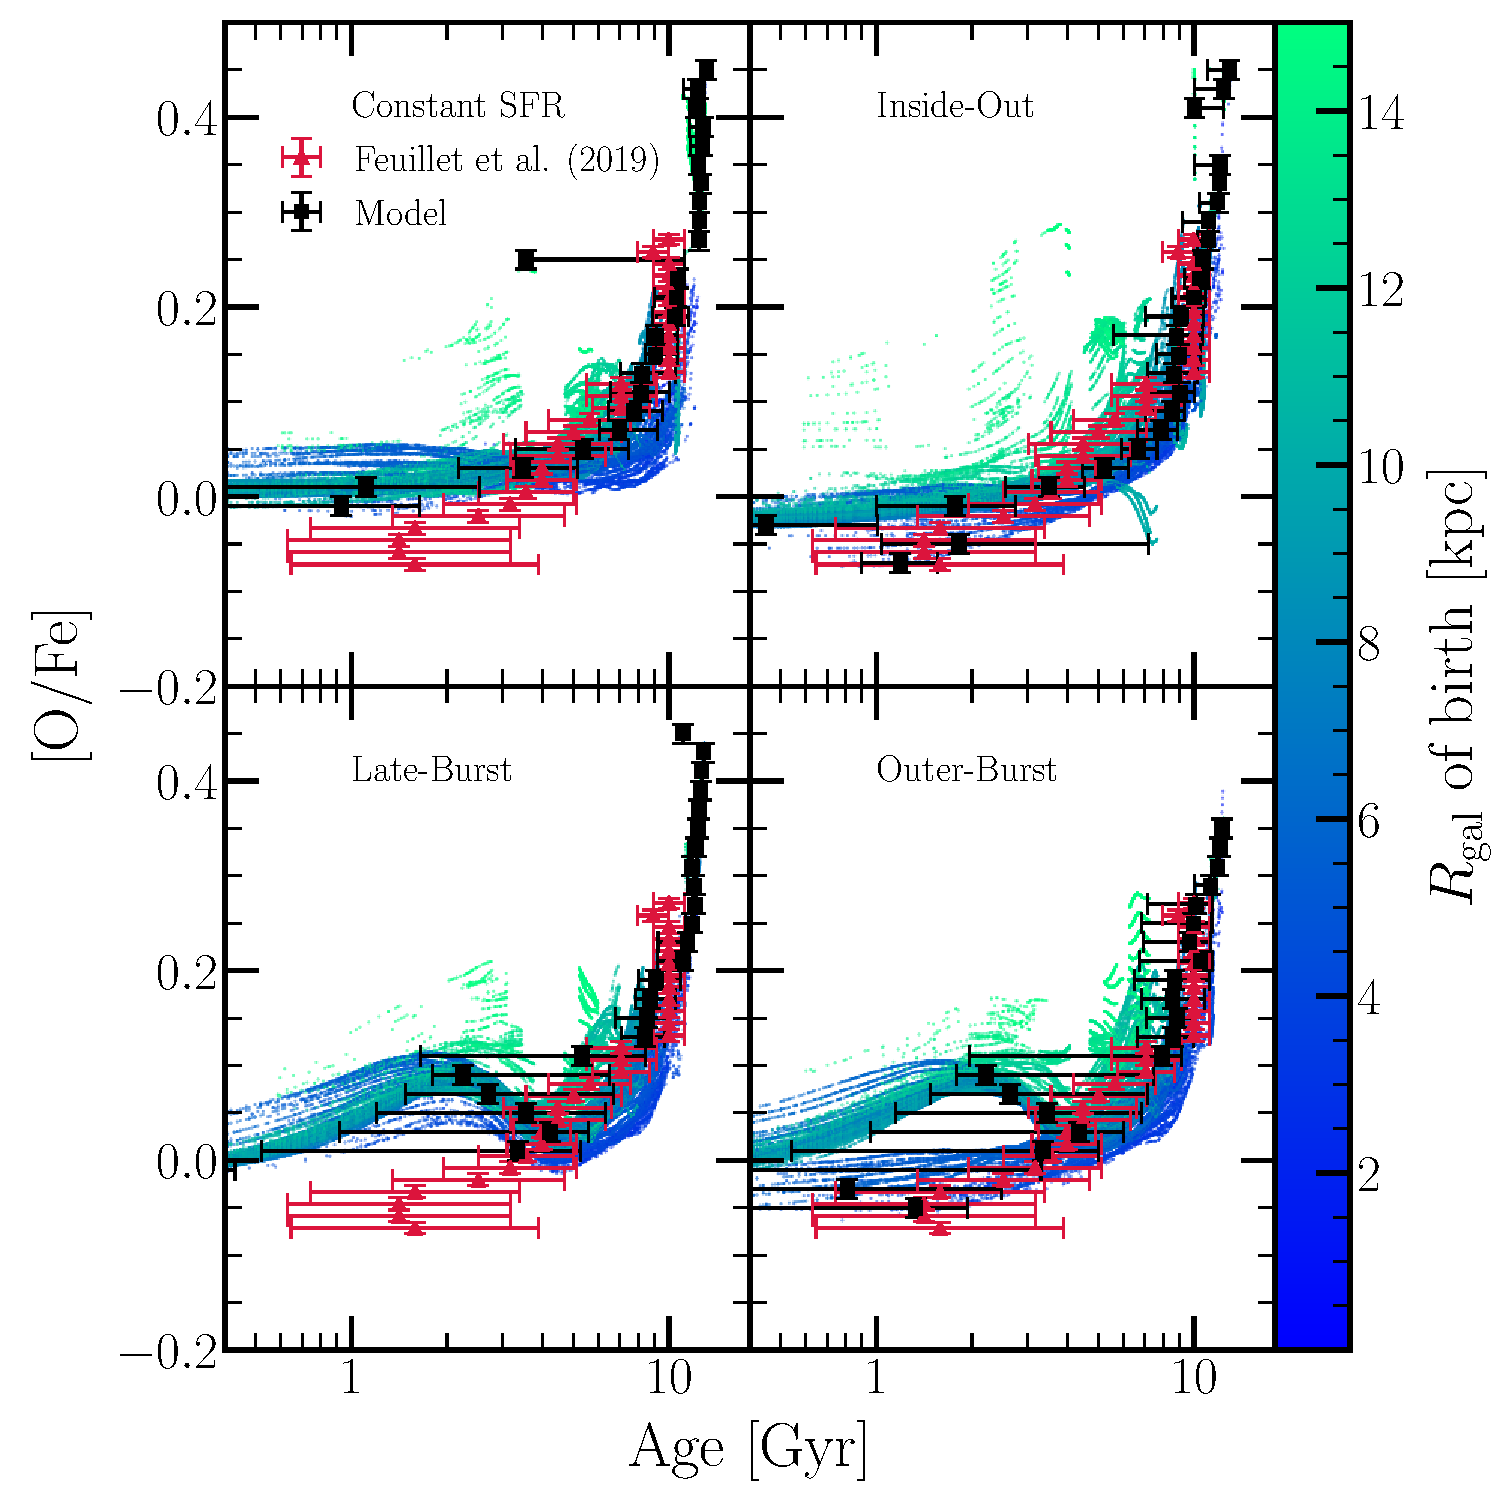
\includegraphics[scale = 0.34]{age_ofe_sfh_comparison.pdf} 
\caption{
\textbf{Left}: A comparison of the predicted age-[O/Fe] relation for the 
solar annulus ($R_\text{gal}$ = 7 - 9 kpc and $\left|z\right|\leq$ 0.5 kpc) 
between the post-processing (upper left), diffusion (upper right), sudden 
(lower left), and linear (lower right) migration models, assuming our 
inside-out SFH. 
\textbf{Right}: The same as the left-hand panels, instead comparing the impact 
of our constant (upper left), inside-out (upper right), late-burst (lower 
left), and outer-burst (lower-right) SFHs. 
In all panels, red triangles and error bars denote the observed mean age and 
dispersion thereof in bins of [O/Fe] as reported by~\citet{Feuillet2019}; here 
we include only the bins containing at least 15 stars. Black squares denote 
the mass-weighted median age in 0.02-dex bins in [O/Fe] predicted by the 
simulations, with error bras denoting the 16th and 84th percentiles of the 
mass-weighted age distribution in those bins. Points in the background denote 
each individual stellar population from the simulation with a final position 
in the solar annulus, color-coded according to their Galactocentric radius of 
birth. 
} 
\label{fig:age_alpha} 
\end{figure*} 

\begin{figure*} 
\centering 
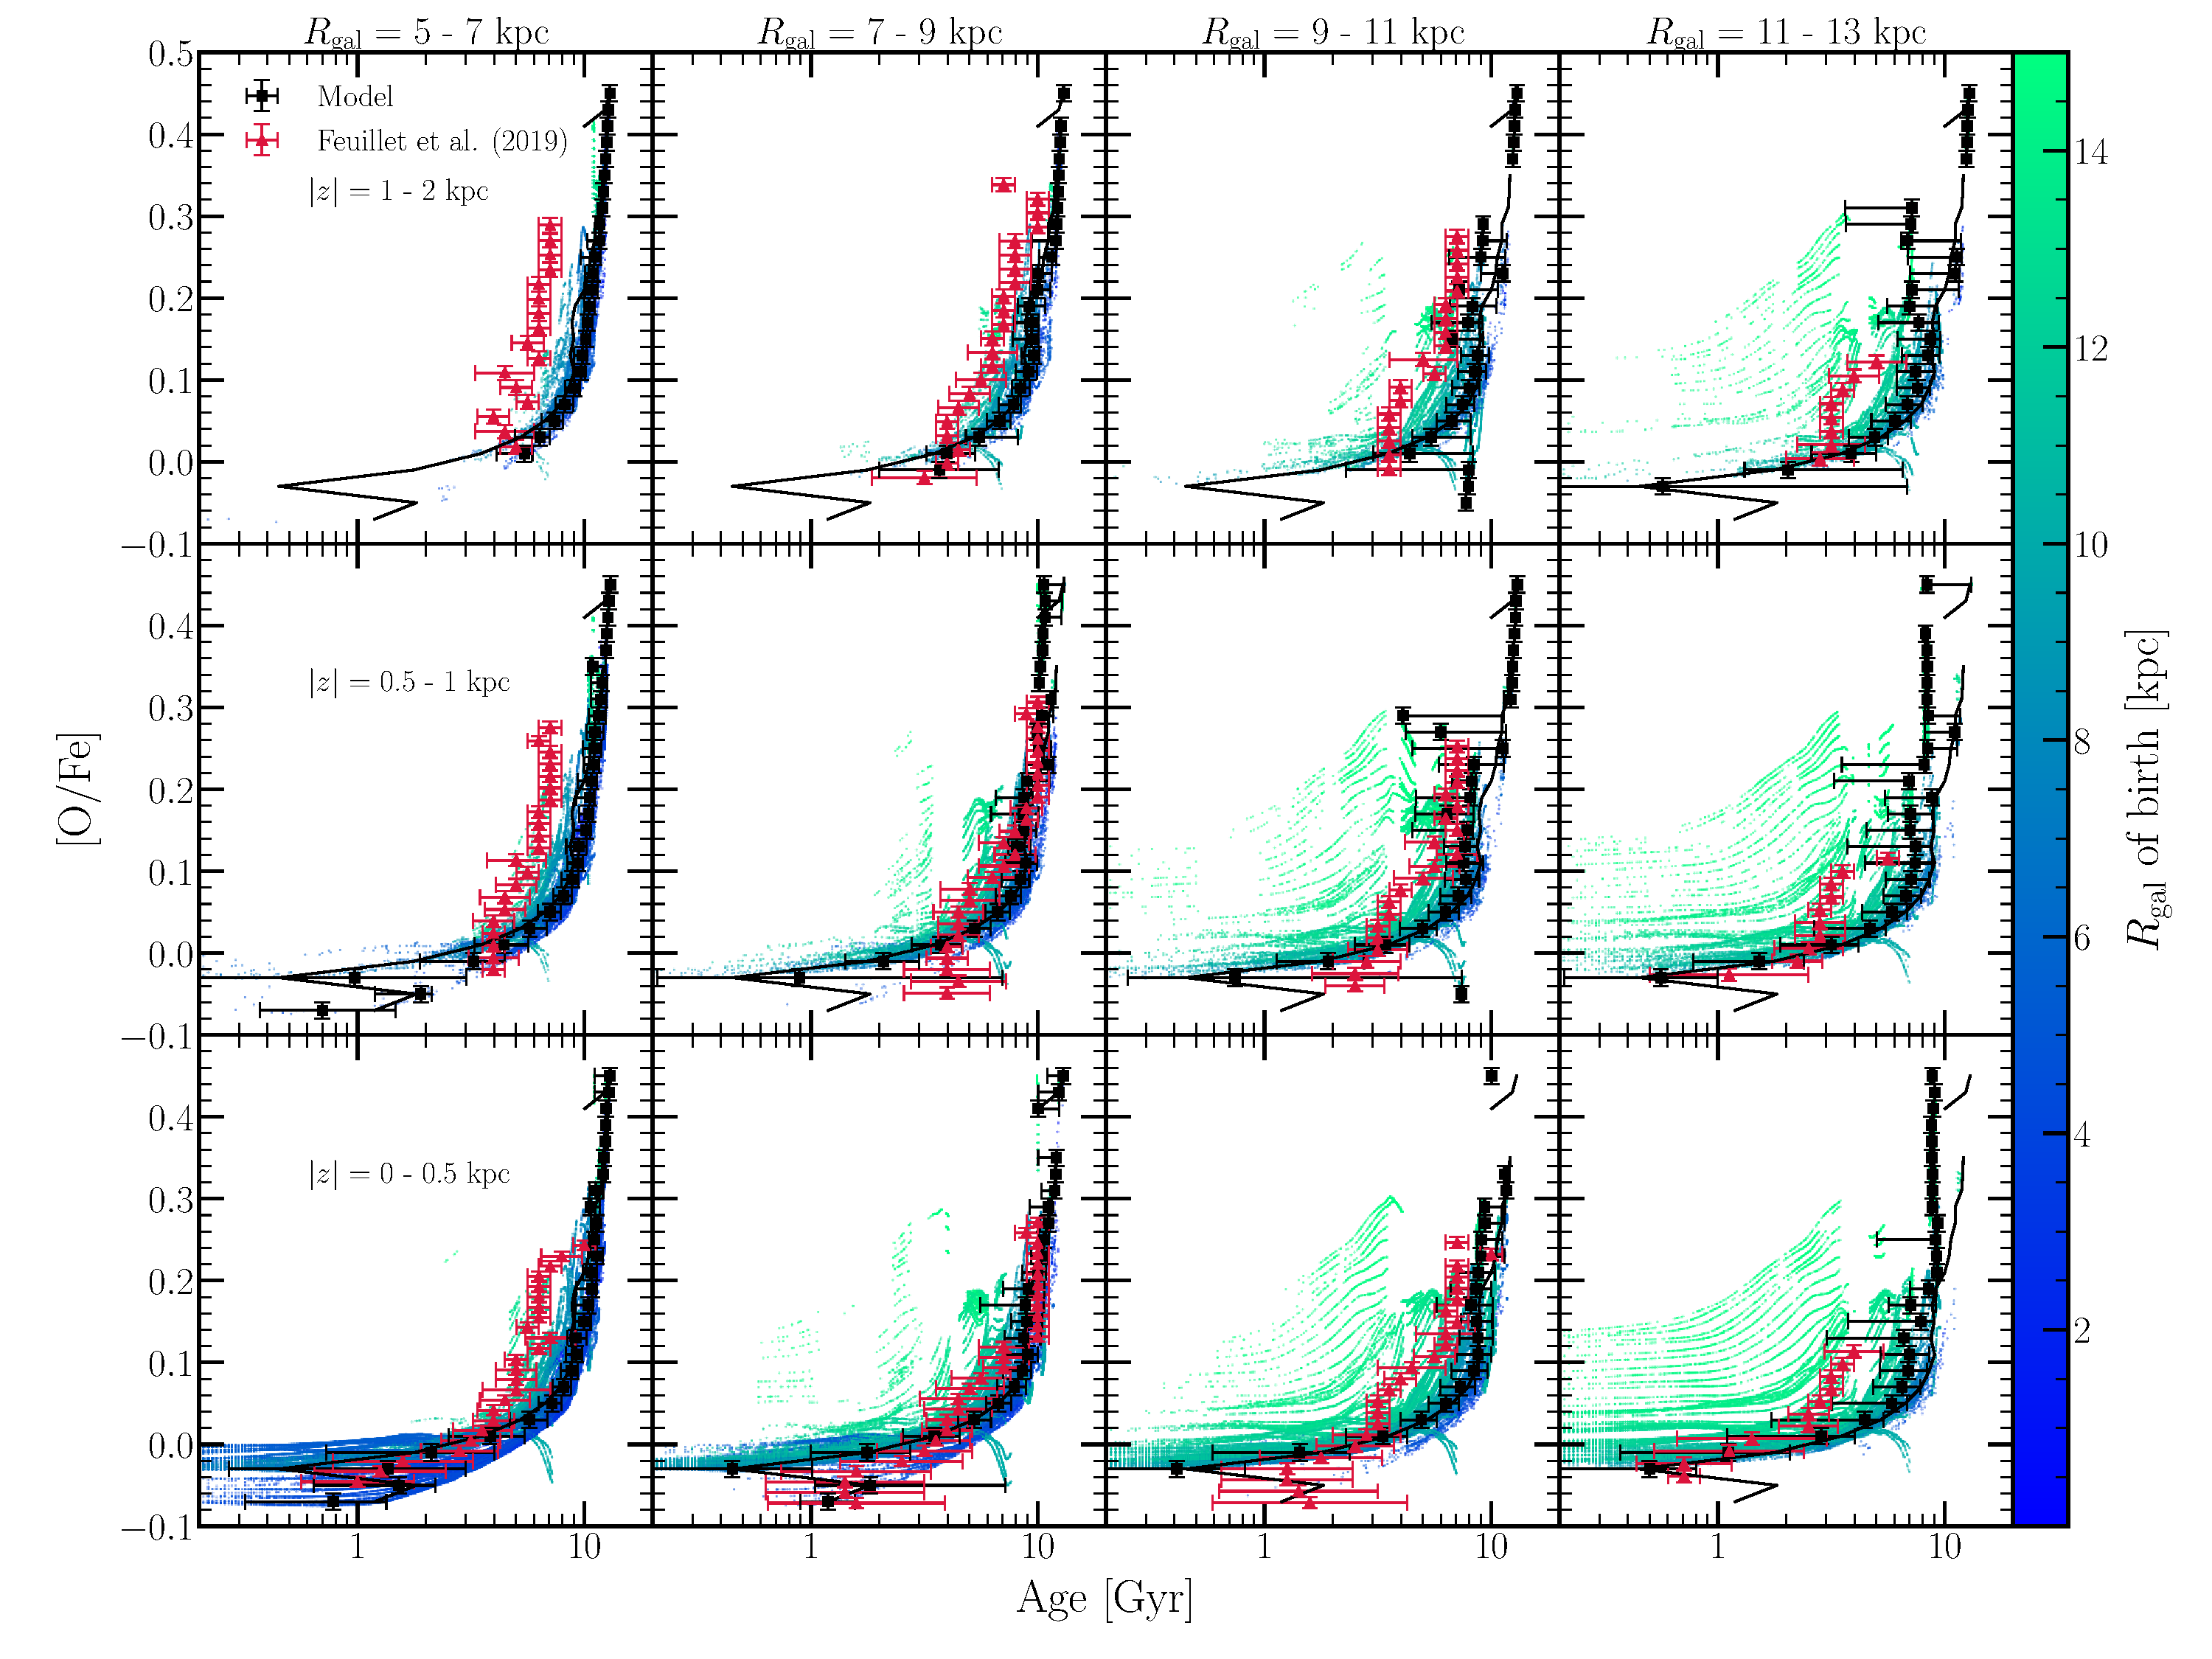
\includegraphics[scale = 0.32]{age_alpha_regions.pdf} 
\caption{The age-[O/Fe] relation in 12 galactic regions predicted by 
our inside-out SFH. Bins in Galactocentric radius are shown in columns, 
and labeled at the top. Bins in the height $\left|z\right|$ above/below the 
disc midplane are shown in rows, noted in the left-hand column. Red triangles, 
black squares, error bars, and background points are as in 
Fig.~\ref{fig:age_alpha} for the corresponding Galactic 
region. 
} 
\label{fig:age_alpha_regions} 
\end{figure*} 

\begin{itemize} 
	\item In this section, we compare our model predictions to the 
	observational results of~\citet{Feuillet2019}. While we made use of 
	APOGEE DR16 data in comparing our model predictions to the observed 
	MDFs~\citep{Ahumada2020, Majewski2017}, they make use of DR14 stars which 
	have Gaia parallax measurements available~\citep[][for details on the 
	APOGEE survey, see discussion in~\S~\ref{sec:mdfs}]{Abolfathi2014, 
	GaiaDR2}. With their spatial and quality cuts, the final sample consisted 
	of 77,562 stars. 

	\item \citet{Feuillet2019} ages are measured via isochrone matching. 
	{\color{red} Potentially give a little more detail, but that may be 
	adequate for our purposes.} 

	\item In bins of [O/Fe], they assume a gaussian age distribution, and fit 
	the mean and standard deviation to the observed sample. Because they 
	assume a gaussian, they would report an equal mean and median. This is an 
	important caveat in comparing our predicted relations to their results, 
	because our model-predicted age distributions in bins of abundace are 
	highly non-gaussian. 

	\item The stellar populations from our simulations have different masses, 
	so the age-distributions must be weighted by mass, since that scales with 
	the number of stars that each stellar population represents. We therefore 
	adopt a mass-weighted median age in bins of abundance as the appropriate 
	comparison to the~\citet{Feuillet2019} data. Physically, in a given bin 
	[O/Fe], this is the age corresponding to the 50th percentile of the 
	mass-weighted age distribution of our simulated stellar populations. For 
	these reasons the comparison between our simulations and 
	\citet{Feuillet2019} isn't exactly one-to-one. {\color{red} Potentially 
	worth mentioning some of the systematics in calculating ages here as 
	well, as that's relevant information.} 
\end{itemize}

\subsection{The Impact of Radial Migration} 
\label{sec:age_alpha:migration} 
\begin{itemize} 
	\item Fig.~\ref{fig:age_alpha} shows a comparison 
	between the predicted age-[$\alpha$/Fe] relations in the solar annulus for 
	our four migration models assuming our inside-out SFH. 

	\item All models show reasonable agreement with the~\citet{Feuillet2019} 
	data; the population-averaged trend appears insensitive to the assumed 
	migration model. 

	\item Diffusion predicts the most intrinsic scatter, followed by linear, 
	then sudden, then post-processing. This is a consequence of the variations 
	in the SN Ia rates induced by time-dependent migration (see discussion in 
	\S~\ref{sec:metallicity_space}). Further demonstration that under 
	certain migration models, the radial migration of nucleosynthetic yields 
	is statistically significant. This is also proof of concept that the 
	effect is significant for abundance ratios of elements where at least one 
	is produced by delayed nucleosynthetic sources. We therefore conclude that 
	the time-dependence of radial migration is a necessary ingredient to 
	chemical evolution models of galaxies where migration plays an important 
	role, such as our own Milky Way. The level of scatter also appears to 
	depend noticeably on which model for the time-dependence is adopted. 

	\item This mechanism can produce populations of Fe-poor or Fe-rich stars, 
	which can be misinterpreted as $\alpha$-enhanced or $\alpha$-deficient 
	stars. Due to young stars migrating into or out of a given annulus, the SN 
	Ia rate may be higher or lower than the expectation from a post-processing 
	migration model. If this difference in the SN Ia rate is sustained for of 
	order one depletion time, the ISM will be either Fe-poor or Fe-rich, and 
	the stars that form there will inherit that composition.\footnote{
		{\color{red} Potentially note the~\citet{Weinberg2017} definition: 
		$\tau_\text{dep} \equiv \tau_\star/(1 + \eta - r)$. Even with 
		$\tau_\star$ as high as~$\sim$5 Gyr at large Galactocentric radii, 
		depletion times are still short due to the high values of $\eta$ 
		there.}
	} The stars that form out of that patch of ISM can then migrate to the 
	solar annulus. This effect is most significant at large Galactocentric 
	radii where the fractional amplitude of the variability in the SN Ia rate 
	is largest, and for that reason the young Fe-poor population predicted by 
	our diffusion model originates at large radii ($\gtrsim$ 12 kpc). 

	\item \citet{SilvaAguirre2018} demonstrated that the observed young 
	$\alpha$-rich stars in the solar annulus have kinematics similar to the 
	rest of the high-$\alpha$ population, and suggested that this may be the 
	result of stellar mergers or mass transfer events, producing a population 
	of truly old stars masquerading as young stars. This would imply that the 
	observed young $\alpha$-rich population is actually just older, 
	high-$\alpha$ stars that have gone through some special class of stellar 
	evolution. Our model predicts intrinsically young, Fe-poor stars to 
	explain the observations, but these interpretations are not mutually 
	exclusive. It's possible that some of the observed stars are truly young, 
	Fe-poor stars, and that others underwent some stellar interaction event. 
	Ascertaining the origins of this population therefore has implications for 
	which of the migration models investigated here is the most realistic. 
\end{itemize} 

\subsection{The Impact of the Star Formation SFH} 
\label{sec:age_alpha:sfh} 
\begin{itemize} 
	\item Fig.~\ref{fig:age_alpha} shows a comparison between 
	the predicted age-[$\alpha$/Fe] relations in the solar annulus for our 
	four SFHs assuming diffusion migration. 

	\item Constant and inside-out SFHs describe the observed data the best. 
	Both late starburst models show a population-averaged increase in 
	[$\alpha$/Fe] at young ages which is not observed in the data. This 
	challenges the results of~\citet{Isern2019} and~\citet{Mor2019}, 
	suggesting that these results on the Milky Way recent SFH are not 
	consistent with chemical evolution models. If the Milky Way truly 
	experienced a recent starburst, something not included in our models had 
	to occur to prevent this global increase in [$\alpha$/Fe]. 

	\item Below [O/Fe]~$\approx$ +0.1, the~\citet{Feuillet2019} data seem to 
	follow a slightly steeper age-[$\alpha$/Fe] than our inside-out model 
	predicts. This likely points to inaccuracies in the detailed form of the 
	SFH or the SN Ia DTD, both of which are very plausible. 
\end{itemize} 

\subsection{Beyond the Solar Annulus} 
\label{sec:age_alpha:beyond_solar_annulus} 
\begin{itemize} 
	\item Fig.~\ref{fig:age_alpha_regions} presents a comparison of our 
	simulation data to the~\citet{Feuillet2019} observational data in 12 
	Galactic regions assuming the inside-out SFH. 

	\item In the disc, the inside-out SFH is a reasonable description of the 
	data for ages~$\lesssim$ 5 Gyr, above which the median ages are 
	overpredicted relative to~\citet{Feuillet2019}. Far from the midplane, our 
	model overpredicts the ages at nearly all abundances 
	where~\citet{Feuillet2019} have data, with the exception of the 
	$R_\text{gal}$ = 7 - 9 kpc and $\left|z\right|$ = 0.5 - 1 kpc region. 

	\item Differences in ages are interesting though - nearly everywhere we 
	overpredict ages relative to~\citet{Feuillet2019}, their data are 
	reasonably described by the stellar populations from our simulations that 
	we would classify as Fe-poor (see discussion in~\S 
	\ref{sec:age_alpha:migration}). Especially noticeable in the
	$R_\text{gal}$ = 5 - 7 kpc, where the observed sample agrees nearly 
	perfectly with one particular Fe-poor population in the 
	$\left|z\right|\leq$~0.5 kpc and 0.5~$\leq\left|z\right|\leq$~1.0 kpc 
	regions. In the~$\left|z\right|\leq$ 0.5 kpc population, the observed 
	data even show an abrupt increase in age near the maximum [O/Fe] ratio of 
	this particular subset of our stellar populations, and have one data point 
	that agrees with the population-averaged trend in our simulation. 
	\begin{itemize} 
		\item Taking the~\citet{Feuillet2019} data at face value, this would 
		suggest that our simulation is overpredicting the rate of Fe injection 
		from SN Ia, implying a SN Ia DTD whose characteristic timescales are 
		longer than we employ here, thus slowing the decrease of [$\alpha$/Fe] 
		with time. 

		\item Taking the simulation results at face value, this would suggest 
		that APOGEE+Gaia target selection favors the stars we would classify 
		as Fe-poor. 

		\item This is another instance where a two-infall model would help 
		improve the fit, however~\citep[e.g.][]{Chiappini1997, Chiappini2001, 
		Romano2010, Grisoni2017, Noguchi2018, Spitoni2016, Spitoni2018, 
		Spitoni2019, Spitoni2020}. Through a perturbation of 
		the ratio of CCSN to SN Ia rates~\citep[e.g.][]{Johnson2020}, the 
		model would predict an increase in [$\alpha$/Fe] at ages of 
		$\sim$8 - 10 Gyr following the formation of the high-$\alpha$ 
		sequence, decreasing toward younger ages. Although this would worsen 
		the agreement in the solar annulus, it would improve it in other 
		Galactic regions. 
	\end{itemize} 

	\item We note that the intrinsic scatter in the age-[$\alpha$/Fe] relation 
	predicted by the model grows with increasing~$R_\text{gal}$. Not only is 
	the scatter in the colored background points visibly larger, but the error 
	bars on the black points are as well, indicating that the age distribution 
	is getting statistically significantly wider at fixed [$\alpha$/Fe] with 
	increasing~$R_\text{gal}$. 
	\begin{itemize} 
		\item This is due to the variability in the SN Ia rates in each of 
		our model's annuli that we described in~\S~\ref{sec:metallicity_space}. 
		There, we demonstrated that the highest amplitude variability in the 
		SN Ia rate in our model galaxy is in the outskirts of the disc. This 
		arises out of time-dependent migration inducing a variability; this 
		variability gets larger in our models in regions where the stellar 
		number density is low. 

		\item With a higher variability in the SN Ia rate comes a higher 
		variability in the rate of Fe production. Therefore, stars at large 
		$R_\text{gal}$ form out of an ISM with an [O/Fe] ratio that is more 
		variable, the observational signature of which is the intrinsic 
		scatter in the age-[$\alpha$/Fe] relation growing with~$R_\text{gal}$. 
	\end{itemize} 
\end{itemize} 

\section{The Age-Metallicity Relation} 
\label{sec:amr} 

\begin{figure} 
\centering 
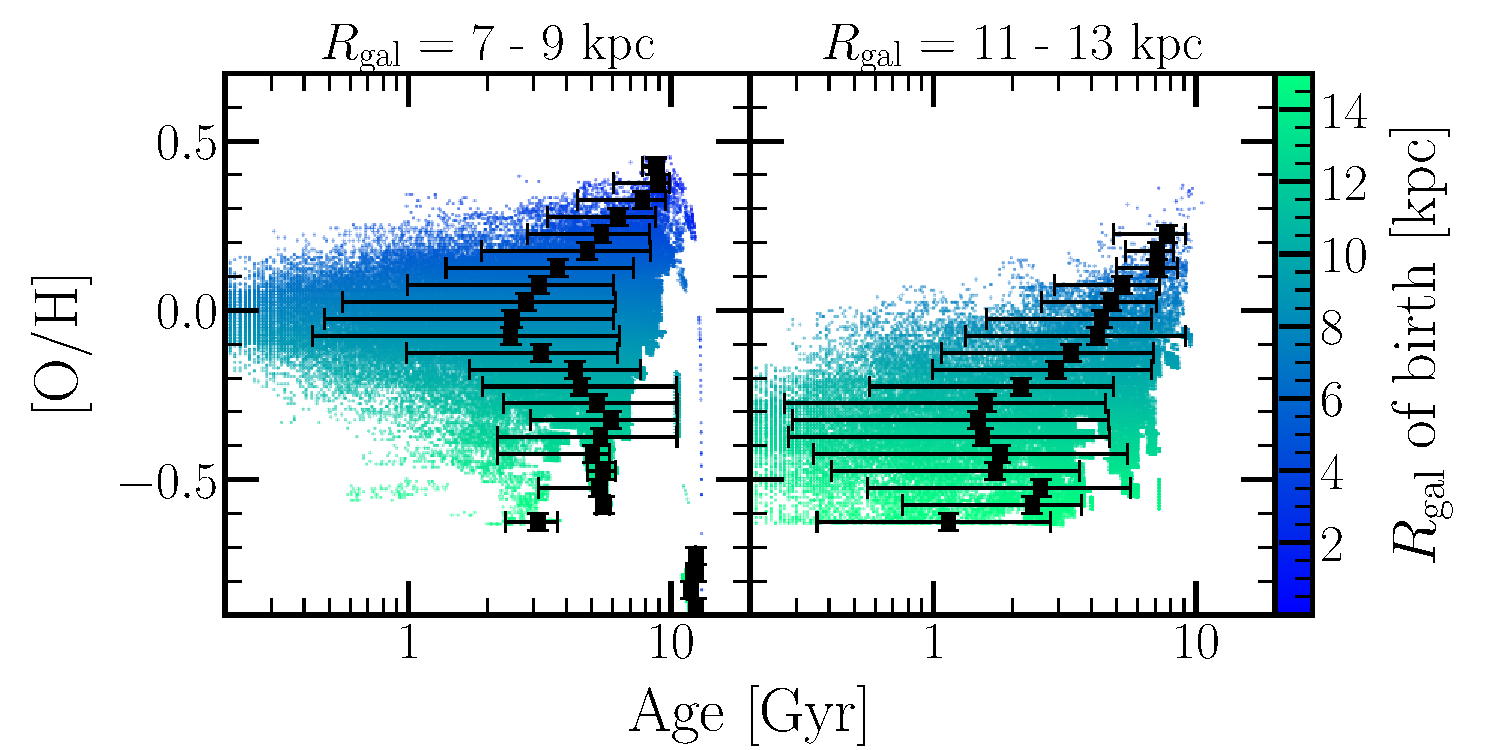
\includegraphics[scale = 0.35]{amr_static_o.pdf} 
\caption{The age-[O/H] relation predicted by our constant SFR model for 
$R_\text{gal}$ = 7 - 9 kpc (left) and 11 - 13 kpc (right). Each panel plots 
only the~$\left|z\right|\leq$0.5 kpc population. The colored points in the 
background and the black squares with error bars are as in Fig. 
\ref{fig:age_alpha}, but with our binned, simulation prediction quantified in 
0.05-dex bins in [O/H]. } 
\label{fig:age_oh_static} 
\end{figure} 

\begin{figure} 
\centering 
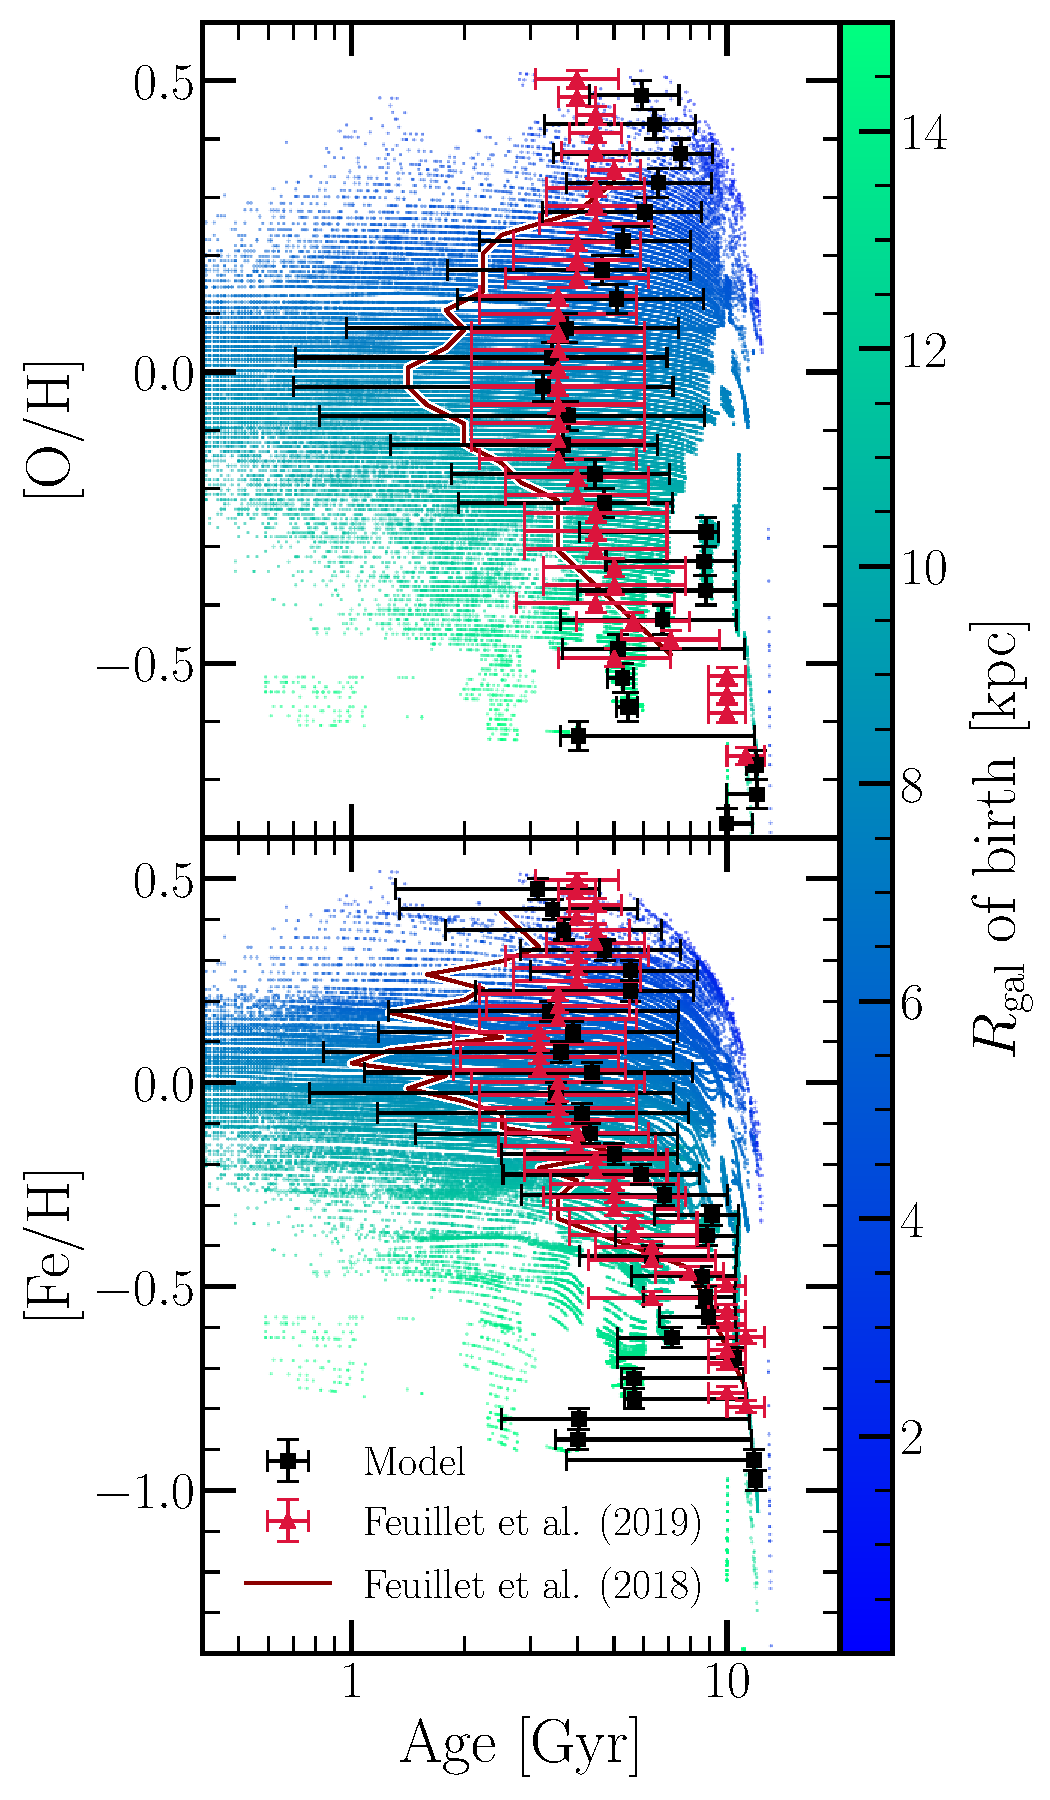
\includegraphics[scale = 0.45]{amr_solar_annulus.pdf} 
\caption{The age-[O/H] (top) and age-[Fe/H] (bottom) relations for the 
solar annulus (i.e.~$R_\text{gal}$ = 7 - 9 kpc,~$\left|z\right|\leq$ 0.5 kpc) 
as predicted by our inside-out SFH. Red triangles, black squares, error bars, 
and background points are as in Fig.~\ref{fig:age_alpha}, 
but with our simulation prediction quantified in 0.05-dex bins in [O/H] and 
[Fe/H]. For comparison, we plot the~\citet{Feuillet2018} data in a solid black 
line, omitting the associated uncertainties for the sake of clarity. } 
\label{fig:amr_solar_annulus} 
\end{figure} 

\begin{figure*} 
\centering 
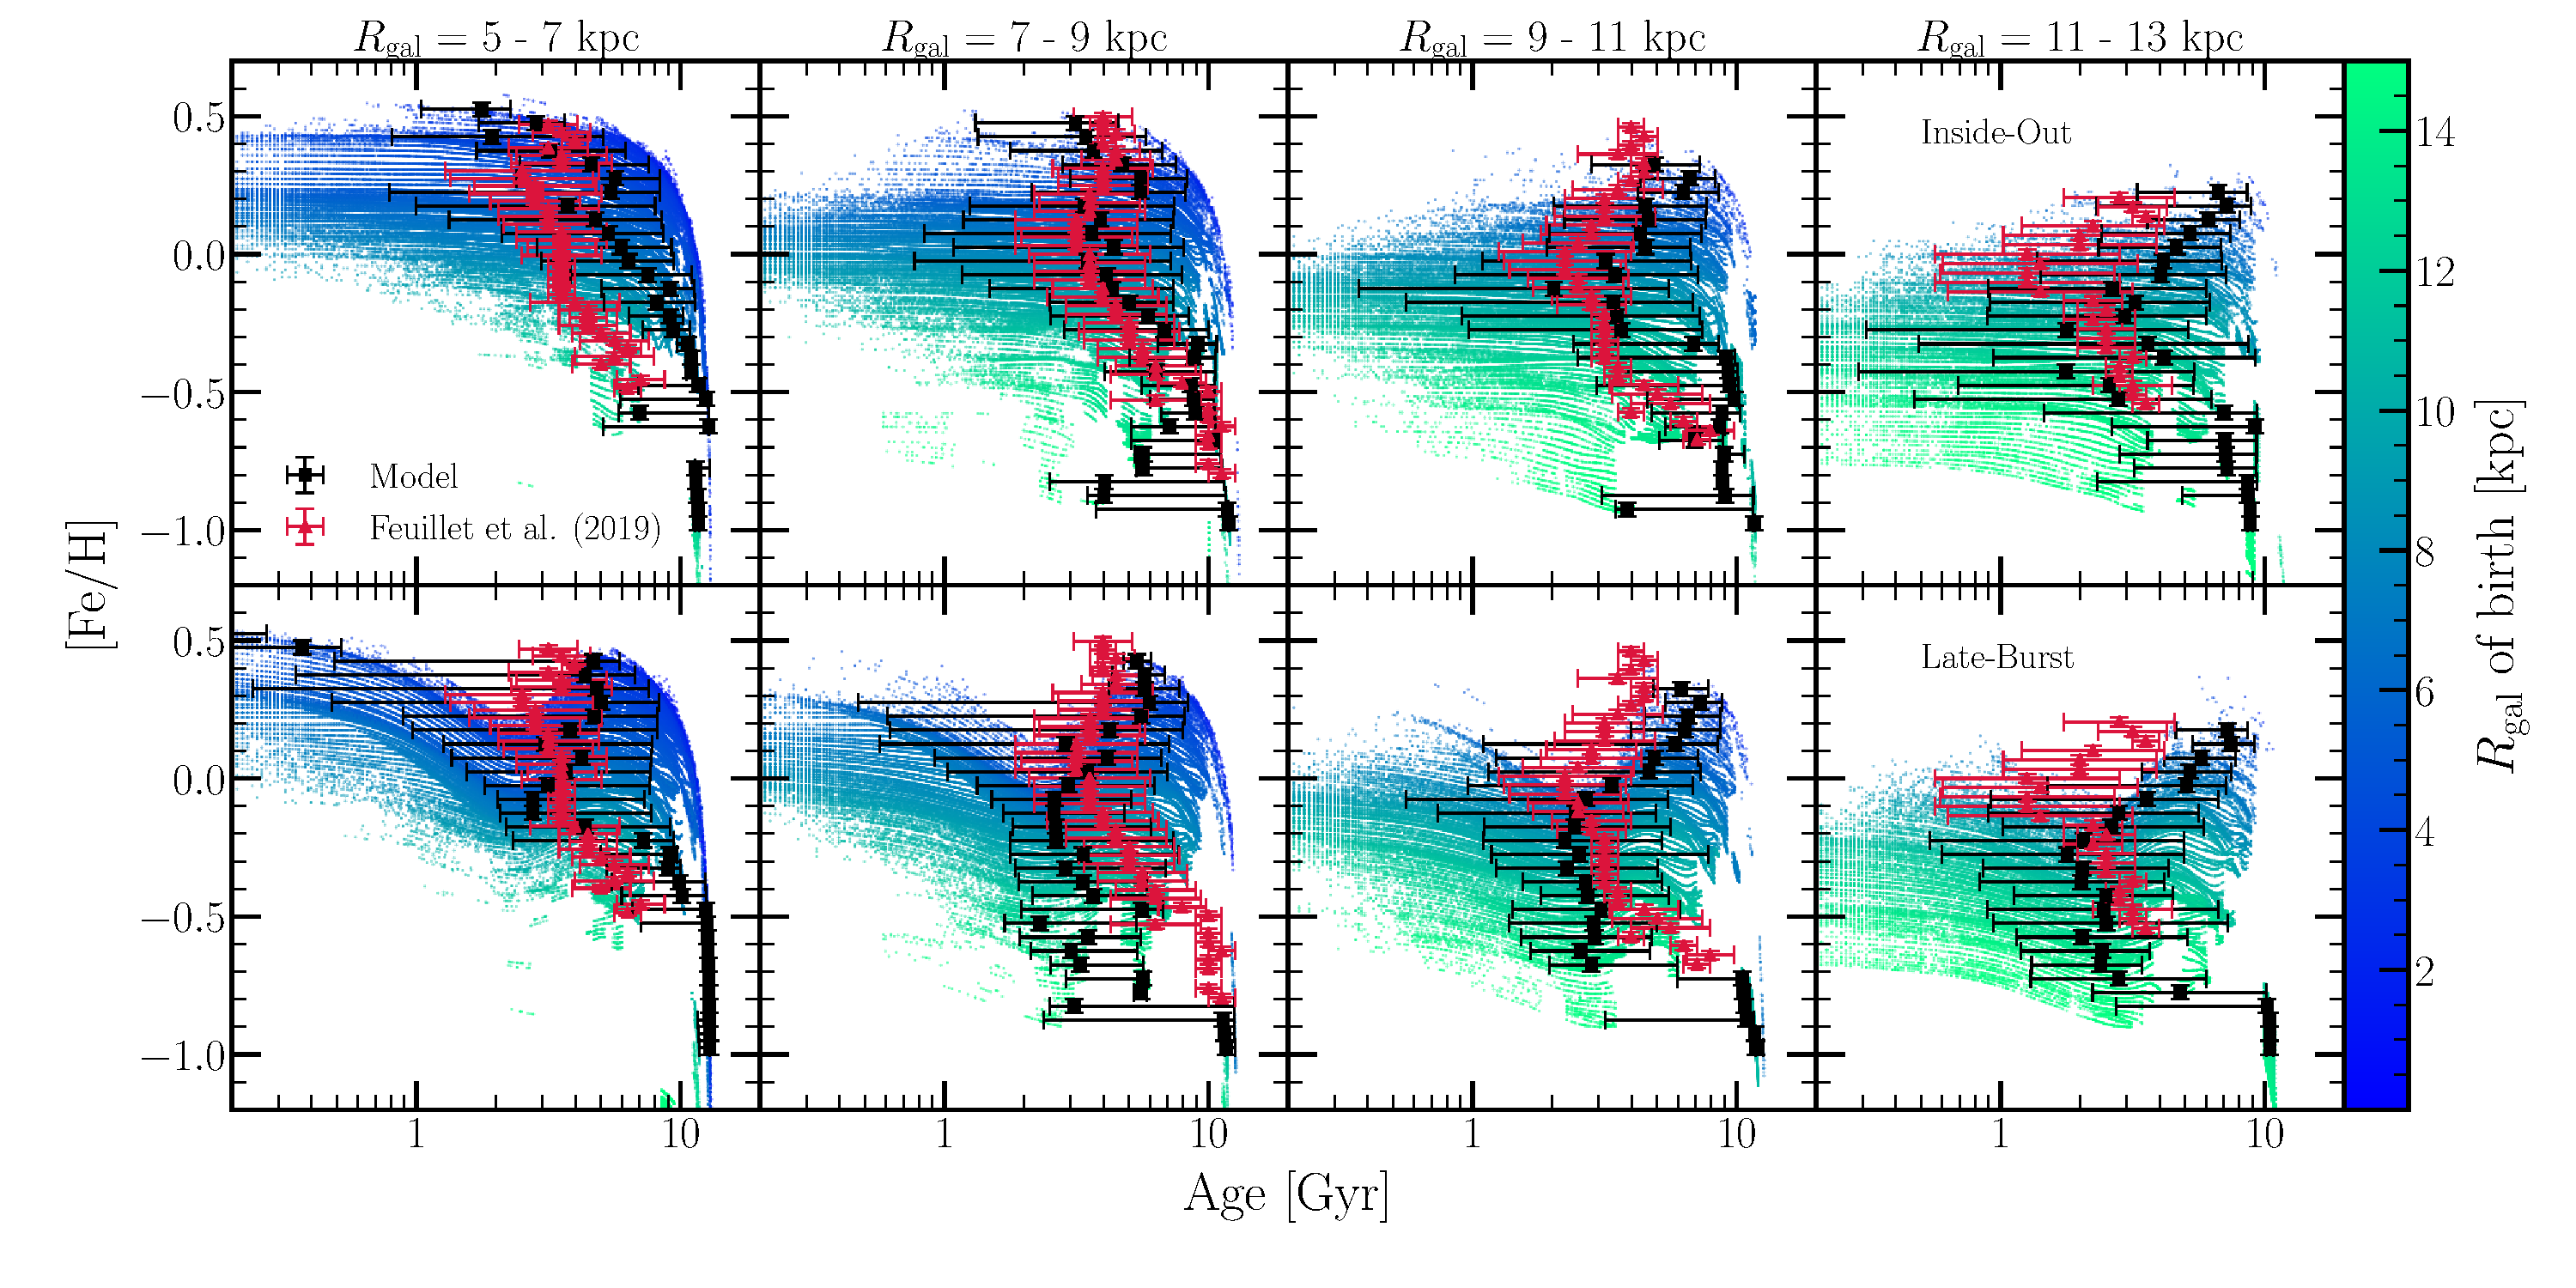
\includegraphics[scale = 0.35]{amr_insideout_vs_lateburst_fe.pdf} 
\caption{The age-[Fe/H] relation predicted by our inside-out (top) and 
late-burst (bottom) SFHs for~$R_\text{gal}$ = 5 - 7 kpc (left), 7 - 9 kpc 
(left middle), 9 - 11 kpc (right middle), and 11 - 13 kpc (right). Each panel 
plots only the~$\left|z\right|\leq$ 0.5 kpc population. Red triangles, black 
squares, error bars, and background points are as in 
Fig.~\ref{fig:age_alpha} for the corresponding 
Galactic region, but with our simulation prediction quantified in 
0.05-dex bins in [Fe/H]. } 
\label{fig:amr_insideout_vs_lateburst_fe} 
\end{figure*} 

% \begin{figure*} 
% \centering 
% \includegraphics[scale = 0.32]{amr_lateburst_Fe.pdf} 
% \caption{The age-[Fe/H] relation in 12 Galactic regions predicted by our 
% late-burst SFH. Bins in Galactocentric radius are shown in columns, and 
% labeled at the top. Bins in height~$\left|z\right|$ above/below the disc 
% midplane are shown in rows, noted in the left-hand column. Red triangles, 
% black squares, error bars, and background points are as in 
% Fig.~\ref{fig:age_alpha} for the corresponding Galactic 
% region, but with our simulated prediction quantified in 0.05-dex bins in 
% [Fe/H]. } 
% \label{fig:age_feh_regions} 
% \end{figure*} 

\begin{itemize} 
	\item Fig.~\ref{fig:age_oh_static} presents the age-[O/H] relation 
	predicted by our constant-SFH model for the~$\left|z\right|\leq$ 0.5 kpc 
	population at~$R_\text{gal}$ = 5 - 7, 7 - 9, 9 - 11, and 11 - 13 kpc. The 
	black points quantify the same mass-weighted median age in bins of 
	[O/H] as in~\S~\ref{sec:age_alpha}. Colored points in the background are 
	also the same - individual stellar populations color-coded according to 
	birth radius. 

	\item \citet{Feuillet2019} argued using the~\citet{Weinberg2017} analytic 
	models of chemical evolution that the non-monotonicity of the observed 
	AMR was due to radial migration. The youngest stars at a given radius 
	should reflect recent abundances of the local ISM, since young stars could 
	not have migrated significant distances. Old stars, however, could have 
	migrated from a wide range of radii, and can therefore reflect a wide 
	range of abundances. 

	\item Fig.~\ref{fig:age_oh_static} extends our understanding of this 
	effect. In all regions plotted, the intrinsic scatter in the bulk 
	age-[O/H] relation increases noticeably with increasing age, and the 
	color-coding of the background points makes it clear that this arises out 
	of radial migration. 

	\item Furthermore, the characteristic metallicity of the youngest stars 
	in a given radial bin decreases with increasing radius. This is a natural 
	consequence of the abundance gradient that we've built in at late times, 
	but interestingly, the effect is strong enough that at large radii, the 
	median trend is nearly monotonically increasing with age. This is 
	completely backwards from what is expected from one-zone models of 
	chemical evolution for any radius. Since this is our constant-SFR model, 
	it is not subject to the effects of a time-varying SFH, quantifying only 
	what is caused by radial migration. 

	\item Similar things are found for Fe, but the variations in the black 
	squares a bit bigger so we demonstrate the effect with [O/H]. 

	\item Fig.~\ref{fig:amr_solar_annulus} shows the age-[O/H] (top panel) 
	and the age-[Fe/H] (bottom panel) relations predicted by our fiducial 
	inside-out SFH in the solar annulus ($R_\text{gal}$ = 7 - 9 kpc and 
	$\left|z\right|\leq$~0.5 kpc), under the same plotting convention as in 
	\S~\ref{sec:age_alpha}. We add a solid black line to denote the 
	\citet{Feuillet2018} AMR in comparison to that of~\citet{Feuillet2019}. 
	\begin{itemize} 
		\item We note that we find similar results with regard to the 
		age-[O/H] relation predicted by our models. 

		\item \citet{Feuillet2018} shows a significantly younger median age at 
		solar metallicity in both O and Fe ($\sim$1 - 2 Gyr as opposed to 
		$\sim$2 - 3 Gyr). 

		\item Fiducial, inside-out SFH performs decently at explaining the 
		\citet{Feuillet2019} AMR, but the ages at solar metallicity in the 
		\citet{Feuillet2018} study are too young for this model. Comparing the 
		black points in this figure to those in Fig.~\ref{fig:age_oh_static} 
		suggests that the constant SFR model can't explain ages that young 
		either. If we were to take the~\citet{Feuillet2018} results at face 
		value in comparison to these models, this would strongly suggest a 
		recent enhancement at least in the local star formation rate of the 
		solar annulus to increase the frequency of~$\sim$1 Gyr old, solar 
		metallicity stars close to the sun. 

		\item Such a burst is indeed supported by the findings of 
		\citet{Mor2019}, who find a factor of~$\sim$2 enhancement in the SFH 
		of the Milky Way~$\sim$2 Gyr ago by comparing population synthesis 
		models to observed stellar luminosity functions and color-magnitude 
		diagrams with Gaia data~\citep{GaiaDR2}.~\citet{Isern2019} reach 
		similar conclusions modeling white dwarf luminosity functions in the 
		solar neighborhood with Gaia parallaxes. 
	\end{itemize} 

	\item Fig.~\ref{fig:amr_insideout_vs_lateburst_fe} shows a comparison of 
	the predicted age-[Fe/H] relation for~$\left|z\right|\leq$~0.5 kpc stars 
	in the~$R_\text{gal}$ = 5 - 7, 7 - 9, 9 - 11, and 11 - 13 kpc annuli. 
	Points are plotted in the same manner as in Fig.~\ref{fig:age_oh_static} 
	and Fig.~\ref{fig:amr_solar_annulus} in this section. 
	\begin{itemize} 
		\item Beyond the solar annuulus, we note that our inside-out SFH 
		model in general overpredicts the characteristic ages of stars 
		compared to~\citet{Feuillet2019} except for [Fe/H]~$\approx$~+0.4 and 
		-0.5. We also remark that in the trend is not very well reproduced 
		either, particularly in the~$R_\text{gal}$ = 5 - 7 kpc bin. 

		\item In the bottom row of panels, we show the same relation for our 
		late-burst SFH. Interestingly, the late-burst model improves upon the 
		failures of the inside-out model significantly. In particular, the 
		over-prediction of ages of solar and intermediate metallicity stars is 
		fixed by the late-burst model. 
		\begin{itemize} 
			\item In our recent starburst models,~\texttt{VICE} calculates 
			that there is a significant amount of zero metallicity gas infall 
			required to sustain such an increase in star formation under our 
			adopted~$\dot{\Sigma}_\star-\Sigma_\text{gas}$ relation (see 
			bottom two panels of Fig.~\ref{fig:evol} and~\S~
			\ref{sec:methods:sfe}). 

			\item Denoting the ages and compositions of the individual stellar 
			populations from our simulations, the colored points in the 
			background of these panels trace the metallicity of the gas as a 
			function of time at various radii. That is, the blue points also 
			represent the [Fe/H] of the gas phase at small radii at various 
			lookback times, and the same for the green points and large radii. 

			\item This demonstrates that at a lookback time of~$\sim$2 Gyr, by 
			construction, the ISM at nearly all Galactocentric radii decreased 
			in metallicity. At the same time, the star formation rates 
			increased by a factor of~$\sim$2, again by construction (see the 
			right-hand panels of Fig.~\ref{fig:evol}). The result is that at 
			any radius, the frequency of~$-0.5~\lesssim$~[O/H]~$\lesssim~0$ 
			stars at ages of~$\sim$2 Gyr is increases by a factor of~$\sim$2 
			from the inside-out model, decreasing the characteristic ages of 
			stars at these metallicities. 

			\item Although there appears to be an offset between the 
			\citet{Feuillet2019} data and our predicted AMR at high 
			$R_\text{gal}$, the late-burst model describes the observed trend 
			noticeably better than the inside-out model. Although the ages of 
			modestly sub-solar metallicity stars in the solar annulus are 
			slightly under-predicted by the model, the same can be said about 
			the trend here and at 5 - 7 kpc as well. 

			\item The parameters which control this offset are the yields of 
			Fe and the mass-loading factor as a function of~$R_\text{gal}$. 
			If we were to take a slightly higher yield of Fe, it would however 
			increase the overall normalization at~$R_\text{gal}$~< 9 kpc as 
			well, where we do not see this discrepancy. It's possible that the 
			mass-loading factor~$\eta$ (see discussion in~\S 
			\ref{sec:methods:yields}) increases too quickly at large 
			$R_\text{gal}$ in our models, or that outflows are more efficient 
			at removing individual elements from the star forming reservoir. 
			Variable metal-loading factors~$\eta_Z$ would be supported by the 
			observations of~\citet*{Chisholm2018}. 

			\item We remark that the late-burst model predicts extremely young 
			characteristic ages for the highest [Fe/H] bins in the 5 - 7 kpc 
			annulus. This is merely a consequence of the re-enrichment that 
			accompanies the ensuing starburst; in infall-driven starbursts 
			such as this, the abundances often reach super-equilibrium values 
			while the star formation rate is still perturbed, which then decay 
			together back to their pre-burst, equilibrium values 
			\citep{Johnson2020}. On 
			Fig.~\ref{fig:amr_insideout_vs_lateburst_fe}, this is noticeable 
			by the abundances on the left-hand edge of each panel being 
			higher in the late-burst scenario. The points that we have 
			plotted as characteristic ages represent that 50th percentile of 
			the mass-weighted age distribution of our stellar populations in 
			a bin of abundance; in other words, a mass-weighted 
			\textit{median}. The age-distribution at these abundances is 
			bimodal, noticeable by the colored points in the background, 
			indicating that the median may not be the best statistic for these 
			few stellar populations. We note that the outer-burst model, in 
			which $R_\text{gal}$~< 6kpc do not experience the starburst, does 
			not suffer from this issue. The minutia of the AMR at different 
			radii in our late starburst models is sensitive to the detailed 
			time-dependence of the straburst in each annulus. 
		\end{itemize} 
	\end{itemize} 

	\item Conclude that the AMR reported by~\citet{Feuillet2019} is better 
	described by our late starburst models than the inside-out model. This is 
	at odds with our findings in the same simulations with the same 
	observational dataset with regard to the age-[$\alpha$/Fe] relation. 
	Perhaps the differences can be reconciled. 
	\begin{itemize} 
		\item The models would be able to have their cake and eat it too if 
		there is a recent starburst with no ensuing $\alpha$-enhancement. This 
		is difficult to rationalize, however, because an increase in 
		[$\alpha$/Fe] in the wake of a starburst is a direct consequence of 
		the perturbed ratio of CCSN-SN Ia rates caused by the burst 
		\citep{Johnson2020}. We argue based on this that it is unlikely that 
		the detailed timing of a recent starburst would mitigate this issue. 

		\item It's possible that the Milky Way experienced dilution with no 
		ensuing starburst. This could be the case if the accreted gas was 
		mostly in the form of HI or HII that has not yet cooled and been 
		available for star formation, but has been mixing with the 
		nucleosynthetic products of ongoing star formation in the Galaxy. With 
		dilution playing a noticeable role in the AMR predicted by our burst 
		models, it's possible a model of this nature could agree with both 
		the AMR and the age-[$\alpha$/Fe] relation. This would require 
		future studies which include a treatment of a multi-phase ISM. 
	\end{itemize} 

	\item As a general result here, we caution future studies against 
	leveraging the agreement between a chemical evolution model and 
	observational data based on the solar annulus alone. Fig. 
	\ref{fig:amr_solar_annulus} presents the comparison of our fiducial, 
	inside-out SFH model predictions in the solar annulus to the 
	\citet{Feuillet2019} data, and Fig.~\ref{fig:amr_insideout_vs_lateburst_fe} 
	compares the inside-out and late-burst predictions in a larger range of 
	radii. Had we only considered the solar annulus, we would have concluded 
	that the fiducial, inside-out model agrees with the~\citet{Feuillet2019} 
	data well. However, in considering other regions of the Galaxy, we found 
	that the inside-out model actually had a handful of failures which were 
	mitigated by our late-burst model. 

	\item With our age-[O/H] and age-[Fe/H] relations, we find similar results 
	as in~\S~\ref{sec:age_alpha:beyond_solar_annulus} whereby our model 
	in general overpredicts the observed ages of stars at high 
	$\left|z\right|$. Discussion of potential sources of this can be found 
	in~\S~\ref{sec:age_alpha:beyond_solar_annulus}. 
\end{itemize} 

\section{Conclusions} 
\label{sec:conclusions} 
\begin{itemize} 
	\item We have modeled the Milky Way as a series of concentric annuli with 
	$\Delta R_\text{gal}$ = 100 pc width, describing each annulus as a 
	conventional one-zone model of chemical evolution, and allowing the 
	exchange of stellar populations between zones to model the impact of 
	stellar migration on enrichment in the Galaxy. The resulting ``multi-zone'' 
	is a technique that has received attention from only a handful of 
	chemical evolution studies to date~\citep{Matteucci1989, 
	Schoenrich2009, Minchev2013, Sharma2020}. In so doing, we adopted star 
	particles from the~\texttt{h277} zoom-in, hydrodynamical simulation to 
	describe the dynamical history of a Milky Way-like galaxy at face value. 
	This yields a model for radial migration which does not have any free 
	parameters (see discussion in~\S~\ref{sec:methods:h277}). 

	\item We found that similar numbers of star particles in~\texttt{h277} 
	migrated inward as outward, and that the two proceed on different 
	timescales, indicating that they're potentially linked to different 
	physical processes. We found that distributions of birth radii in bins of 
	final radii showing a mode which depends strongly on age is a 
	consequence of the surface density gradient. It's not that stars in general 
	migrate outward, it's simply that there are many many stars born at small 
	radii presently at large radii due to the fact that there are so many more 
	stars born at small radii, a consequence of the steep nature of the 
	surface density gradient~\citep[e.g.][]{Bland-Hawthorn2016}. 

	\item We found that the e-folding timescales for star formation indicated 
	by population averaged observations of Milky Way like galaxies are long 
	($\sim$15 Gyr in the solar annulus;~\citealp{Sanchez2020}). 

	\item We find that through stellar migration our models naturally 
	reproduce the observed result that high-$\alpha$ stars are more common at 
	small~$R_\text{gal}$ and high-$\left|z\right|$, and the opposite for 
	low-$\alpha$ stars (\citealp{Hayden2015}; see Fig. 
	\ref{fig:ofe_feh_diagram} and associated discussion in~\S 
	\ref{sec:metallicity_space}). 

	\item We demonstrate that the time-dependence of radial migration has a 
	significant impact on the [O/Fe] ratios as a function of time and radius 
	by inducing variability in the SN Ia rate and therefore the Fe abundance 
	(see Fig.~\ref{fig:tracks} and the associated discussion in~\S 
	\ref{sec:metallicity_space}). Although we haven't investigated it here, we 
	expect similar arguements to extend to other delayed sources such as AGB 
	stars and the associated s-process elements such as carbon, nitrogen, 
	strontium, yttrium, and zirconium. This is proof of concept that under 
	certain models for the time-dependence of radial migration, the migration 
	of nucleosynthetic yields proceeding alongside stellar migration is a 
	statistically significant effect. We therefore recommend future studies 
	relax the assumption that stars do not contribute to nucleosynthesis 
	beyond their birth radius. 

	\item We find that our models naturally reproduce the variations in the 
	observed metallicity distribution functions (MDFs) with Galactocentric 
	radius in the disc midplane ($\left|z\right|\leq$~0.5 kpc). At low 
	$R_\text{gal}$, the mode abundance in both [O/H] and [Fe/H] is high, and 
	conversely low at high~$R_\text{gal}$, with skewness in qualitative 
	agreement with the observations (\citealp[e.g.][]{Hayden2015}; see Fig. 
	\ref{fig:mdf_3panel_fe} and Fig.~\ref{fig:mdf_3panel_o} and the associated 
	discussion in~\S~\ref{sec:mdfs:oh_feh}). In some sense, 
	however, this is more a consequence of our building a realistic abundance 
	gradient into our models than a prediction on its own. In the observations, 
	the mode abundance in the midplane at $R_\text{gal}$ = 3 - 5 kpc is 
	strikingly similar to that at 5 - 7 kpc. Our models fail to reproduce this, 
	though it may be tied to a cessation of star formation in the inner 
	galaxy, as suggestted by~\citet{Peek2009} and~\citet{Fraternali2012}. Off 
	the midplane, our models predict a slight shift of the MDFs at small 
	$R_\text{gal}$ to lower metallicity, where in the observations, those for 
	all radii converge at [Fe/H]~$\approx$~[O/H]~$\approx$~-0.5. 

	\item We find that none of our models predict a Milky Way-like dichotomy 
	in [$\alpha$/Fe], as observed by many studies. The principle failure is 
	that the frequency of intermediate [$\alpha$/Fe] stars is overpredicted 
	relative to the observations (\citealp{Hayden2015}; Vincenzo et al. 2021, 
	in prep). This suggests that inside-out galaxy grouth combined with 
	radial migration, even if a recent starburst is included 
	\citep[e.g.][]{Mor2019, Isern2019}, is not adequate to explain the 
	observed dichotomy. This is at odds with the findings of 
	\citet{Sharma2020}, though we believe our study to have a more physically 
	motivated treatment of the chemical evolution models (see discussion in 
	\S~\ref{sec:mdfs:ofe}). The over-prediction of intermediate [$\alpha$/Fe] 
	stars in general suggests that shutting off star formation for the 
	intermediate-$\alpha$ phase would mitigate the problems suffered by our 
	models; we therefore postulate that a two-infall model may be necessary 
	to explain the observed dichotomy~\citep[e.g.][]{Chiappini1997, 
	Chiappini2001, Romano2010, Grisoni2017, Noguchi2018, Spitoni2016, 
	Spitoni2018, Spitoni2019, Spitoni2020}. Alternatively, we 
	speculate that the issues may be mitigated by an effective SN Ia yield of 
	Fe which depends inversely on metallicity, based on the findings of 
	\citet{Brown2019}. 

	\item We found that our recipe for setting the gradients in both stellar 
	surface density and metallicity yields the correct result. This is an 
	indication that radial migration does not change the profile of these 
	observed trends, only inducing scatter. 
	\begin{itemize} 
		\item We found that slightly different predictions in the stellar 
		and gas-phase metallicity gradient are natural consequences of 
		variations in the SFH. 

		\item We found that different models for the SFH predicted different 
		[O/Fe] gradients at the present day. 

		\item See Fig.~\ref{fig:metallicity_gradient} and the associated 
		disccusion in~\S~\ref{sec:metallicity_gradient} for the metallicity 
		gradient; Fig.~\ref{fig:surface_density} and discussion in 
		\S~\ref{sec:methods:surface_density_gradient} for the surface 
		density gradient. 
	\end{itemize} 

	\item We found that the observationally motivated approach to modeling the 
	efficiency of star formation ($\tau_\star \equiv \Sigma_\text{gas} / 
	\dot{\Sigma}_\star$) adopted in our simulations in general overpredicts 
	the molecular fractions by mass of the model Galaxy. The discrepancy arose 
	out of an underabundance of HI/HII rather than an overabundance of H$_2$ 
	in the global demographics predicted by our simulation. Nonetheless, we 
	demonstrate in Appendix~\ref{sec:sfe_variations} that relaxing these 
	assumptions do not impact our model predictions. We also discuss a handful 
	of potential sources of the discrepancy there. 

	\item We found that the time-dependence of radial migration indeed does 
	have an impact on enrichment. Previous studies in the literature have 
	assumed that this is not the case, due to the slow nature of migration 
	\citep[e.g.][]{Minchev2013}. However, we find that even for young stars, 
	the tails of the present-day $R_\text{gal}$ distribution are adequately 
	long that when age-dependent migration is taken into account, the model 
	predicts variations in the SN Ia rate that then impact predicted abundance 
	ratios. We demonstrated that this is a means with which stellar migration 
	may produce young, Fe-poor stars which can migrate to the solar annulus, 
	and potentially be misinterpreted as young, $\alpha$-rich stars. This is 
	proof of concept that the radial migration of nucleosynthetic yields can 
	proceed alongside the radial migration of stars, depending on which model 
	for migration that you believe. 
	\begin{itemize} 
		\item These stars have been seen in observed data from APOGEE 
		\citep[e.g.][]{SilvaAguirre2018}. They postulate that since these stars 
		have kinematics similar to the rest of the high-$\alpha$ population, 
		that perhaps they are the consequence of stellar mergers or mass 
		transfer events, producing truly old stars that simply appear to be 
		younger. While these interpretations are not mutually exclusive, an 
		observational test to ascertain the origins of the observed young 
		$\alpha$-rich population would have implications for which of the 
		models for radial migration investigated here are the most realistic. 
	\end{itemize} 

	\item In the observations, the high-$\alpha$ sequence is known to be most 
	prominent at low~$R_\text{gal}$ and high~$\left|z\right|$, and conversely, 
	the low-$\alpha$ population at high~$R_\text{gal}$ and low~$\left|z\right|$ 
	\citep[e.g.][]{Hayden2015}.  We found that this is a natural consequence of 
	stellar migration, though the detailed distributions depend on the SFH and 
	the relative yields of $\alpha$ and iron-peak elements, both of which are 
	highly uncertain, and we do not model them in detail here. 

	\item We found that our inside-out model predicts an age-[$\alpha$/Fe] 
	relation which is in good agreement with the observed relation reported 
	by~\citet{Feuillet2019}. Our recent starburst models predict a global 
	$\alpha$-enhancement that simply isn't seen in the data. This suggests 
	that our current understanding of chemical evolution may be at odds with 
	the findings of~\citet{Mor2019} and~\citet{Isern2019} suggesting a recent 
	factor of~$\sim$2 enhancement in the Milky Way SFH peaking~$\sim$2 Gyr ago. 

	\item We find that where our recent starburst models fail to agree with 
	the age-[O/Fe] relation reported by~\citet{Feuillet2019}, it tends to 
	overpredict ages at a given [O/Fe]. However, it tends to fail in a manner 
	such that the~\citet{Feuillet2019} relation agrees with the stars that we 
	would call Fe-poor - that is, the stars that are $\alpha$-enhanced due to 
	forming out of an Fe-poor ISM due to the same variations in the SN Ia rate 
	that can produce young, $\alpha$-rich stars. While this may be coincidence, 
	if we take the observations at face value, it would suggest that our model 
	is overpredicting the rate of Fe injection, and that perhaps SN Ia yields 
	of Fe should be lower. If we take the model at face value, it suggests that 
	APOGEE+Gaia targets preferentially sample young, $\alpha$-rich stars 
	(\citealp{Feuillet2019} used APOGEE data for stars with Gaia parallaxes). 

	\item We found that the age-metallicity relation (AMR) in both [O/H] and 
	[Fe/H] reported by~\citet{Feuillet2019} is better fit by our late 
	starburst models. This is at odds with the findings regarding the 
	age-[O/Fe] relation, where the inside-out model agreed with the data much 
	better than the starburst models. This is interesting, because different 
	observables are favoring different models for the SFH, suggesting that 
	something more complicated is going on. 
	\begin{itemize} 
		\item The starburst models agreeing with the observed AMR has to do 
		with dilution as well as the starburst itself. It's possible that the 
		Milky Way experienced a dilution event that was primarily HI/HII gas 
		that has not yet cooled to be available for star formation. This could 
		mitigate the discrepancy. It would, however, be at odds with the 
		observed results of~\citet{Mor2019} and~\citet{Isern2019} suggesting 
		such a recent enhancement in star formation. 

		\item Off the midplane, our model-predicted AMR overestimates ages 
		relative to~\citet{Feuillet2019}, just like in the age-[O/Fe] relation. 
		We speculate that this may be related to the Sagitarrius dwarf 
		galaxy; it's important to remember that our model galaxy does not have 
		the Milky Way's dynamical history, but~\texttt{h277}'s dynamical 
		history. {\color{red} Jon and I are looking into this, but as I 
		understand it, what I've written next is in general true.}~\texttt{h277} 
		did not have a Sagitarrius-like accretion event. Since Sagitarrius 
		has made multiple pericentric passages nearly head-on with the Milky 
		Way disc, it's possible that young stars were kinematically heated to 
		high~$\left|z\right|$, an effect that would not be present in 
		\texttt{h277} without such an event. This would decrease our model 
		predicted median ages at these heights by directly adding more young 
		stars, and potentially not having noticeable effect in the midplane due 
		to the much larger number of stars there. 
	\end{itemize} 

	\item We remark on the low number of multi-zone 
	chemical evolution models in the literature. We call for more studies 
	which adopt a similar approach; with only a handful of simulations which 
	can be ran in a combined time interval of less than a single working day, 
	we were able to assess model predictions of various chemical evolution 
	scenarios in comparison to a wide range of observables. With a wealth of 
	one-zone chemical evolution models (both numerical and analytic) and 
	high-resolution hydrodynamical simulations already in the literature, 
	there is a true void in the literature for these medium resolution, medium 
	computational expense models which which can teach us a great deal about 
	the enrichment history of the Milky Way. For this reason,~\texttt{VICE} 
	is open source software, and its~\texttt{milkyway} object which ran our 
	simulations adopts many of this paper's physically and observationally 
	motivated assumptions as default values. Alternative zone configurations 
	can be achieved by subclassing the~\texttt{multizone} object and 
	specifying how gas and stars should move between the individual zones, as 
	we have already done for the~\texttt{milkyway} object. 

	\item \texttt{VICE} is publicly available and open-source. It can be 
	installed via~\texttt{pip} (\url{https://pypi.org/project/vice}). 
	Documentation is available at~\url{https://vice-astro.readthedocs.io}. 
	Source code is hosted at~\url{https://github.com/giganano/VICE.git}. 
	\texttt{Python} code which runs the simulations presented in this paper 
	are included as supplementary material in the~\texttt{git} repository; 
	our models can be ran directly from a~\texttt{bash} terminal without 
	modifying the source code, and are capable of predicting abundances for 
	$\sim$2 million stellar populations in only~$\sim$2 CPU hours with a 
	single core on personal computers. 
\end{itemize} 

\section{Acknowledgements} 
\label{sec:acknowledgements} 
We are grateful to Diane Feuillet for sharing the data 
from~\citet{Feuillet2018} and~\citet{Feuillet2019} with us. {\color{red} There 
will be others added, depending on whether or not they go here or on the 
author's list. I'll also need to add the SDSS acknowledgements since we made 
use of APOGEE data.} 
\par 
\textit{Software}: Matplotlib~\citep{Matplotlib}; Astropy~\citep{Astropy2013, 
Astropy2018}; NumPy~\citep{NumPy}. 

\section{Data Availability} 
{\color{red} In case anyone hasn't seen one of these Data Availability 
statements yet, this is now a requirement by MNRAS. It wasn't when I submitted 
my last paper, but was by the time we were finished with the referee report, 
so I wound up having to add one. They just want you to say if the data are 
available to the reader or not, and where/how they can get it if they are. }
\texttt{VICE} is open source software, and as such the source code for these 
simulations is publicly available.\footnote{
	\url{https://pypi.org/project/vice} \\ 
	\url{https://vice-astro.readthedocs.io} \\ 
	\url{https://github.com/giganano/VICE.git} 
} The source code which produces the outputs presented in this paper as well as 
the figures are included as secondary material in the GitHub repository. 
While the aggregate of all outputs analyzed in this paper are sufficiently 
large that it is not conducive to store them on GitHub, we provide instructions 
on how to run our simulations and variations thereof. All observational data 
appearing in this paper is publicly available, and is also included with the 
source code for our simulations and figures. 

\newpage 
\begin{appendices} 

\section{Normalizing a Fiducial Star Formation History} 
\label{sec:normalize_sfh} 
\begin{itemize} 
	\item Derive formula for normalizing an SFH given the time-dependence at 
	a given radius $f(t|R_\text{gal})$ and the radial dependence of the 
	desired surface density gradient at late times $g(R_\text{gal})$. Neither 
	need be normalized. 
	\begin{equation} 
	\dot{\Sigma}_\star(R_\text{gal}, t) = \dot{\Sigma}_{\star,0}(R_\text{gal}) 
	f(t|R_\text{gal}) 
	\end{equation} 
	\begin{equation} 
	\Sigma_\star(r) = \Sigma_{\star,0} g(R_\text{gal}) 
	\end{equation} 

	\item Integrate surface density of star formation with time and you get 
	the present day surface density gradient at that radius. This yields the 
	unknown $\dot{\Sigma}_{\star,0}$ in terms of $\Sigma_\star(R_\text{gal})$ 
	and subsequently the unknown $\Sigma_{\star,0}$. 
	\begin{subequations}\begin{align} 
	\Sigma_\star(R_\text{gal}) 
	&\approx (1 - r) \int_0^T \dot{\Sigma}_\star(R_\text{gal}, t) dt \\ 
	&= (1 - r) \dot{\Sigma}_{\star,0}(R_\text{gal}) \int_0^T f(t|R_\text{gal}) 
	dt \\ 
	\implies \dot{\Sigma}_{\star,0}(R_\text{gal}) &= 
	\Sigma_\star(R_\text{gal}) \left[(1 - r)\int_0^T f(t|R_\text{gal}) dt
	\right]^{-1} \\ 
	&= \Sigma_{\star,0}g(R_\text{gal}) \left[(1 - r) \int_0^T f(t|R_\text{gal}) 
	dt\right]^{-1} 
	\end{align}\end{subequations} 

	\item Integrate surface density over area of the disc and you get the 
	present day Milky Way stellar mass. This solves for the unknown 
	$\Sigma_{\star,0}$: 
	\begin{subequations}\begin{align} 
	M_\star^\text{MW} &= \int_0^R \Sigma_\star(R_\text{gal}) 2\pi R_\text{gal} 
	dR_\text{gal} \\ 
	&= \Sigma_{\star,0}\int_0^R g(R_\text{gal}) 2\pi R_\text{gal} dR_\text{gal} 
	\\ 
	\implies \Sigma_{\star,0} &= M_\star^\text{MW} 
	\left[\int_0^R g(R_\text{gal}) 2\pi R_\text{gal}dR_\text{gal}\right]^{-1} 
	\end{align}\end{subequations} 

	\item Combine the last two equations into 
	$\dot{\Sigma}_\star(R_\text{gal}, t)$ and obtain the following equation: 
	\begin{equation} 
	\dot{\Sigma}_\star(R_\text{gal}, t) = A f(t|R_\text{gal}) g(R_\text{gal}) 
	\end{equation} 
	where 
	\begin{equation} 
	A = M_\star^\text{MW}\left[(1 - r)\int_0^R g(R_\text{gal}) 2\pi 
		R_\text{gal} dR_\text{gal} \int_0^T f(t|R_\text{gal}) dt\right]^{-1} 
	\end{equation} 
	This result makes intuitive sense: $f(t|R_\text{gal})$ specifies the 
	time-dependence of the SFH and $g(R_\text{gal})$ specifies the radial 
	dependence by construction, and $M_\star^\text{MW}$ sets the overall 
	normalization. 

	\item This recipe implicitly assumes that radial migration does not 
	significantly alter the surface density profile, and we have demonstrated 
	in~\S~\ref{sec:methods:surface_density_gradient} that this is the case for 
	the Galactocentric radii of interest in this paper. It introduces scatter, 
	but does not alter the overall dependence. This recipe can be employed in 
	disc galaxy models as long as this is not violated. 
\end{itemize} 

\newpage 
\section{Variations in Star Formation Efficiency} 
\label{sec:sfe_variations} 
{\color{red} It'd be good to present a comparison of our fiducial, inside-out 
SFH model to a case where we make a significantly different assumption about 
$\tau_\star$, and demonstrate that it doesn't impact the conclusions. This 
could motivate some of the discussion below as well, so that this Appendix can 
still tell a generally interesting story beyond just a comparison. }

\begin{itemize} 
	\item {\color{red} Here are some of my thoughts on what could be 
	causing the discrepancy with this $\tau_\star$ business. Since 
	this is for discussion purposes, I haven't looked in detail at any 
	of this; I'm simply speculating for the sake of discussion in the 
	text. } 

	\item As discussed in~\S~\ref{sec:methods:sfe}, our fiducial inside-out 
	SFH overpredicts the molecular fraction~$f_\text{mol}$ relative to 
	observed results in the Milky Way. This is a result of both an 
	underpredicted HI + HII mass and an overpredicted H$_2$ mass. The 
	predicted HI + HII mass is~$5.54\times10^9$~M$_\odot$ relative to an 
	observed value of~$\sim10^{10}$~M$_\odot$~\citep{Kalberla2009}. The 
	predicted H$_2$ mass is~$7.14\times10^9$~M$_\odot$, compared to an 
	observed values of~$2.5\times10^9$~M$_\odot$ from~\citet{Kalberla2009} and 
	$1\times10^9$~M$_\odot$ from~\citet{Heyer2015}. Here we discuss potential 
	sources of this discrepancy, and demonstrate that the assumed form of the 
	star formation law does not impact our conclusions. 

	\item First, the overpredicted H$_2$ mass. Our fiducial inside-out model, 
	whose SFH is normalized to predict the same total stellar mass as that 
	reported by~\citet{Licquia2015} with the surface density gradient of 
	\citet{Bland-Hawthorn2016} (see discussion in~\S~\ref{sec:methods:sfhs} 
	and~\ref{sec:methods:surface_density_gradient}). This model predicts a 
	present-day SFR of 4.89 M$_\odot$~yr$^{-1}$, an overprediction relative to 
	the observed value of 1.65 M$_\odot$~yr$^{-1}$~\citep{Licquia2015}. 
	However, our model predicts a gradient in the present-day surface density 
	of star formation with radius which decreases monotonically (see the top 
	row, left-center panel of Fig.~\ref{fig:evol}), whereas the observations 
	of \citet{Peek2009} and~\citet{Fraternali2012} would suggest that the 
	Milky Way has begun the process of inside-out quenching. Fig. 2 of 
	\citet{Fraternali2012} suggests that the surface density of star 
	formation is significantly lower within~$R_\text{gal} \lesssim$ 4 kpc. 
	Cutting off our summation of the H$_2$ mass and present-day SFR at 
	4 kpc yields a present-day star formation rate of 3.06 M$_\odot$ 
	yr$^{-1}$, and an H$_2$ mass of~$4.48\times10^9$~M$_\odot$, still an 
	overprediction relative to~\citet{Licquia2015} and 
	\citet{Kalberla2009}. Instead cutting the summation off at 6 kpc 
	yields $\dot{M}_\star$ = 1.97 M$_\odot$~yr$^{-1}$ and H$_2$ = 
	$2.88\times10^9$~M$_\odot$, still a slight overprediction, but in 
	better agreement still. Based on these calculations, we argue that the 
	overpredicted H$_2$ mass in our fiducial inside-out model is a consequence 
	of an overpredicted SFR at the present day. A model with either a more 
	steeply declining SFH or quenching of star formation in the inner Galaxy 
	as suggested by~\citet{Peek2009} and~\citet{Fraternali2012} should resolve 
	this discrepancy. 

	\item Next, the under-predicted HI + HII mass. We speculate over a couple 
	possible explanations of this. 
	\begin{itemize} 
		\item At first glance, this could point to a breakdown in the 
		fundamental assumption of our adopted model for star formation 
		efficiency. As discussed in~\S~\ref{sec:methods:sfe}, we adopte the 
		assumption that our model Galaxy follows the observed trend in the 
		mean~$\dot{\Sigma}_\star-\Sigma_\text{gas}$ relation, even though 
		there is evidence that individual galaxies do not follow such a 
		relation~\citep{Ellison2020b}.~\citet{Kennicutt2020} however argue 
		that such a prescription should still be a valid recipe in galaxy 
		evolution models. 

		\item An important caveat in understanding our ISM masses is that 
		because we treat the ISM as being available for star formation in its 
		entirety, they therefore track only the amount of gas in the 
		\textit{star forming reservoir}. Zero metallicity gas infall simply 
		appears in each annulus to balance the amount of gas lost to star 
		formation and outflows at each timestep in order to sustain the 
		level of star formation at the next timestep. Based on our model, if 
		gas is removed from the star forming reservoir, but remains in a 
		spatially confined region reasonably defining the Galaxy, our model 
		will treat it it as an outflow and remove it from the ISM, though in 
		nature it would still show up in observations and be counted as part 
		of the Milky Way's gas content. {\color{red} It's therefore plausible 
		that the difference could simply be nuanced semantics regarding what 
		we refer to as an outflow numerically and what would be considered an 
		outflow in an observational study (i.e. ejection from the disc).} 
		\begin{itemize} 
			\item Based on this argument, one potential source of the 
			difference could be infall from the circum- and inter-galactic 
			media that have not yet been made available for star formation. 
			This would show up as HI and HII observed in the ISM, but would 
			not be counted in our models if it is not yet incorporated into 
			the star forming reservoir. 

			\item Another potential source could be star formation efficiency 
			in the meaning that the ISM/feedback literature often takes: the 
			fraction of molecular cloud masses that are converted into stars. 
			To first order, this value is a few percent with some intrinsic 
			scatter ({\color{red} citation}). This means that in our models, 
			a significant multiplier ($\sim$30) of the stellar mass formed in 
			a given timestep should be added to the hot phase of the ISM in 
			the form of HII through feedback processes. If this gas is never 
			again made available for star formation, our model would treat it 
			as an outflow, removing it from the ISM mass, while in nature it 
			is still observed within the reasonably confined region defining 
			the Galaxy. 

			\item Together, these effects may constitute the remaining factor 
			of~$\sim$ of warm and hot gas that our fiducial model is missing. 
			However, an investigation of the impact of a multi-phase ISM on 
			models such as these is outside the scope of this paper. 
		\end{itemize} 
	\end{itemize} 

	\item Whatever the source of this discrepancy may be, the decision 
	about the mathematical form of~$\tau_\star$ does not significantly 
	impact our conclusions, as demonstrated in the remainder of this Appendix. 
\end{itemize} 

\end{appendices} 

\newpage 
\bibliographystyle{mnras} 
\bibliography{outline2} 

\label{lastpage} 
\end{document} 

